% Options for packages loaded elsewhere
\PassOptionsToPackage{unicode}{hyperref}
\PassOptionsToPackage{hyphens}{url}
%
\documentclass[
]{book}
\usepackage{amsmath,amssymb}
\usepackage{iftex}
\ifPDFTeX
  \usepackage[T1]{fontenc}
  \usepackage[utf8]{inputenc}
  \usepackage{textcomp} % provide euro and other symbols
\else % if luatex or xetex
  \usepackage{unicode-math} % this also loads fontspec
  \defaultfontfeatures{Scale=MatchLowercase}
  \defaultfontfeatures[\rmfamily]{Ligatures=TeX,Scale=1}
\fi
\usepackage{lmodern}
\ifPDFTeX\else
  % xetex/luatex font selection
\fi
% Use upquote if available, for straight quotes in verbatim environments
\IfFileExists{upquote.sty}{\usepackage{upquote}}{}
\IfFileExists{microtype.sty}{% use microtype if available
  \usepackage[]{microtype}
  \UseMicrotypeSet[protrusion]{basicmath} % disable protrusion for tt fonts
}{}
\makeatletter
\@ifundefined{KOMAClassName}{% if non-KOMA class
  \IfFileExists{parskip.sty}{%
    \usepackage{parskip}
  }{% else
    \setlength{\parindent}{0pt}
    \setlength{\parskip}{6pt plus 2pt minus 1pt}}
}{% if KOMA class
  \KOMAoptions{parskip=half}}
\makeatother
\usepackage{xcolor}
\usepackage{color}
\usepackage{fancyvrb}
\newcommand{\VerbBar}{|}
\newcommand{\VERB}{\Verb[commandchars=\\\{\}]}
\DefineVerbatimEnvironment{Highlighting}{Verbatim}{commandchars=\\\{\}}
% Add ',fontsize=\small' for more characters per line
\usepackage{framed}
\definecolor{shadecolor}{RGB}{248,248,248}
\newenvironment{Shaded}{\begin{snugshade}}{\end{snugshade}}
\newcommand{\AlertTok}[1]{\textcolor[rgb]{0.94,0.16,0.16}{#1}}
\newcommand{\AnnotationTok}[1]{\textcolor[rgb]{0.56,0.35,0.01}{\textbf{\textit{#1}}}}
\newcommand{\AttributeTok}[1]{\textcolor[rgb]{0.13,0.29,0.53}{#1}}
\newcommand{\BaseNTok}[1]{\textcolor[rgb]{0.00,0.00,0.81}{#1}}
\newcommand{\BuiltInTok}[1]{#1}
\newcommand{\CharTok}[1]{\textcolor[rgb]{0.31,0.60,0.02}{#1}}
\newcommand{\CommentTok}[1]{\textcolor[rgb]{0.56,0.35,0.01}{\textit{#1}}}
\newcommand{\CommentVarTok}[1]{\textcolor[rgb]{0.56,0.35,0.01}{\textbf{\textit{#1}}}}
\newcommand{\ConstantTok}[1]{\textcolor[rgb]{0.56,0.35,0.01}{#1}}
\newcommand{\ControlFlowTok}[1]{\textcolor[rgb]{0.13,0.29,0.53}{\textbf{#1}}}
\newcommand{\DataTypeTok}[1]{\textcolor[rgb]{0.13,0.29,0.53}{#1}}
\newcommand{\DecValTok}[1]{\textcolor[rgb]{0.00,0.00,0.81}{#1}}
\newcommand{\DocumentationTok}[1]{\textcolor[rgb]{0.56,0.35,0.01}{\textbf{\textit{#1}}}}
\newcommand{\ErrorTok}[1]{\textcolor[rgb]{0.64,0.00,0.00}{\textbf{#1}}}
\newcommand{\ExtensionTok}[1]{#1}
\newcommand{\FloatTok}[1]{\textcolor[rgb]{0.00,0.00,0.81}{#1}}
\newcommand{\FunctionTok}[1]{\textcolor[rgb]{0.13,0.29,0.53}{\textbf{#1}}}
\newcommand{\ImportTok}[1]{#1}
\newcommand{\InformationTok}[1]{\textcolor[rgb]{0.56,0.35,0.01}{\textbf{\textit{#1}}}}
\newcommand{\KeywordTok}[1]{\textcolor[rgb]{0.13,0.29,0.53}{\textbf{#1}}}
\newcommand{\NormalTok}[1]{#1}
\newcommand{\OperatorTok}[1]{\textcolor[rgb]{0.81,0.36,0.00}{\textbf{#1}}}
\newcommand{\OtherTok}[1]{\textcolor[rgb]{0.56,0.35,0.01}{#1}}
\newcommand{\PreprocessorTok}[1]{\textcolor[rgb]{0.56,0.35,0.01}{\textit{#1}}}
\newcommand{\RegionMarkerTok}[1]{#1}
\newcommand{\SpecialCharTok}[1]{\textcolor[rgb]{0.81,0.36,0.00}{\textbf{#1}}}
\newcommand{\SpecialStringTok}[1]{\textcolor[rgb]{0.31,0.60,0.02}{#1}}
\newcommand{\StringTok}[1]{\textcolor[rgb]{0.31,0.60,0.02}{#1}}
\newcommand{\VariableTok}[1]{\textcolor[rgb]{0.00,0.00,0.00}{#1}}
\newcommand{\VerbatimStringTok}[1]{\textcolor[rgb]{0.31,0.60,0.02}{#1}}
\newcommand{\WarningTok}[1]{\textcolor[rgb]{0.56,0.35,0.01}{\textbf{\textit{#1}}}}
\usepackage{longtable,booktabs,array}
\usepackage{calc} % for calculating minipage widths
% Correct order of tables after \paragraph or \subparagraph
\usepackage{etoolbox}
\makeatletter
\patchcmd\longtable{\par}{\if@noskipsec\mbox{}\fi\par}{}{}
\makeatother
% Allow footnotes in longtable head/foot
\IfFileExists{footnotehyper.sty}{\usepackage{footnotehyper}}{\usepackage{footnote}}
\makesavenoteenv{longtable}
\usepackage{graphicx}
\makeatletter
\def\maxwidth{\ifdim\Gin@nat@width>\linewidth\linewidth\else\Gin@nat@width\fi}
\def\maxheight{\ifdim\Gin@nat@height>\textheight\textheight\else\Gin@nat@height\fi}
\makeatother
% Scale images if necessary, so that they will not overflow the page
% margins by default, and it is still possible to overwrite the defaults
% using explicit options in \includegraphics[width, height, ...]{}
\setkeys{Gin}{width=\maxwidth,height=\maxheight,keepaspectratio}
% Set default figure placement to htbp
\makeatletter
\def\fps@figure{htbp}
\makeatother
\setlength{\emergencystretch}{3em} % prevent overfull lines
\providecommand{\tightlist}{%
  \setlength{\itemsep}{0pt}\setlength{\parskip}{0pt}}
\setcounter{secnumdepth}{5}
\usepackage{booktabs}
\ifLuaTeX
  \usepackage{selnolig}  % disable illegal ligatures
\fi
\usepackage[]{natbib}
\bibliographystyle{plainnat}
\IfFileExists{bookmark.sty}{\usepackage{bookmark}}{\usepackage{hyperref}}
\IfFileExists{xurl.sty}{\usepackage{xurl}}{} % add URL line breaks if available
\urlstyle{same}
\hypersetup{
  pdftitle={R Workshop},
  pdfauthor={Dilan Caro},
  hidelinks,
  pdfcreator={LaTeX via pandoc}}

\title{R Workshop}
\author{Dilan Caro}
\date{2024-06-12}

\begin{document}
\maketitle

{
\setcounter{tocdepth}{1}
\tableofcontents
}
\chapter*{Welcome}\label{welcome}
\addcontentsline{toc}{chapter}{Welcome}


\includegraphics[width=1\linewidth]{images/CU STAR}

Are you ready to embark on an exciting journey into the world of data analysis and statistical exploration? Imagine having the power to unlock the hidden insights within vast datasets, create stunning visualizations, and make data-driven decisions that can shape the future. Welcome to the world of R programming! R is not just a language; it's your key to uncovering the stories data has to tell. Whether you're a budding data scientist, a curious researcher, or someone who simply loves solving puzzles, R offers you a thrilling adventure where you'll learn to command data with precision and creativity. Get ready to be amazed by the endless possibilities of R and join a global community of data enthusiasts who are reshaping the world, one analysis at a time.

In this website, you will have resources, examples and practice to master R.\footnote{Disclaimer: The logos and names of Columbia University are used with permission for the purpose of this workshop only. The content and opinions expressed in these materials are solely those of the author and do not represent the views or policies of Columbia University. Columbia University is not responsible for any content or representations made within these materials.}

Our Github repository will contain materials, cheat sheets and more. Find it \href{https://github.com/DilanCaro/CU-R-Workshop}{here} or below.

\url{https://github.com/DilanCaro/CU-R-Workshop}

\section*{Objectives}\label{objectives}
\addcontentsline{toc}{section}{Objectives}

\section*{Session 1: R Basics (1 hour 45 min)}\label{session-1-r-basics-1-hour-45-min}
\addcontentsline{toc}{section}{Session 1: R Basics (1 hour 45 min)}

\subsection*{Part 1: Introduction to R}\label{part-1-introduction-to-r}
\addcontentsline{toc}{subsection}{Part 1: Introduction to R}

\begin{enumerate}
\def\labelenumi{\arabic{enumi}.}
\tightlist
\item
  What is R and why use it?
\item
  Installing R and RStudio
\item
  Basic RStudio layout and functionality
\end{enumerate}

\subsection*{Part 2: R Fundamentals}\label{part-2-r-fundamentals}
\addcontentsline{toc}{subsection}{Part 2: R Fundamentals}

\begin{enumerate}
\def\labelenumi{\arabic{enumi}.}
\tightlist
\item
  R as a calculator
\item
  Variables and data types (numeric, character)
\item
  Basic arithmetic operations
\end{enumerate}

\subsection*{Part 3: Data Structures}\label{part-3-data-structures}
\addcontentsline{toc}{subsection}{Part 3: Data Structures}

\begin{enumerate}
\def\labelenumi{\arabic{enumi}.}
\tightlist
\item
  Vectors: Creating, indexing, and operations
\item
  Data frames: Creating and exploring data frames
\item
  Importing and exporting data (CSV files)
\end{enumerate}

\subsection*{Part 4: Data Manipulation}\label{part-4-data-manipulation}
\addcontentsline{toc}{subsection}{Part 4: Data Manipulation}

\begin{enumerate}
\def\labelenumi{\arabic{enumi}.}
\tightlist
\item
  Subsetting and filtering data
\item
  Adding, removing, and renaming columns
\item
  Basic data summary and exploration
\end{enumerate}

\subsection*{Part 5: Basic Data Visualization}\label{part-5-basic-data-visualization}
\addcontentsline{toc}{subsection}{Part 5: Basic Data Visualization}

\begin{enumerate}
\def\labelenumi{\arabic{enumi}.}
\tightlist
\item
  Creating simple plots using plot(), hist(), pie(),barplot(),boxplot()
\end{enumerate}

\section*{Session 2: Intermediate R I (1 hour 45 min)}\label{session-2-intermediate-r-i-1-hour-45-min}
\addcontentsline{toc}{section}{Session 2: Intermediate R I (1 hour 45 min)}

\subsection*{Part 1: Functions and Control Structures}\label{part-1-functions-and-control-structures}
\addcontentsline{toc}{subsection}{Part 1: Functions and Control Structures}

\begin{enumerate}
\def\labelenumi{\arabic{enumi}.}
\tightlist
\item
  Writing and using functions
\item
  If statements and loops (for and while)
\end{enumerate}

\subsection*{Part 2: Data Wrangling: Cleaning and Transformation}\label{part-2-data-wrangling-cleaning-and-transformation}
\addcontentsline{toc}{subsection}{Part 2: Data Wrangling: Cleaning and Transformation}

\begin{enumerate}
\def\labelenumi{\arabic{enumi}.}
\tightlist
\item
  Reshaping data using dplyr functions (filter, arrange, mutate, summarize)
\item
  Handling missing data
\end{enumerate}

\subsection*{Part 3: Advanced Data Visualization}\label{part-3-advanced-data-visualization}
\addcontentsline{toc}{subsection}{Part 3: Advanced Data Visualization}

\begin{enumerate}
\def\labelenumi{\arabic{enumi}.}
\tightlist
\item
  Creating customized plots with ggplot2
\item
  Adding titles, labels, and themes to plots
\end{enumerate}

\subsection*{Part 4: Statistical Analysis}\label{part-4-statistical-analysis}
\addcontentsline{toc}{subsection}{Part 4: Statistical Analysis}

\begin{enumerate}
\def\labelenumi{\arabic{enumi}.}
\tightlist
\item
  Introduction to hypothesis testing and statistical tests
\item
  Performing t-tests and chi-squared tests
\end{enumerate}

\subsection*{(Optional) Part 5: Working with Dates and Times}\label{optional-part-5-working-with-dates-and-times}
\addcontentsline{toc}{subsection}{(Optional) Part 5: Working with Dates and Times}

\begin{enumerate}
\def\labelenumi{\arabic{enumi}.}
\tightlist
\item
  Handling date and time data in R
\item
  Common date and time functions
\end{enumerate}

\section*{(optional) Session 3: Advanced R}\label{optional-session-3-advanced-r}
\addcontentsline{toc}{section}{(optional) Session 3: Advanced R}

\subsection*{Part 1: Advanced Data Manipulation with dplyr}\label{part-1-advanced-data-manipulation-with-dplyr}
\addcontentsline{toc}{subsection}{Part 1: Advanced Data Manipulation with dplyr}

\begin{enumerate}
\def\labelenumi{\arabic{enumi}.}
\tightlist
\item
  Grouping and summarizing data
\item
  Joining and merging datasets
\end{enumerate}

\subsection*{Part 2: Text Data Processing}\label{part-2-text-data-processing}
\addcontentsline{toc}{subsection}{Part 2: Text Data Processing}

\begin{enumerate}
\def\labelenumi{\arabic{enumi}.}
\tightlist
\item
  Manipulating and analyzing text data using regular expressions
\item
  Text mining basics
\end{enumerate}

\subsection*{Part 3: Building Predictive Models}\label{part-3-building-predictive-models}
\addcontentsline{toc}{subsection}{Part 3: Building Predictive Models}

\begin{enumerate}
\def\labelenumi{\arabic{enumi}.}
\tightlist
\item
  Introduction to machine learning in R
\item
  Creating predictive models with caret
\end{enumerate}

\subsection*{Part 4: Bookdown: Using R markdown to create books}\label{part-4-bookdown-using-r-markdown-to-create-books}
\addcontentsline{toc}{subsection}{Part 4: Bookdown: Using R markdown to create books}

\begin{enumerate}
\def\labelenumi{\arabic{enumi}.}
\tightlist
\item
  Introduction to Bookdown Package
\item
  Creating a simple bookdown book
\end{enumerate}

\subsection*{Part 5: Version Control and Collaboration}\label{part-5-version-control-and-collaboration}
\addcontentsline{toc}{subsection}{Part 5: Version Control and Collaboration}

\begin{enumerate}
\def\labelenumi{\arabic{enumi}.}
\tightlist
\item
  Using Git and GitHub for version control and collaboration in R projects
\end{enumerate}

\chapter*{R Basics}\label{r-basics}
\addcontentsline{toc}{chapter}{R Basics}


\includegraphics[width=0.4\linewidth,height=0.2\textheight]{images/RStudio-Logo} 
\includegraphics[width=0.4\linewidth,height=0.2\textheight]{images/R_logo}

In our first session, we will lay the foundation for your R journey. We'll start with an introduction to R, delving into why it's a popular choice among data enthusiasts. You'll learn how to install R and RStudio, a user-friendly integrated development environment (IDE). We'll explore the basic layout and functionality of RStudio, setting the stage for your coding adventures.

We'll dive into R's fundamentals, treating it as your trusty calculator. You'll discover the various data types, from numeric to character, and grasp essential arithmetic operations. Moving forward, we'll explore R's data structures, including vectors for data storage and data frames for structured datasets. You'll also become adept at importing and exporting data using common formats like CSV files.

We won't stop there. The next part of our session is all about data manipulation. You'll learn how to subset and filter data, add, remove, and rename columns, and gain skills in basic data summarization and exploration. Finally, we'll wrap up with basic data visualization, where you'll create simple plots to visually represent your data.

\chapter*{Part I: Introduction to R}\label{part-i-introduction-to-r}
\addcontentsline{toc}{chapter}{Part I: Introduction to R}

\subsection*{\texorpdfstring{What is \texttt{R} ?}{What is R ?}}\label{what-is-r}
\addcontentsline{toc}{subsection}{What is \texttt{R} ?}

R is a programming language and open-source software environment that is widely used for statistical computing, data analysis, and graphics. It was created by Ross Ihaka and Robert Gentleman at the University of Auckland, New Zealand, in the early 1990s and is now maintained by the R Development Core Team. R is particularly popular among statisticians, data scientists, and researchers for its extensive statistical and graphical capabilities.

In an brief sentence: \texttt{R} is a dialect of S.

\subsubsection*{\texorpdfstring{What is \texttt{S} ?}{What is S ?}}\label{what-is-s}
\addcontentsline{toc}{subsubsection}{What is \texttt{S} ?}

The S language, developed by John Chambers and others at Bell Telephone Laboratories, began in 1976 as an internal statistical analysis tool, originally based on Fortran libraries. It evolved significantly over time: in 1988, it was rewritten in C, leading to a system more akin to its present form (Version 3).

The statistical analysis capabilities of S were detailed in the 1988 book ``Statistical Models in S'' (the white book) by Chambers and Hastie. The most current version, Version 4, released in 1998 and documented in Chambers' ``Programming with Data'' (the green book), remains in use. The ownership of S has changed hands several times: Bell Labs licensed it to StatSci (later Insightful Corp.) in 1993, Insightful then bought it from Lucent in 2004, and after a series of acquisitions, TIBCO Software Inc.~has owned and exclusively developed S since 2008. Insightful had added features, including GUIs, and marketed it as S-PLUS. Despite these changes, the core S language has remained largely unchanged since 1998, the year it earned the prestigious ACM Software System Award.

\subsubsection*{Key features and characteristics of R :}\label{key-features-and-characteristics-of-r}
\addcontentsline{toc}{subsubsection}{Key features and characteristics of R :}

\begin{enumerate}
\def\labelenumi{\arabic{enumi}.}
\item
  \textbf{Data Analysis and Statistics:} \texttt{R} provides a wide range of statistical techniques and libraries for data analysis, hypothesis testing, regression analysis, clustering, and more. It's known for its flexibility in handling data and conducting statistical experiments.
\item
  \textbf{Data Visualization:} \texttt{R} offers powerful tools for creating a variety of high-quality data visualizations, including scatterplots, bar charts, histograms, and heatmaps. The ggplot2 package, in particular, is a popular choice for creating customized graphics.
\item
  \textbf{Open Source:} \texttt{R} is open-source software, which means that it is freely available for anyone to use, modify, and distribute. This has led to a vibrant community of users and developers who contribute packages and extensions to enhance its functionality.
\item
  \textbf{Package System:} \texttt{R} has a rich ecosystem of packages (libraries) that extend its core functionality. These packages cover a wide range of domains, from machine learning and time series analysis to bioinformatics and geospatial data analysis. Users can easily install and use these packages to tailor R to their specific needs.
\item
  \textbf{Cross-Platform:} \texttt{R} runs on various operating systems, including Windows, macOS, and Linux, making it accessible to a wide range of users.
\item
  \textbf{Command-Line Interface:} \texttt{R} primarily uses a command-line interface, although there are graphical user interfaces (GUIs) available, such as RStudio, which provide a more user-friendly environment for coding and data analysis.
\item
  \textbf{Community Support:} \texttt{R} has a large and active community of users and developers who provide support, share code and tutorials, and contribute to the ongoing development of the language.
\end{enumerate}

\texttt{R} is a versatile tool used in various fields, including academia, industry, finance, healthcare, and more, for tasks such as statistical analysis, data visualization, and predictive modeling. Its popularity continues to grow as data-driven decision-making becomes increasingly important in many domains.

\subsection*{Installing R and Rstudio}\label{installing-r-and-rstudio}
\addcontentsline{toc}{subsection}{Installing R and Rstudio}

Find the installation guide in the below pdf file.
\includegraphics{images/R studio and R installation.pdf}

Alternatively , you can look at these videos .

\begin{enumerate}
\def\labelenumi{\arabic{enumi}.}
\tightlist
\item
  \href{https://www.youtube.com/watch?v=Ohnk9hcxf9M}{Installation of R on windows by Roger Peng}
\item
  \href{https://www.youtube.com/watch?v=uxuuWXU-7UQ&feature=youtu.be&themeRefresh=1&theme=dark}{Installation of R on Mac by Roger Peng}
\item
  \href{https://www.youtube.com/watch?v=n8kP7c_QbLA}{How to install Rstudio on Mac}
\item
  \href{https://www.youtube.com/watch?v=YrEe2TLr3MI}{How to install Rstudio on Windows}
\end{enumerate}

\subsection*{Basic RStudio layout and functionality}\label{basic-rstudio-layout-and-functionality}
\addcontentsline{toc}{subsection}{Basic RStudio layout and functionality}

\begin{figure}
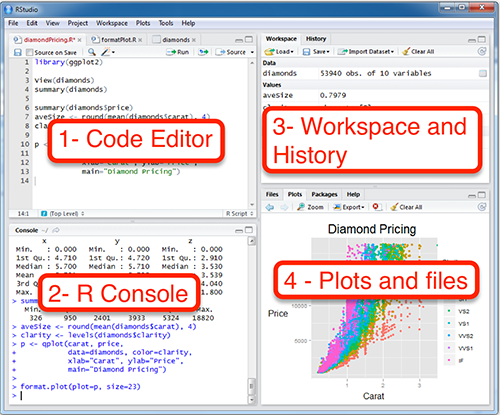
\includegraphics[width=0.8\linewidth]{images/rstudio_layout} \caption{From: http://www.sthda.com/english/wiki/r-basics-quick-and-easy }\label{fig:unnamed-chunk-3}
\end{figure}

\begin{enumerate}
\def\labelenumi{\arabic{enumi}.}
\item
  \textbf{Code Editor/ R script:} Here you can write either R code , or Rmarkdown. That is we can include instructions for our computer to execute.
\item
  \textbf{R console :} Here you see the output of the code you run , if you write code here, it will automatically be run after \texttt{enter} and cannot be traced back, that is why the R Script is useful for reusable code.
\item
  \textbf{Workspace and history: } This space display the variables created , in use, the history , building , git and more. To check if your data has been loaded correctly you can check here to see it loaded.
\item
  \textbf{Plots and files: } It will display the graphs and plots created, you can switch back and forth , export, save and more. Also, you can select packages, get help on \texttt{R} functions and more.
\end{enumerate}

\subsubsection*{What are packages?}\label{what-are-packages}
\addcontentsline{toc}{subsubsection}{What are packages?}

The power of R lies in the packages. Since \texttt{R} is open source, many people create packages i.e, R scripts that contain functions for specific problems , may it be standard deviation , statistics, machine learning and more.

\begin{itemize}
\tightlist
\item
  To install a package, simply type
\end{itemize}

\texttt{install.packages("package\ name")}

\begin{itemize}
\item
  Install a package from Bioconductor: \texttt{biocLite()}
\item
  Install a package from GitHub: \texttt{devtools::install\_github()}
\item
  View the list of installed packages: \texttt{installed.packages()}
\item
  Folder containing installed packages: \texttt{.libPaths()}
\item
  To load a package
\end{itemize}

\texttt{library(package\ name)}

\begin{itemize}
\tightlist
\item
  View loaded packages
\end{itemize}

\texttt{search()}

\begin{itemize}
\tightlist
\item
  to Unload an R package:
\end{itemize}

\texttt{detach(package\ name,\ unload\ =\ TRUE)}

\begin{itemize}
\tightlist
\item
  Remove installed packages:
\end{itemize}

\texttt{remove.packages()}

\begin{itemize}
\tightlist
\item
  Update installed packages:
\end{itemize}

\texttt{update.packages()}

\chapter*{Part II: R Fundamentals}\label{part-ii-r-fundamentals}
\addcontentsline{toc}{chapter}{Part II: R Fundamentals}

Before starting, here are some Official manuals and books we will be learning from:

\begin{enumerate}
\def\labelenumi{\arabic{enumi}.}
\tightlist
\item
  \url{https://cran.r-project.org/doc/manuals/r-release/R-intro.html} \citep{RIntro}
\item
  \url{https://cran.r-project.org/doc/manuals/r-release/R-data.html} \citep{RData}
\item
  \url{https://cran.r-project.org/doc/manuals/r-release/R-exts.html} \citep{RExts}
\item
  \url{https://cran.r-project.org/doc/manuals/r-release/R-lang.html} \citep{RLang}
\item
  \href{https://bookdown.org/rdpeng/rprogdatascience/}{R programming for Data Science by Roger D. Peng.} \citep{Peng2024}
\item
  \href{https://r4ds.had.co.nz/}{R for Data Science} \citep{WickhamHadley2024}
\item
  \href{https://katrienantonio.github.io/intro-R-book/}{Intro R book} \citep{Antonio2020}
\item
  \href{https://unl-statistics.github.io/R-workshops/}{R workshop} \citep{UNLWorkshops}
\item
  \href{https://intro2r.com/}{Intro to R} \citep{Intro2R2024}
\end{enumerate}

\subsection*{R as a calculator}\label{r-as-a-calculator}
\addcontentsline{toc}{subsection}{R as a calculator}

The best way to get used to R is to use it as a calculator.

You can start by using the R console and doing simple operations.

\subsection*{Basic arithmetic operations}\label{basic-arithmetic-operations}
\addcontentsline{toc}{subsection}{Basic arithmetic operations}

\begin{itemize}
\tightlist
\item
  Addition
\end{itemize}

\begin{Shaded}
\begin{Highlighting}[]
\DecValTok{3}\SpecialCharTok{+}\DecValTok{5}
\CommentTok{\#\textgreater{} [1] 8}
\end{Highlighting}
\end{Shaded}

\begin{itemize}
\tightlist
\item
  Subtraction
\end{itemize}

\begin{Shaded}
\begin{Highlighting}[]
\DecValTok{143{-}12}
\CommentTok{\#\textgreater{} [1] 131}
\end{Highlighting}
\end{Shaded}

\begin{itemize}
\tightlist
\item
  Multiplication
\end{itemize}

\begin{Shaded}
\begin{Highlighting}[]
\DecValTok{4}\SpecialCharTok{*}\DecValTok{5}
\CommentTok{\#\textgreater{} [1] 20}
\end{Highlighting}
\end{Shaded}

\begin{itemize}
\tightlist
\item
  Division
\end{itemize}

\begin{Shaded}
\begin{Highlighting}[]
\DecValTok{180}\SpecialCharTok{/}\DecValTok{23}
\CommentTok{\#\textgreater{} [1] 7.826087}
\end{Highlighting}
\end{Shaded}

\begin{itemize}
\tightlist
\item
  Exponientiation
\end{itemize}

\begin{Shaded}
\begin{Highlighting}[]
\DecValTok{4}\SpecialCharTok{\^{}}\DecValTok{2}
\CommentTok{\#\textgreater{} [1] 16}
\end{Highlighting}
\end{Shaded}

\subsubsection*{Arithmetic Functions}\label{arithmetic-functions}
\addcontentsline{toc}{subsubsection}{Arithmetic Functions}

this functions may be useful to replace your calculator

\begin{itemize}
\tightlist
\item
  Absolute value
\end{itemize}

\begin{Shaded}
\begin{Highlighting}[]
\FunctionTok{abs}\NormalTok{(}\SpecialCharTok{{-}}\DecValTok{23}\NormalTok{)}
\CommentTok{\#\textgreater{} [1] 23}
\end{Highlighting}
\end{Shaded}

\begin{itemize}
\tightlist
\item
  Square root
\end{itemize}

\begin{Shaded}
\begin{Highlighting}[]
\FunctionTok{sqrt}\NormalTok{(}\DecValTok{16}\NormalTok{)}
\CommentTok{\#\textgreater{} [1] 4}
\end{Highlighting}
\end{Shaded}

\begin{itemize}
\tightlist
\item
  Remainder/modulo
\end{itemize}

\begin{Shaded}
\begin{Highlighting}[]
\DecValTok{7} \SpecialCharTok{\%\%} \DecValTok{3}
\CommentTok{\#\textgreater{} [1] 1}
\end{Highlighting}
\end{Shaded}

\begin{itemize}
\tightlist
\item
  Logarithms and exponentials
  i.e,
\end{itemize}

\[\log_a b = c,\quad ln_e b=a , \quad  e^{a}=b\]

\begin{Shaded}
\begin{Highlighting}[]
\FunctionTok{log2}\NormalTok{(}\DecValTok{4}\NormalTok{)}
\CommentTok{\#\textgreater{} [1] 2}
\FunctionTok{log10}\NormalTok{(}\DecValTok{1000}\NormalTok{)}
\CommentTok{\#\textgreater{} [1] 3}
\FunctionTok{log}\NormalTok{(}\DecValTok{4}\NormalTok{)}
\CommentTok{\#\textgreater{} [1] 1.386294}
\FunctionTok{exp}\NormalTok{(}\DecValTok{8}\NormalTok{)}
\CommentTok{\#\textgreater{} [1] 2980.958}
\FloatTok{2.71828}\SpecialCharTok{\^{}}\DecValTok{8}
\CommentTok{\#\textgreater{} [1] 2980.942}
\end{Highlighting}
\end{Shaded}

\subsection*{Variables and data types (numeric,character)}\label{variables-and-data-types-numericcharacter}
\addcontentsline{toc}{subsection}{Variables and data types (numeric,character)}

\subsubsection*{Assigment Operators}\label{assigment-operators}
\addcontentsline{toc}{subsubsection}{Assigment Operators}

in \texttt{R}, to create a variable , you can use the assigment symbol \texttt{\textless{}-}, or \texttt{=} however, the later is not commonly used in \texttt{R}.

To assign the value of 7 to x , we will do

\begin{Shaded}
\begin{Highlighting}[]
\NormalTok{x }\OtherTok{\textless{}{-}} \DecValTok{7}
\FunctionTok{print}\NormalTok{(x)}
\CommentTok{\#\textgreater{} [1] 7}
\end{Highlighting}
\end{Shaded}

We can now perform operations on these variables

\begin{Shaded}
\begin{Highlighting}[]
\DecValTok{3}\SpecialCharTok{*}\NormalTok{x}\SpecialCharTok{+}\DecValTok{3} \CommentTok{\# 3*7+3 = 21+3 =24}
\CommentTok{\#\textgreater{} [1] 24}
\end{Highlighting}
\end{Shaded}

\textbf{Remark:} R is case sensitive so, \texttt{x} is different from \texttt{X}

calling \texttt{print(X)} will output error

\begin{Shaded}
\begin{Highlighting}[]
\FunctionTok{print}\NormalTok{(X)}
\CommentTok{\#\textgreater{} Error in eval(expr, envir, enclos): object \textquotesingle{}X\textquotesingle{} not found}
\end{Highlighting}
\end{Shaded}

\subsubsection*{Data types}\label{data-types}
\addcontentsline{toc}{subsubsection}{Data types}

R has five basic or ``atomic'' classes of objects:

\begin{itemize}
\tightlist
\item
  character
\item
  numeric (real numbers)
\item
  integer
\item
  complex
\item
  logical (True/False)
\end{itemize}

\subsubsection*{Exercise 1}\label{exercise-1}
\addcontentsline{toc}{subsubsection}{Exercise 1}

Run the following code, then use typeof(), class() functions to find out the data type and/or class object.

\begin{Shaded}
\begin{Highlighting}[]
\NormalTok{my\_numeric }\OtherTok{\textless{}{-}} \FloatTok{42.5}
\NormalTok{Columbia\_University }\OtherTok{\textless{}{-}} \StringTok{"university"}
\NormalTok{my\_logical }\OtherTok{\textless{}{-}} \ConstantTok{TRUE}
\NormalTok{my\_date }\OtherTok{\textless{}{-}} \FunctionTok{as.Date}\NormalTok{(}\StringTok{"05/29/2018"}\NormalTok{, }\StringTok{"\%m/\%d/\%Y"}\NormalTok{)}
\end{Highlighting}
\end{Shaded}

Use \texttt{typeof()} or \texttt{class()}function to find out what the data type of a variable is .

\subsubsection*{What is the difference between typeof() and class()?}\label{what-is-the-difference-between-typeof-and-class}
\addcontentsline{toc}{subsubsection}{What is the difference between typeof() and class()?}

Here we can see that \texttt{typeof(my\_date)} is a double, and \texttt{class(my\_date)} is \texttt{Date}. This is because \texttt{typeof} output the lowest level data type of the object. While \texttt{class} outputs the class of the object.

If you are writing code that involves checking whether an element is of an specific data type , then you need to be careful on how you check that. Depending on the function , it may give you a true value when in reality you want a false value to be returned.

For example, Imagine you are asked to check if all dates in a dateframe have the correct data type.

In some cases it might be \texttt{"05/29/2018"} but in a rare case (maybe due to a data entry error), there is a \texttt{"42.5"}

\begin{Shaded}
\begin{Highlighting}[]
\FunctionTok{typeof}\NormalTok{(my\_date) }\SpecialCharTok{==} \FunctionTok{typeof}\NormalTok{(my\_numeric)}
\CommentTok{\#\textgreater{} [1] TRUE}
\end{Highlighting}
\end{Shaded}

In the previous comparison , it returns true, meaning that the two data types are the same, maybe youu thought you are comparing if both are date type, but in reality , you are comparing the lowest level data types which are indeed equal (double)

Instead, you should do.

\begin{Shaded}
\begin{Highlighting}[]
\FunctionTok{class}\NormalTok{(my\_date) }\SpecialCharTok{==} \FunctionTok{class}\NormalTok{(my\_numeric)}
\CommentTok{\#\textgreater{} [1] FALSE}
\end{Highlighting}
\end{Shaded}

\textbf{Character Data type }
A character stores character values or strings

\begin{Shaded}
\begin{Highlighting}[]
\NormalTok{char }\OtherTok{\textless{}{-}} \StringTok{"This is a character data type"}
\NormalTok{char}
\CommentTok{\#\textgreater{} [1] "This is a character data type"}
\FunctionTok{typeof}\NormalTok{(char)}
\CommentTok{\#\textgreater{} [1] "character"}
\end{Highlighting}
\end{Shaded}

\textbf{Numeric Data type }

This is for numerical values .

\begin{Shaded}
\begin{Highlighting}[]
\NormalTok{num }\OtherTok{\textless{}{-}} \DecValTok{3}
\FunctionTok{print}\NormalTok{(num)}
\CommentTok{\#\textgreater{} [1] 3}
\NormalTok{num\_2 }\OtherTok{\textless{}{-}} \SpecialCharTok{{-}}\FloatTok{2.35}
\NormalTok{num\_2}
\CommentTok{\#\textgreater{} [1] {-}2.35}
\FunctionTok{typeof}\NormalTok{(num\_2)}
\CommentTok{\#\textgreater{} [1] "double"}
\FunctionTok{class}\NormalTok{(num\_2)}
\CommentTok{\#\textgreater{} [1] "numeric"}
\end{Highlighting}
\end{Shaded}

\textbf{Integer Data type}

For integers, we must specify it as so, and to do it , we must convert the data type. Remark: if it is a decimal, it will remove all decimal, acting as a floor function .

\begin{Shaded}
\begin{Highlighting}[]
\NormalTok{int }\OtherTok{\textless{}{-}} \FunctionTok{as.integer}\NormalTok{(}\FloatTok{3.6332}\NormalTok{)}
\NormalTok{int}
\CommentTok{\#\textgreater{} [1] 3}
\FunctionTok{typeof}\NormalTok{(int)}
\CommentTok{\#\textgreater{} [1] "integer"}
\NormalTok{int2 }\OtherTok{\textless{}{-}} \FunctionTok{as.integer}\NormalTok{(}\DecValTok{7}\NormalTok{)}
\NormalTok{int2}
\CommentTok{\#\textgreater{} [1] 7}
\FunctionTok{typeof}\NormalTok{(int2)}
\CommentTok{\#\textgreater{} [1] "integer"}
\FunctionTok{class}\NormalTok{(int2)}
\CommentTok{\#\textgreater{} [1] "integer"}
\end{Highlighting}
\end{Shaded}

We can also create a integer by adding an L after it

\begin{Shaded}
\begin{Highlighting}[]
\NormalTok{int3 }\OtherTok{\textless{}{-}} \DecValTok{8}\DataTypeTok{L}
\NormalTok{int3}
\CommentTok{\#\textgreater{} [1] 8}
\end{Highlighting}
\end{Shaded}

Remark: It does not work with decimals

\begin{Shaded}
\begin{Highlighting}[]
\NormalTok{int4 }\OtherTok{\textless{}{-}} \FloatTok{3.4546}\NormalTok{L}
\NormalTok{int4}
\CommentTok{\#\textgreater{} [1] 3.4546}
\end{Highlighting}
\end{Shaded}

\textbf{Complex Data type}
Complex data types are stored as \texttt{x+yi} , i.e, with the imaginary component

\begin{Shaded}
\begin{Highlighting}[]
\NormalTok{compl }\OtherTok{\textless{}{-}} \DecValTok{13}\SpecialCharTok{+}\DecValTok{7}\DataTypeTok{i}
\NormalTok{compl}
\CommentTok{\#\textgreater{} [1] 13+7i}
\FunctionTok{typeof}\NormalTok{(compl)}
\CommentTok{\#\textgreater{} [1] "complex"}
\FunctionTok{complex}\NormalTok{(}\AttributeTok{real =} \DecValTok{23}\NormalTok{, }\AttributeTok{imaginary =} \DecValTok{7}\NormalTok{)}
\CommentTok{\#\textgreater{} [1] 23+7i}
\end{Highlighting}
\end{Shaded}

\textbf{Boolean Data type }
This stores boolean values of \texttt{TRUE} and \texttt{FALSE}

\begin{Shaded}
\begin{Highlighting}[]
\NormalTok{my\_bool }\OtherTok{\textless{}{-}} \ConstantTok{TRUE}
\NormalTok{my\_bool}
\CommentTok{\#\textgreater{} [1] TRUE}

\FunctionTok{typeof}\NormalTok{(my\_bool)}
\CommentTok{\#\textgreater{} [1] "logical"}

\NormalTok{my\_boolean }\OtherTok{\textless{}{-}}\NormalTok{ F}
\NormalTok{my\_boolean}
\CommentTok{\#\textgreater{} [1] FALSE}
\FunctionTok{typeof}\NormalTok{(my\_boolean)}
\CommentTok{\#\textgreater{} [1] "logical"}
\end{Highlighting}
\end{Shaded}

\subsubsection*{Converting Data types}\label{converting-data-types}
\addcontentsline{toc}{subsubsection}{Converting Data types}

\textbf{Convert into Numeric}

We can convert values as numeric. Using \texttt{as.numeric()} to change the type but keeping the values as they are.
When converting

\begin{itemize}
\tightlist
\item
  complex: removes the \texttt{imaginary} part
\item
  logical: \texttt{TRUE} becomes \texttt{1} , \texttt{FALSE} becomes \texttt{0}
\item
  character: to its numerical values, but if it has letters then to \texttt{NA}
\end{itemize}

We can use \texttt{is.numeric()} to check if a variable is numeric

\begin{Shaded}
\begin{Highlighting}[]
\CommentTok{\# Complex}
\FunctionTok{is.numeric}\NormalTok{(compl)}
\CommentTok{\#\textgreater{} [1] FALSE}
\NormalTok{number }\OtherTok{\textless{}{-}} \FunctionTok{as.numeric}\NormalTok{(compl)}
\CommentTok{\#\textgreater{} Warning: imaginary parts discarded in coercion}
\NormalTok{number}
\CommentTok{\#\textgreater{} [1] 13}
\FunctionTok{is.numeric}\NormalTok{(number)}
\CommentTok{\#\textgreater{} [1] TRUE}

\CommentTok{\#Logical }
\FunctionTok{is.numeric}\NormalTok{(my\_bool)}
\CommentTok{\#\textgreater{} [1] FALSE}
\NormalTok{number2 }\OtherTok{\textless{}{-}} \FunctionTok{as.numeric}\NormalTok{(my\_bool)}
\NormalTok{number2}
\CommentTok{\#\textgreater{} [1] 1}
\FunctionTok{is.numeric}\NormalTok{(number2)}
\CommentTok{\#\textgreater{} [1] TRUE}

\CommentTok{\# Character}
\NormalTok{char}
\CommentTok{\#\textgreater{} [1] "This is a character data type"}
\FunctionTok{is.numeric}\NormalTok{(char)}
\CommentTok{\#\textgreater{} [1] FALSE}
\NormalTok{number3 }\OtherTok{\textless{}{-}} \FunctionTok{as.numeric}\NormalTok{(char)}
\CommentTok{\#\textgreater{} Warning: NAs introduced by coercion}
\NormalTok{number3}
\CommentTok{\#\textgreater{} [1] NA}
\FunctionTok{is.numeric}\NormalTok{(number3)}
\CommentTok{\#\textgreater{} [1] TRUE}

\NormalTok{my\_char }\OtherTok{\textless{}{-}} \StringTok{"2023"}
\FunctionTok{is.numeric}\NormalTok{(my\_char)}
\CommentTok{\#\textgreater{} [1] FALSE}
\NormalTok{number4 }\OtherTok{\textless{}{-}} \FunctionTok{as.numeric}\NormalTok{(my\_char)}
\NormalTok{number4}
\CommentTok{\#\textgreater{} [1] 2023}
\FunctionTok{is.numeric}\NormalTok{(number4)}
\CommentTok{\#\textgreater{} [1] TRUE}
\end{Highlighting}
\end{Shaded}

\textbf{Convert into integer}

\begin{Shaded}
\begin{Highlighting}[]
\NormalTok{inte1}\OtherTok{\textless{}{-}}\FunctionTok{as.integer}\NormalTok{(}\StringTok{"234"}\NormalTok{)}
\NormalTok{inte1}
\CommentTok{\#\textgreater{} [1] 234}
\FunctionTok{typeof}\NormalTok{(inte1)}
\CommentTok{\#\textgreater{} [1] "integer"}

\NormalTok{inte2}\OtherTok{\textless{}{-}}\FunctionTok{as.integer}\NormalTok{(}\DecValTok{23}\SpecialCharTok{+}\DecValTok{6}\DataTypeTok{i}\NormalTok{)}
\CommentTok{\#\textgreater{} Warning: imaginary parts discarded in coercion}
\NormalTok{inte2}
\CommentTok{\#\textgreater{} [1] 23}
\FunctionTok{typeof}\NormalTok{(inte2)}
\CommentTok{\#\textgreater{} [1] "integer"}

\NormalTok{inte3}\OtherTok{\textless{}{-}}\FunctionTok{as.integer}\NormalTok{(F)}
\NormalTok{inte3}
\CommentTok{\#\textgreater{} [1] 0}
\FunctionTok{typeof}\NormalTok{(inte3)}
\CommentTok{\#\textgreater{} [1] "integer"}
\end{Highlighting}
\end{Shaded}

\textbf{Converting into Logical}

Return \texttt{FALSE} for \texttt{0} , \texttt{TRUE} otherwise

\begin{Shaded}
\begin{Highlighting}[]
\FunctionTok{print}\NormalTok{(}\FunctionTok{as.logical}\NormalTok{(}\DecValTok{0}\NormalTok{))}
\CommentTok{\#\textgreater{} [1] FALSE}
\FunctionTok{typeof}\NormalTok{(}\FunctionTok{as.logical}\NormalTok{(}\DecValTok{0}\NormalTok{))}
\CommentTok{\#\textgreater{} [1] "logical"}

\FunctionTok{print}\NormalTok{(}\FunctionTok{as.logical}\NormalTok{(}\SpecialCharTok{{-}}\DecValTok{324}\NormalTok{))}
\CommentTok{\#\textgreater{} [1] TRUE}
\FunctionTok{typeof}\NormalTok{(}\FunctionTok{as.logical}\NormalTok{(}\SpecialCharTok{{-}}\DecValTok{324}\NormalTok{))}
\CommentTok{\#\textgreater{} [1] "logical"}
\end{Highlighting}
\end{Shaded}

\subsubsection*{Exercise 2}\label{exercise-2}
\addcontentsline{toc}{subsubsection}{Exercise 2}

Create 1 datatype of each: Character, numeric, integer, complex, Boolean

\subsection*{Getting help}\label{getting-help}
\addcontentsline{toc}{subsection}{Getting help}

You can use the Plots and files pane (bottom left pane) to click on Help and then search for whichever function you need help with.

You can also use the \texttt{?} before each function.

\begin{Shaded}
\begin{Highlighting}[]
\NormalTok{?mean}
\end{Highlighting}
\end{Shaded}

This will open the information about the function on the plots and files pane.

\chapter*{Part III: Data Structures}\label{part-iii-data-structures}
\addcontentsline{toc}{chapter}{Part III: Data Structures}

\section*{Vectors: Creating, indexing, and operations}\label{vectors-creating-indexing-and-operations}
\addcontentsline{toc}{section}{Vectors: Creating, indexing, and operations}

\begin{Shaded}
\begin{Highlighting}[]
\CommentTok{\# Creating a vector}
\NormalTok{v }\OtherTok{\textless{}{-}} \FunctionTok{c}\NormalTok{(}\DecValTok{1}\NormalTok{, }\DecValTok{2}\NormalTok{, }\DecValTok{3}\NormalTok{, }\DecValTok{4}\NormalTok{, }\DecValTok{5}\NormalTok{)}
\FunctionTok{print}\NormalTok{(v)}
\CommentTok{\#\textgreater{} [1] 1 2 3 4 5}

\CommentTok{\# Indexing a vector}
\FunctionTok{print}\NormalTok{(v[}\DecValTok{2}\NormalTok{])  }\CommentTok{\# Access the second element}
\CommentTok{\#\textgreater{} [1] 2}

\CommentTok{\# Vector operations}
\NormalTok{v2 }\OtherTok{\textless{}{-}}\NormalTok{ v }\SpecialCharTok{*} \DecValTok{2}  \CommentTok{\# Multiply each element by 2}
\FunctionTok{print}\NormalTok{(v2)}
\CommentTok{\#\textgreater{} [1]  2  4  6  8 10}
\end{Highlighting}
\end{Shaded}

You can give names to the columns of the vector

\begin{Shaded}
\begin{Highlighting}[]
\NormalTok{my\_vector }\OtherTok{\textless{}{-}} \FunctionTok{c}\NormalTok{(}\StringTok{"Dilan Caro"}\NormalTok{, }\StringTok{"Instructor"}\NormalTok{)}
\FunctionTok{names}\NormalTok{(my\_vector) }\OtherTok{\textless{}{-}} \FunctionTok{c}\NormalTok{(}\StringTok{"Name"}\NormalTok{, }\StringTok{"Profession"}\NormalTok{)}
\NormalTok{my\_vector}
\CommentTok{\#\textgreater{}         Name   Profession }
\CommentTok{\#\textgreater{} "Dilan Caro" "Instructor"}
\end{Highlighting}
\end{Shaded}

\subsection*{Exercise 1:}\label{exercise-1-1}
\addcontentsline{toc}{subsection}{Exercise 1:}

\begin{enumerate}
\def\labelenumi{\arabic{enumi}.}
\tightlist
\item
  Create a vector of your favorite numbers.
\item
  Access the third element in your vector.
\item
  Create a new vector that is the square of each element in the original vector.
\end{enumerate}

\begin{Shaded}
\begin{Highlighting}[]
\NormalTok{my\_vector }\OtherTok{\textless{}{-}} \FunctionTok{c}\NormalTok{(}\StringTok{"Dilan Caro"}\NormalTok{, }\StringTok{"Instructor"}\NormalTok{)}
\FunctionTok{names}\NormalTok{(my\_vector) }\OtherTok{\textless{}{-}} \FunctionTok{c}\NormalTok{(}\StringTok{"Name"}\NormalTok{, }\StringTok{"Profession"}\NormalTok{)}
\NormalTok{my\_vector}
\CommentTok{\#\textgreater{}         Name   Profession }
\CommentTok{\#\textgreater{} "Dilan Caro" "Instructor"}
\end{Highlighting}
\end{Shaded}

\begin{enumerate}
\def\labelenumi{\arabic{enumi}.}
\setcounter{enumi}{3}
\tightlist
\item
  Inspect my\_vector using:
  the attributes(), the length() and the str() function
\end{enumerate}

\section*{Matrices}\label{matrices}
\addcontentsline{toc}{section}{Matrices}

Matrices are vectors with a dimension attribute. The dimension attribute is itself an integer vector of length 2 (number of rows, number of columns)

Matrices are constructed column-wise, so entries can be thought of starting in the ``upper left'' corner and running down the columns.

\begin{Shaded}
\begin{Highlighting}[]
\NormalTok{m }\OtherTok{\textless{}{-}} \FunctionTok{matrix}\NormalTok{(}\DecValTok{1}\SpecialCharTok{:}\DecValTok{6}\NormalTok{, }\AttributeTok{nrow =} \DecValTok{2}\NormalTok{, }\AttributeTok{ncol =} \DecValTok{3}\NormalTok{) }
\NormalTok{m}
\CommentTok{\#\textgreater{}      [,1] [,2] [,3]}
\CommentTok{\#\textgreater{} [1,]    1    3    5}
\CommentTok{\#\textgreater{} [2,]    2    4    6}
\end{Highlighting}
\end{Shaded}

Another example

\begin{Shaded}
\begin{Highlighting}[]
\NormalTok{my\_matrix }\OtherTok{\textless{}{-}} \FunctionTok{matrix}\NormalTok{(}\DecValTok{1}\SpecialCharTok{:}\DecValTok{12}\NormalTok{, }\DecValTok{3}\NormalTok{, }\DecValTok{4}\NormalTok{, }\AttributeTok{byrow =} \ConstantTok{TRUE}\NormalTok{)}
\NormalTok{my\_matrix}
\CommentTok{\#\textgreater{}      [,1] [,2] [,3] [,4]}
\CommentTok{\#\textgreater{} [1,]    1    2    3    4}
\CommentTok{\#\textgreater{} [2,]    5    6    7    8}
\CommentTok{\#\textgreater{} [3,]    9   10   11   12}
\end{Highlighting}
\end{Shaded}

Matrices can be created by column-binding or row-binding with the \texttt{cbind()} and \texttt{rbind()} functions.

\begin{Shaded}
\begin{Highlighting}[]
\NormalTok{x }\OtherTok{\textless{}{-}} \DecValTok{1}\SpecialCharTok{:}\DecValTok{3}
\NormalTok{y }\OtherTok{\textless{}{-}} \DecValTok{10}\SpecialCharTok{:}\DecValTok{12}
\FunctionTok{cbind}\NormalTok{(x, y)}
\CommentTok{\#\textgreater{}      x  y}
\CommentTok{\#\textgreater{} [1,] 1 10}
\CommentTok{\#\textgreater{} [2,] 2 11}
\CommentTok{\#\textgreater{} [3,] 3 12}
\FunctionTok{rbind}\NormalTok{(x, y)}
\CommentTok{\#\textgreater{}   [,1] [,2] [,3]}
\CommentTok{\#\textgreater{} x    1    2    3}
\CommentTok{\#\textgreater{} y   10   11   12}
\end{Highlighting}
\end{Shaded}

\section*{Seq and rep functions}\label{seq-and-rep-functions}
\addcontentsline{toc}{section}{Seq and rep functions}

In R, seq and rep are two functions used to generate sequences and to replicate values, respectively.

\subsection{\texorpdfstring{\texttt{seq} Function:}{seq Function:}}\label{seq-function}

The seq function is used to create a sequence of numbers.

Usage:

\begin{itemize}
\item
  seq(from, to): Generates a sequence from the `from' value to the `to' value with a default increment of 1.
\item
  seq(from, to, by): Generates a sequence from the `from' value to the `to' value, with the increment specified by `by'.
\item
  seq(from, to, length.out): Generates a sequence from the `from' value to the `to' value with a specified number of equally spaced points.
\end{itemize}

\subsubsection*{Example}\label{example}
\addcontentsline{toc}{subsubsection}{Example}

\begin{Shaded}
\begin{Highlighting}[]
\FunctionTok{seq}\NormalTok{(}\DecValTok{1}\NormalTok{, }\DecValTok{5}\NormalTok{)         }
\CommentTok{\#\textgreater{} [1] 1 2 3 4 5}
\FunctionTok{seq}\NormalTok{(}\DecValTok{1}\NormalTok{, }\DecValTok{10}\NormalTok{, }\AttributeTok{by =} \DecValTok{2}\NormalTok{)    }
\CommentTok{\#\textgreater{} [1] 1 3 5 7 9}
\FunctionTok{seq}\NormalTok{(}\DecValTok{1}\NormalTok{, }\DecValTok{10}\NormalTok{, }\AttributeTok{length.out =} \DecValTok{4}\NormalTok{) }
\CommentTok{\#\textgreater{} [1]  1  4  7 10}
\end{Highlighting}
\end{Shaded}

\subsection{\texorpdfstring{\texttt{rep} Function:}{rep Function:}}\label{rep-function}

The rep function is used to replicate the values in a vector.

Usage:

\begin{itemize}
\item
  rep(x, times): Replicates each element in `x' a specified number of `times'.
\item
  rep(x, each): Replicates each element in `x' `each' times before moving to the next element.
\item
  rep(x, length.out): Replicates the values in `x' up to the `length.out' number of times in total.
\end{itemize}

\begin{Shaded}
\begin{Highlighting}[]
\FunctionTok{rep}\NormalTok{(}\DecValTok{1}\SpecialCharTok{:}\DecValTok{3}\NormalTok{, }\AttributeTok{times =} \DecValTok{2}\NormalTok{)}
\CommentTok{\#\textgreater{} [1] 1 2 3 1 2 3}
\FunctionTok{rep}\NormalTok{(}\DecValTok{1}\SpecialCharTok{:}\DecValTok{3}\NormalTok{, }\AttributeTok{each =} \DecValTok{2}\NormalTok{)       }
\CommentTok{\#\textgreater{} [1] 1 1 2 2 3 3}
\FunctionTok{rep}\NormalTok{(}\DecValTok{1}\SpecialCharTok{:}\DecValTok{3}\NormalTok{, }\AttributeTok{length.out =} \DecValTok{7}\NormalTok{)   }
\CommentTok{\#\textgreater{} [1] 1 2 3 1 2 3 1}
\end{Highlighting}
\end{Shaded}

\section*{Lists}\label{lists}
\addcontentsline{toc}{section}{Lists}

Lists are a special type of vector that can contain elements of different classes. Lists are a very important data type in R and you should get to know them well. Lists, in combination with the various ``apply'' functions discussed later, make for a powerful combination.

Lists can be explicitly created using the list() function, which takes an arbitrary number of arguments.

\begin{Shaded}
\begin{Highlighting}[]
\NormalTok{x }\OtherTok{\textless{}{-}} \FunctionTok{list}\NormalTok{(}\DecValTok{1}\NormalTok{, }\StringTok{"a"}\NormalTok{, }\ConstantTok{TRUE}\NormalTok{, }\DecValTok{1} \SpecialCharTok{+} \DecValTok{4}\DataTypeTok{i}\NormalTok{) }
\NormalTok{x}
\CommentTok{\#\textgreater{} [[1]]}
\CommentTok{\#\textgreater{} [1] 1}
\CommentTok{\#\textgreater{} }
\CommentTok{\#\textgreater{} [[2]]}
\CommentTok{\#\textgreater{} [1] "a"}
\CommentTok{\#\textgreater{} }
\CommentTok{\#\textgreater{} [[3]]}
\CommentTok{\#\textgreater{} [1] TRUE}
\CommentTok{\#\textgreater{} }
\CommentTok{\#\textgreater{} [[4]]}
\CommentTok{\#\textgreater{} [1] 1+4i}
\end{Highlighting}
\end{Shaded}

\subsection*{Example}\label{example-1}
\addcontentsline{toc}{subsection}{Example}

\begin{Shaded}
\begin{Highlighting}[]
\NormalTok{my\_list }\OtherTok{\textless{}{-}} \FunctionTok{list}\NormalTok{(}\AttributeTok{one =} \DecValTok{1}\NormalTok{, }\AttributeTok{two =} \FunctionTok{c}\NormalTok{(}\DecValTok{1}\NormalTok{, }\DecValTok{2}\NormalTok{), }\AttributeTok{five =} \FunctionTok{seq}\NormalTok{(}\DecValTok{1}\NormalTok{, }\DecValTok{4}\NormalTok{, }\AttributeTok{length=}\DecValTok{5}\NormalTok{),}
          \AttributeTok{six =} \FunctionTok{c}\NormalTok{(}\StringTok{"Dilan"}\NormalTok{, }\StringTok{"April"}\NormalTok{))}
\FunctionTok{names}\NormalTok{(my\_list)}
\CommentTok{\#\textgreater{} [1] "one"  "two"  "five" "six"}
\end{Highlighting}
\end{Shaded}

\begin{Shaded}
\begin{Highlighting}[]
\FunctionTok{str}\NormalTok{(my\_list)}
\CommentTok{\#\textgreater{} List of 4}
\CommentTok{\#\textgreater{}  $ one : num 1}
\CommentTok{\#\textgreater{}  $ two : num [1:2] 1 2}
\CommentTok{\#\textgreater{}  $ five: num [1:5] 1 1.75 2.5 3.25 4}
\CommentTok{\#\textgreater{}  $ six : chr [1:2] "Dilan" "April"}
\end{Highlighting}
\end{Shaded}

\section*{Factors}\label{factors}
\addcontentsline{toc}{section}{Factors}

Factors are used to represent categorical data and can be unordered or ordered. One can think of a factor as an integer vector where each integer has a label. Factors are important in statistical modeling and are treated specially by modelling functions like \texttt{lm()} and \texttt{glm()}.

Using factors with labels is better than using integers because factors are self-describing. Having a variable that has values ``Male'' and ``Female'' is better than a variable that has values 1 and 2.

Factor objects can be created with the factor() function.

\begin{Shaded}
\begin{Highlighting}[]
\NormalTok{x }\OtherTok{\textless{}{-}} \FunctionTok{factor}\NormalTok{(}\FunctionTok{c}\NormalTok{(}\StringTok{"yes"}\NormalTok{, }\StringTok{"yes"}\NormalTok{, }\StringTok{"no"}\NormalTok{, }\StringTok{"yes"}\NormalTok{, }\StringTok{"no"}\NormalTok{)) }
\NormalTok{x}
\CommentTok{\#\textgreater{} [1] yes yes no  yes no }
\CommentTok{\#\textgreater{} Levels: no yes}
\end{Highlighting}
\end{Shaded}

Level are put in alphabetical order, but you can also define the levels.

\begin{Shaded}
\begin{Highlighting}[]
\NormalTok{x }\OtherTok{\textless{}{-}} \FunctionTok{factor}\NormalTok{(}\FunctionTok{c}\NormalTok{(}\StringTok{"yes"}\NormalTok{, }\StringTok{"yes"}\NormalTok{, }\StringTok{"no"}\NormalTok{, }\StringTok{"yes"}\NormalTok{, }\StringTok{"no"}\NormalTok{),}\AttributeTok{levels =} \FunctionTok{c}\NormalTok{(}\StringTok{"yes"}\NormalTok{, }\StringTok{"no"}\NormalTok{))}
\NormalTok{x}
\CommentTok{\#\textgreater{} [1] yes yes no  yes no }
\CommentTok{\#\textgreater{} Levels: yes no}
\end{Highlighting}
\end{Shaded}

\section*{Data frames: Creating and exploring data frames}\label{data-frames-creating-and-exploring-data-frames}
\addcontentsline{toc}{section}{Data frames: Creating and exploring data frames}

Data frames are used to store tabular data in R.

Data frames are represented as a special type of list where every element of the list has to have the same length. Each element of the list can be thought of as a column and the length of each element of the list is the number of rows.

\begin{Shaded}
\begin{Highlighting}[]
\CommentTok{\# Creating a data frame}
\NormalTok{df }\OtherTok{\textless{}{-}} \FunctionTok{data.frame}\NormalTok{(}
  \AttributeTok{Name =} \FunctionTok{c}\NormalTok{(}\StringTok{"Alice"}\NormalTok{, }\StringTok{"Bob"}\NormalTok{, }\StringTok{"Charlie"}\NormalTok{),}
  \AttributeTok{Age =} \FunctionTok{c}\NormalTok{(}\DecValTok{25}\NormalTok{, }\DecValTok{30}\NormalTok{, }\DecValTok{35}\NormalTok{),}
  \AttributeTok{Salary =} \FunctionTok{c}\NormalTok{(}\DecValTok{50000}\NormalTok{, }\DecValTok{60000}\NormalTok{, }\DecValTok{70000}\NormalTok{)}
\NormalTok{)}
\FunctionTok{print}\NormalTok{(df)}
\CommentTok{\#\textgreater{}      Name Age Salary}
\CommentTok{\#\textgreater{} 1   Alice  25  50000}
\CommentTok{\#\textgreater{} 2     Bob  30  60000}
\CommentTok{\#\textgreater{} 3 Charlie  35  70000}

\CommentTok{\# Exploring data frames}
\FunctionTok{print}\NormalTok{(}\FunctionTok{dim}\NormalTok{(df))  }\CommentTok{\# Dimensions of the data frame}
\CommentTok{\#\textgreater{} [1] 3 3}
\FunctionTok{print}\NormalTok{(}\FunctionTok{colnames}\NormalTok{(df))  }\CommentTok{\# Column names}
\CommentTok{\#\textgreater{} [1] "Name"   "Age"    "Salary"}
\FunctionTok{print}\NormalTok{(}\FunctionTok{summary}\NormalTok{(df))  }\CommentTok{\# Summary statistics}
\CommentTok{\#\textgreater{}      Name                Age           Salary     }
\CommentTok{\#\textgreater{}  Length:3           Min.   :25.0   Min.   :50000  }
\CommentTok{\#\textgreater{}  Class :character   1st Qu.:27.5   1st Qu.:55000  }
\CommentTok{\#\textgreater{}  Mode  :character   Median :30.0   Median :60000  }
\CommentTok{\#\textgreater{}                     Mean   :30.0   Mean   :60000  }
\CommentTok{\#\textgreater{}                     3rd Qu.:32.5   3rd Qu.:65000  }
\CommentTok{\#\textgreater{}                     Max.   :35.0   Max.   :70000}
\end{Highlighting}
\end{Shaded}

\subsection*{Exercise 2}\label{exercise-2-1}
\addcontentsline{toc}{subsection}{Exercise 2}

\begin{enumerate}
\def\labelenumi{\arabic{enumi}.}
\tightlist
\item
  Create a data frame with at least three columns and four rows.
\item
  Print the number of rows and columns of your data frame.
\item
  Display summary statistics of your data frame.
\end{enumerate}

\section*{Part 2}\label{part-2}
\addcontentsline{toc}{section}{Part 2}

\subsection*{Exercise 3}\label{exercise-3}
\addcontentsline{toc}{subsection}{Exercise 3}

\begin{enumerate}
\def\labelenumi{\arabic{enumi}.}
\tightlist
\item
  Inspect a built-in data frame, inspect \texttt{mtcars} using \texttt{str()}, \texttt{head()}
\item
  Get summary from a variable in a dataframe, use \texttt{\$} to extract a variable from the dataframe.
\item
  Now inspect a tibble, inspect \texttt{diamonds} from the \texttt{ggplot2} library. Use \texttt{str()}, \texttt{head()}, \texttt{summary()}
\end{enumerate}

\begin{Shaded}
\begin{Highlighting}[]
\NormalTok{mtcars}
\FunctionTok{str}\NormalTok{(mtcars)}
\FunctionTok{head}\NormalTok{(mtcars)}
\end{Highlighting}
\end{Shaded}

\begin{Shaded}
\begin{Highlighting}[]
\FunctionTok{summary}\NormalTok{(mtcars}\SpecialCharTok{$}\NormalTok{cyl) }\CommentTok{\# use $ to extract variable from a data frame}
\end{Highlighting}
\end{Shaded}

\begin{Shaded}
\begin{Highlighting}[]
\FunctionTok{library}\NormalTok{(ggplot2)}
\FunctionTok{head}\NormalTok{(diamonds)}
\end{Highlighting}
\end{Shaded}

Can you list some differences?

\section*{Importing and exporting data (CSV files)}\label{importing-and-exporting-data-csv-files}
\addcontentsline{toc}{section}{Importing and exporting data (CSV files)}

Exporting data to CSV

\begin{Shaded}
\begin{Highlighting}[]
\FunctionTok{write.csv}\NormalTok{(df, }\StringTok{"my\_data.csv"}\NormalTok{, }\AttributeTok{row.names =} \ConstantTok{FALSE}\NormalTok{)}
\end{Highlighting}
\end{Shaded}

Importing data from CSV

\begin{Shaded}
\begin{Highlighting}[]
\NormalTok{df\_imported }\OtherTok{\textless{}{-}} \FunctionTok{read.csv}\NormalTok{(}\StringTok{"my\_data.csv"}\NormalTok{)}
\FunctionTok{print}\NormalTok{(df\_imported)}
\CommentTok{\#\textgreater{}      Name Age Salary}
\CommentTok{\#\textgreater{} 1   Alice  25  50000}
\CommentTok{\#\textgreater{} 2     Bob  30  60000}
\CommentTok{\#\textgreater{} 3 Charlie  35  70000}
\end{Highlighting}
\end{Shaded}

\subsection*{Exercise 4}\label{exercise-4}
\addcontentsline{toc}{subsection}{Exercise 4}

\begin{enumerate}
\def\labelenumi{\arabic{enumi}.}
\tightlist
\item
  Create a vector \texttt{fav\_music} with the names of your favorite artists.
\item
  Create a vector \texttt{num\_records} with the number of records you have in
  your collection of each of those artists.
\item
  Create a vector \texttt{num\_concerts} with the number of times you attended a concert of these artists.
\item
  Put everything together in a data frame, assign the name \texttt{my\_music} to this data frame and change the labels of the information stored in the columns to \texttt{artist}, \texttt{records} and \texttt{concerts.}
\item
  Extract the variable \texttt{num\_records} from the data frame \texttt{my\_music.}
\item
  Calculate the total number of records in your collection (for the defined
  set of artists).
\item
  Check the structure of the data frame, ask for a \texttt{summary.}
\end{enumerate}

Previously, we exported the data and then imported it . Some of you may think, then what is the purpose if we already had the dataframe. The prior was just an example, in reality , you would not have the dataframe loaded in R . You would only have a csv or a data file that a coworker has shared with you or the data engineer has procured for you.

First, we need to obtain the data that we need. For that, please head over to

\url{https://tinyurl.com/STAR-DATA}

The download will automatically start.


\includegraphics[width=0.4\linewidth,height=0.2\textheight]{images/STAR-DATA}

alternatively,

\url{https://download-directory.github.io/?url=https://github.com/DilanCaro/CU-R-Workshop/tree/b6ccfa1f0775ec6c012898175a9f5454ff1063c5/Data}

and download the zip files. If you are unable to download them all, or unzip, download only the necessary files.

Or to individually download the data, please visit.

\url{https://github.com/DilanCaro/CU-R-Workshop/tree/b6ccfa1f0775ec6c012898175a9f5454ff1063c5/Data}

Some useful instructions regarding path names: get your working directory

\begin{itemize}
\tightlist
\item
  Get working directory
\end{itemize}

\begin{Shaded}
\begin{Highlighting}[]
\FunctionTok{getwd}\NormalTok{()}
\CommentTok{\#\textgreater{} [1] "/Users/dilancaro/Library/Mobile Documents/com\textasciitilde{}apple\textasciitilde{}CloudDocs/University/Year 24{-}25/Summer 24/WORK/STAR/CU{-}R{-}Workshop"}
\end{Highlighting}
\end{Shaded}

\begin{itemize}
\tightlist
\item
  specify a path name, with forward slash or double back slash
\end{itemize}

\begin{Shaded}
\begin{Highlighting}[]
\NormalTok{path }\OtherTok{\textless{}{-}} \FunctionTok{file.path}\NormalTok{(}\StringTok{"/Users/dilancaro/Library/Mobile Documents/com\textasciitilde{}apple\textasciitilde{}CloudDocs/University/Year 24{-}25/Summer 24/WORK/STAR/CU R Workshop/Data"}\NormalTok{)}
\end{Highlighting}
\end{Shaded}

\begin{itemize}
\tightlist
\item
  use a relative path
\end{itemize}

\begin{Shaded}
\begin{Highlighting}[]
\NormalTok{path }\OtherTok{\textless{}{-}} \FunctionTok{file.path}\NormalTok{(}\StringTok{"./Data/"}\NormalTok{)}
\end{Highlighting}
\end{Shaded}

\section*{Importing a .txt file}\label{importing-a-.txt-file}
\addcontentsline{toc}{section}{Importing a .txt file}

\texttt{read.table()} is one great way to import data.

\begin{Shaded}
\begin{Highlighting}[]

\NormalTok{path.hotdogs }\OtherTok{\textless{}{-}} \FunctionTok{file.path}\NormalTok{(path, }\StringTok{"hotdogs.txt"}\NormalTok{)}
\NormalTok{path.hotdogs    }\CommentTok{\# inspect path name}
\CommentTok{\#\textgreater{} [1] "./Data//hotdogs.txt"}
\NormalTok{hotdogs }\OtherTok{\textless{}{-}} \FunctionTok{read.table}\NormalTok{(path.hotdogs, }\AttributeTok{header =} \ConstantTok{FALSE}\NormalTok{,}
                      \AttributeTok{col.names =} \FunctionTok{c}\NormalTok{(}\StringTok{"type"}\NormalTok{, }\StringTok{"calories"}\NormalTok{, }\StringTok{"sodium"}\NormalTok{))}
\FunctionTok{str}\NormalTok{(hotdogs)    }\CommentTok{\# inspect data imported}
\CommentTok{\#\textgreater{} \textquotesingle{}data.frame\textquotesingle{}:    54 obs. of  3 variables:}
\CommentTok{\#\textgreater{}  $ type    : chr  "Beef" "Beef" "Beef" "Beef" ...}
\CommentTok{\#\textgreater{}  $ calories: int  186 181 176 149 184 190 158 139 175 148 ...}
\CommentTok{\#\textgreater{}  $ sodium  : int  495 477 425 322 482 587 370 322 479 375 ...}
\end{Highlighting}
\end{Shaded}

Or like this

\begin{Shaded}
\begin{Highlighting}[]
\NormalTok{hotdogs2 }\OtherTok{\textless{}{-}} \FunctionTok{read.table}\NormalTok{(path.hotdogs, }\AttributeTok{header =} \ConstantTok{FALSE}\NormalTok{,}
                       \AttributeTok{col.names =} \FunctionTok{c}\NormalTok{(}\StringTok{"type"}\NormalTok{, }\StringTok{"calories"}\NormalTok{, }\StringTok{"sodium"}\NormalTok{),}
                       \AttributeTok{colClasses =} \FunctionTok{c}\NormalTok{(}\StringTok{"factor"}\NormalTok{, }\StringTok{"NULL"}\NormalTok{, }\StringTok{"numeric"}\NormalTok{))}
\FunctionTok{str}\NormalTok{(hotdogs2)}
\CommentTok{\#\textgreater{} \textquotesingle{}data.frame\textquotesingle{}:    54 obs. of  2 variables:}
\CommentTok{\#\textgreater{}  $ type  : Factor w/ 3 levels "Beef","Meat",..: 1 1 1 1 1 1 1 1 1 1 ...}
\CommentTok{\#\textgreater{}  $ sodium: num  495 477 425 322 482 587 370 322 479 375 ...}
\end{Highlighting}
\end{Shaded}

What happened?

\subsection*{Import .csv file}\label{import-.csv-file}
\addcontentsline{toc}{subsection}{Import .csv file}

\texttt{read.csv()} is another importing function.

Here is an example:
- load a data set on swimming pools in Brisbane
- column names in the first row; a comma to separate values within rows

\begin{Shaded}
\begin{Highlighting}[]
\NormalTok{path.pools }\OtherTok{\textless{}{-}} \FunctionTok{file.path}\NormalTok{(path, }\StringTok{"swimming\_pools.csv"}\NormalTok{)}
\NormalTok{pools }\OtherTok{\textless{}{-}} \FunctionTok{read.csv}\NormalTok{(path.pools)}
\FunctionTok{str}\NormalTok{(pools)}
\CommentTok{\#\textgreater{} \textquotesingle{}data.frame\textquotesingle{}:    20 obs. of  4 variables:}
\CommentTok{\#\textgreater{}  $ Name     : chr  "Acacia Ridge Leisure Centre" "Bellbowrie Pool" "Carole Park" "Centenary Pool (inner City)" ...}
\CommentTok{\#\textgreater{}  $ Address  : chr  "1391 Beaudesert Road, Acacia Ridge" "Sugarwood Street, Bellbowrie" "Cnr Boundary Road and Waterford Road Wacol" "400 Gregory Terrace, Spring Hill" ...}
\CommentTok{\#\textgreater{}  $ Latitude : num  {-}27.6 {-}27.6 {-}27.6 {-}27.5 {-}27.4 ...}
\CommentTok{\#\textgreater{}  $ Longitude: num  153 153 153 153 153 ...}
\end{Highlighting}
\end{Shaded}

\section*{Import .xlsx file}\label{import-.xlsx-file}
\addcontentsline{toc}{section}{Import .xlsx file}

The package to read excel data into R is \texttt{readxl}:

\begin{itemize}
\tightlist
\item
  No external dependencies, easy to download
\item
  Desgined to work with tabular data
\end{itemize}

\begin{Shaded}
\begin{Highlighting}[]
\FunctionTok{library}\NormalTok{(readxl)}
\NormalTok{path.urbanpop }\OtherTok{\textless{}{-}} \FunctionTok{file.path}\NormalTok{(path, }\StringTok{"urbanpop.xlsx"}\NormalTok{)}
\FunctionTok{excel\_sheets}\NormalTok{(path.urbanpop) }\CommentTok{\# list sheet names with excel\_sheets()}
\CommentTok{\#\textgreater{} [1] "1960{-}1966" "1967{-}1974" "1975{-}2011"}
\end{Highlighting}
\end{Shaded}

Specify a worksheet by name or number, e.g.

\begin{Shaded}
\begin{Highlighting}[]
\NormalTok{pop\_1 }\OtherTok{\textless{}{-}} \FunctionTok{read\_excel}\NormalTok{(path.urbanpop, }\AttributeTok{sheet =} \DecValTok{1}\NormalTok{)}
\NormalTok{pop\_2 }\OtherTok{\textless{}{-}} \FunctionTok{read\_excel}\NormalTok{(path.urbanpop, }\AttributeTok{sheet =} \DecValTok{2}\NormalTok{)}
\end{Highlighting}
\end{Shaded}

inspect and re-combine

\begin{Shaded}
\begin{Highlighting}[]
\FunctionTok{str}\NormalTok{(pop\_1)}
\CommentTok{\#\textgreater{} tibble [209 x 8] (S3: tbl\_df/tbl/data.frame)}
\CommentTok{\#\textgreater{}  $ country: chr [1:209] "Afghanistan" "Albania" "Algeria" "American Samoa" ...}
\CommentTok{\#\textgreater{}  $ 1960   : num [1:209] 769308 494443 3293999 NA NA ...}
\CommentTok{\#\textgreater{}  $ 1961   : num [1:209] 814923 511803 3515148 13660 8724 ...}
\CommentTok{\#\textgreater{}  $ 1962   : num [1:209] 858522 529439 3739963 14166 9700 ...}
\CommentTok{\#\textgreater{}  $ 1963   : num [1:209] 903914 547377 3973289 14759 10748 ...}
\CommentTok{\#\textgreater{}  $ 1964   : num [1:209] 951226 565572 4220987 15396 11866 ...}
\CommentTok{\#\textgreater{}  $ 1965   : num [1:209] 1000582 583983 4488176 16045 13053 ...}
\CommentTok{\#\textgreater{}  $ 1966   : num [1:209] 1058743 602512 4649105 16693 14217 ...}
\NormalTok{pop\_list }\OtherTok{\textless{}{-}} \FunctionTok{list}\NormalTok{(pop\_1, pop\_2)}
\end{Highlighting}
\end{Shaded}

\section*{Import other data formats}\label{import-other-data-formats}
\addcontentsline{toc}{section}{Import other data formats}

The \texttt{haven} package enables R to read and write various data formats used by other statistical packages.

It supports:

\begin{itemize}
\tightlist
\item
  SAS: \texttt{read\_sas()} reads .sas7bdat and .sas7bcat files and \texttt{read\_xpt()} reads SAS transport files. write\_sas() writes .sas7bdat files.
\item
  SPSS: \texttt{read\_sav()} reads .sav files and \texttt{read\_por()} reads the older .por files. write\_sav() writes .sav files.
\item
  Stata: \texttt{read\_dta()} reads .dta files. \texttt{write\_dta()} writes .dta files.
\end{itemize}

\section*{Create and format dates}\label{create-and-format-dates}
\addcontentsline{toc}{section}{Create and format dates}

To create a Date object from a simple character string in R, you can use the as.Date() function. The character string has to obey a format that can be defined using a set of symbols (the examples correspond to 13 January, 1982):

\texttt{\%Y}: 4-digit year (1982)

\texttt{\%y}: 2-digit year (82)

\texttt{\%m}: 2-digit month (01)

\texttt{\%d}: 2-digit day of the month (13)

\texttt{\%A}: weekday (Wednesday)

\texttt{\%a}: abbreviated weekday (Wed)

\texttt{\%B}: month (January)

\texttt{\%b}: abbreviated month (Jan)

\subsection*{Exercise 5}\label{exercise-5}
\addcontentsline{toc}{subsection}{Exercise 5}

Load the following data sets, available in the course material:
- the Danish fire insurance losses, stored in \texttt{danish.txt}
- the severity data set, stored in \texttt{severity.sas7bdat}.

\chapter*{Part IV: Data Manipulation}\label{part-iv-data-manipulation}
\addcontentsline{toc}{chapter}{Part IV: Data Manipulation}

\section*{Subsetting and filtering data}\label{subsetting-and-filtering-data}
\addcontentsline{toc}{section}{Subsetting and filtering data}

Subsetting and filtering data involve selecting specific elements, rows, or columns from a dataset based on certain conditions or criteria. In R, subsetting can be achieved using square brackets \texttt{{[}{]}}, the \texttt{subset()} function, or dplyr package functions like \texttt{filter()} for rows and \texttt{select()} for columns. Filtering refers more specifically to choosing rows that meet certain conditions, such as values within a range or matching specific characteristics.

\begin{Shaded}
\begin{Highlighting}[]
\CommentTok{\# Creating a sample data frame}
\NormalTok{data }\OtherTok{\textless{}{-}} \FunctionTok{data.frame}\NormalTok{(}
  \AttributeTok{id =} \DecValTok{1}\SpecialCharTok{:}\DecValTok{5}\NormalTok{,}
  \AttributeTok{name =} \FunctionTok{c}\NormalTok{(}\StringTok{"Alice"}\NormalTok{, }\StringTok{"Bob"}\NormalTok{, }\StringTok{"Charlie"}\NormalTok{, }\StringTok{"David"}\NormalTok{, }\StringTok{"Eva"}\NormalTok{),}
  \AttributeTok{age =} \FunctionTok{c}\NormalTok{(}\DecValTok{25}\NormalTok{, }\DecValTok{30}\NormalTok{, }\DecValTok{22}\NormalTok{, }\DecValTok{28}\NormalTok{, }\DecValTok{24}\NormalTok{)}
\NormalTok{)}
\CommentTok{\# Subsetting by a specific column}
\NormalTok{ages }\OtherTok{\textless{}{-}}\NormalTok{ data}\SpecialCharTok{$}\NormalTok{age}
\FunctionTok{print}\NormalTok{(ages)}
\CommentTok{\#\textgreater{} [1] 25 30 22 28 24}

\CommentTok{\# Filtering data based on a condition}
\NormalTok{young\_adults }\OtherTok{\textless{}{-}} \FunctionTok{subset}\NormalTok{(data, age }\SpecialCharTok{\textless{}} \DecValTok{30}\NormalTok{)}
\FunctionTok{print}\NormalTok{(young\_adults)}
\CommentTok{\#\textgreater{}   id    name age}
\CommentTok{\#\textgreater{} 1  1   Alice  25}
\CommentTok{\#\textgreater{} 3  3 Charlie  22}
\CommentTok{\#\textgreater{} 4  4   David  28}
\CommentTok{\#\textgreater{} 5  5     Eva  24}
\end{Highlighting}
\end{Shaded}

\subsection*{Using the dplyr package}\label{using-the-dplyr-package}
\addcontentsline{toc}{subsection}{Using the dplyr package}

The \texttt{\%\textgreater{}\%} symbol in R is known as the pipe operator, and it's used to pass the result of one expression as the first argument to the next expression

\begin{enumerate}
\def\labelenumi{\arabic{enumi}.}
\tightlist
\item
  Filtering data using dplyr for individuals younger than 30
\end{enumerate}

\begin{Shaded}
\begin{Highlighting}[]
\FunctionTok{library}\NormalTok{(dplyr)}
\CommentTok{\#\textgreater{} }
\CommentTok{\#\textgreater{} Attaching package: \textquotesingle{}dplyr\textquotesingle{}}
\CommentTok{\#\textgreater{} The following objects are masked from \textquotesingle{}package:stats\textquotesingle{}:}
\CommentTok{\#\textgreater{} }
\CommentTok{\#\textgreater{}     filter, lag}
\CommentTok{\#\textgreater{} The following objects are masked from \textquotesingle{}package:base\textquotesingle{}:}
\CommentTok{\#\textgreater{} }
\CommentTok{\#\textgreater{}     intersect, setdiff, setequal, union}
\NormalTok{young\_adults }\OtherTok{\textless{}{-}}\NormalTok{ data }\SpecialCharTok{\%\textgreater{}\%} \FunctionTok{filter}\NormalTok{(age }\SpecialCharTok{\textless{}} \DecValTok{30}\NormalTok{)}
\FunctionTok{print}\NormalTok{(young\_adults)}
\CommentTok{\#\textgreater{}   id    name age}
\CommentTok{\#\textgreater{} 1  1   Alice  25}
\CommentTok{\#\textgreater{} 2  3 Charlie  22}
\CommentTok{\#\textgreater{} 3  4   David  28}
\CommentTok{\#\textgreater{} 4  5     Eva  24}
\end{Highlighting}
\end{Shaded}

\begin{enumerate}
\def\labelenumi{\arabic{enumi}.}
\setcounter{enumi}{1}
\tightlist
\item
  Subsetting columns using dplyr
\end{enumerate}

\begin{Shaded}
\begin{Highlighting}[]
\NormalTok{ages }\OtherTok{\textless{}{-}}\NormalTok{ data }\SpecialCharTok{\%\textgreater{}\%} \FunctionTok{select}\NormalTok{(age)}
\FunctionTok{print}\NormalTok{(ages)}
\CommentTok{\#\textgreater{}   age}
\CommentTok{\#\textgreater{} 1  25}
\CommentTok{\#\textgreater{} 2  30}
\CommentTok{\#\textgreater{} 3  22}
\CommentTok{\#\textgreater{} 4  28}
\CommentTok{\#\textgreater{} 5  24}
\end{Highlighting}
\end{Shaded}

\section*{Adding, removing, and renaming columns}\label{adding-removing-and-renaming-columns}
\addcontentsline{toc}{section}{Adding, removing, and renaming columns}

\begin{enumerate}
\def\labelenumi{\arabic{enumi}.}
\tightlist
\item
  Adding a new column `salary'
\end{enumerate}

\begin{Shaded}
\begin{Highlighting}[]
\NormalTok{data}\SpecialCharTok{$}\NormalTok{salary }\OtherTok{\textless{}{-}} \FunctionTok{c}\NormalTok{(}\DecValTok{55000}\NormalTok{, }\DecValTok{50000}\NormalTok{, }\DecValTok{60000}\NormalTok{, }\DecValTok{52000}\NormalTok{, }\DecValTok{58000}\NormalTok{)}
\FunctionTok{print}\NormalTok{(data)}
\CommentTok{\#\textgreater{}   id    name age salary}
\CommentTok{\#\textgreater{} 1  1   Alice  25  55000}
\CommentTok{\#\textgreater{} 2  2     Bob  30  50000}
\CommentTok{\#\textgreater{} 3  3 Charlie  22  60000}
\CommentTok{\#\textgreater{} 4  4   David  28  52000}
\CommentTok{\#\textgreater{} 5  5     Eva  24  58000}
\end{Highlighting}
\end{Shaded}

\begin{enumerate}
\def\labelenumi{\arabic{enumi}.}
\setcounter{enumi}{1}
\tightlist
\item
  Removing the `salary' column
\end{enumerate}

\begin{Shaded}
\begin{Highlighting}[]
\NormalTok{data}\SpecialCharTok{$}\NormalTok{salary }\OtherTok{\textless{}{-}} \ConstantTok{NULL}
\FunctionTok{print}\NormalTok{(data)}
\CommentTok{\#\textgreater{}   id    name age}
\CommentTok{\#\textgreater{} 1  1   Alice  25}
\CommentTok{\#\textgreater{} 2  2     Bob  30}
\CommentTok{\#\textgreater{} 3  3 Charlie  22}
\CommentTok{\#\textgreater{} 4  4   David  28}
\CommentTok{\#\textgreater{} 5  5     Eva  24}
\end{Highlighting}
\end{Shaded}

\begin{enumerate}
\def\labelenumi{\arabic{enumi}.}
\setcounter{enumi}{2}
\tightlist
\item
  Renaming the `name' column to `first\_name'
\end{enumerate}

\begin{Shaded}
\begin{Highlighting}[]
\FunctionTok{names}\NormalTok{(data)[}\FunctionTok{names}\NormalTok{(data) }\SpecialCharTok{==} \StringTok{"name"}\NormalTok{] }\OtherTok{\textless{}{-}} \StringTok{"first\_name"}
\FunctionTok{print}\NormalTok{(data)}
\CommentTok{\#\textgreater{}   id first\_name age}
\CommentTok{\#\textgreater{} 1  1      Alice  25}
\CommentTok{\#\textgreater{} 2  2        Bob  30}
\CommentTok{\#\textgreater{} 3  3    Charlie  22}
\CommentTok{\#\textgreater{} 4  4      David  28}
\CommentTok{\#\textgreater{} 5  5        Eva  24}
\end{Highlighting}
\end{Shaded}

\section*{Using the dplyr package}\label{using-the-dplyr-package-1}
\addcontentsline{toc}{section}{Using the dplyr package}

\begin{enumerate}
\def\labelenumi{\arabic{enumi}.}
\tightlist
\item
  Adding a new column `salary' using mutate
\end{enumerate}

\begin{Shaded}
\begin{Highlighting}[]
\NormalTok{data }\OtherTok{\textless{}{-}}\NormalTok{ data }\SpecialCharTok{\%\textgreater{}\%}
  \FunctionTok{mutate}\NormalTok{(}\AttributeTok{salary =} \FunctionTok{c}\NormalTok{(}\DecValTok{55000}\NormalTok{, }\DecValTok{50000}\NormalTok{, }\DecValTok{60000}\NormalTok{, }\DecValTok{52000}\NormalTok{, }\DecValTok{58000}\NormalTok{))}
\FunctionTok{print}\NormalTok{(data)}
\CommentTok{\#\textgreater{}   id    name age salary}
\CommentTok{\#\textgreater{} 1  1   Alice  25  55000}
\CommentTok{\#\textgreater{} 2  2     Bob  30  50000}
\CommentTok{\#\textgreater{} 3  3 Charlie  22  60000}
\CommentTok{\#\textgreater{} 4  4   David  28  52000}
\CommentTok{\#\textgreater{} 5  5     Eva  24  58000}
\end{Highlighting}
\end{Shaded}

\begin{enumerate}
\def\labelenumi{\arabic{enumi}.}
\setcounter{enumi}{1}
\tightlist
\item
  Removing the `salary' column using select
\end{enumerate}

\begin{Shaded}
\begin{Highlighting}[]
\NormalTok{data }\OtherTok{\textless{}{-}}\NormalTok{ data }\SpecialCharTok{\%\textgreater{}\%}
  \FunctionTok{select}\NormalTok{(}\SpecialCharTok{{-}}\NormalTok{salary)}
\FunctionTok{print}\NormalTok{(data)}
\CommentTok{\#\textgreater{}   id    name age}
\CommentTok{\#\textgreater{} 1  1   Alice  25}
\CommentTok{\#\textgreater{} 2  2     Bob  30}
\CommentTok{\#\textgreater{} 3  3 Charlie  22}
\CommentTok{\#\textgreater{} 4  4   David  28}
\CommentTok{\#\textgreater{} 5  5     Eva  24}
\end{Highlighting}
\end{Shaded}

\begin{enumerate}
\def\labelenumi{\arabic{enumi}.}
\setcounter{enumi}{2}
\tightlist
\item
  Renaming the `name' column to `first\_name' using rename
\end{enumerate}

\begin{Shaded}
\begin{Highlighting}[]
\NormalTok{data }\OtherTok{\textless{}{-}}\NormalTok{ data }\SpecialCharTok{\%\textgreater{}\%}
  \FunctionTok{rename}\NormalTok{(}\AttributeTok{first\_name =}\NormalTok{ name)}
\FunctionTok{print}\NormalTok{(data)}
\CommentTok{\#\textgreater{}   id first\_name age}
\CommentTok{\#\textgreater{} 1  1      Alice  25}
\CommentTok{\#\textgreater{} 2  2        Bob  30}
\CommentTok{\#\textgreater{} 3  3    Charlie  22}
\CommentTok{\#\textgreater{} 4  4      David  28}
\CommentTok{\#\textgreater{} 5  5        Eva  24}
\end{Highlighting}
\end{Shaded}

\section*{Why use dyplr}\label{why-use-dyplr}
\addcontentsline{toc}{section}{Why use dyplr}

One might think that using pipe operator \texttt{(\%\textgreater{}\%)} from the \texttt{magrittr} package, prominently used in dplyr and the wider tidyverse is unnecessarily more complex. While it may seem more complex at first, especially to those accustomed to base R functions and syntax, it offers several benefits that can greatly enhance the readability, efficiency, and overall workflow of data analysis. Some reasons to use it are:

\begin{enumerate}
\def\labelenumi{\arabic{enumi}.}
\tightlist
\item
  Improved Readability and Clarity
\item
  Easier Debugging and Modification
\item
  Enhanced Workflow
\item
  Consistency and Community Adoption
\item
  Efficiency in Writing Code
\end{enumerate}

An example of the benefits is seen in more complex operations making them more readable

Let's just add salary column again.

\begin{Shaded}
\begin{Highlighting}[]
\NormalTok{data}\SpecialCharTok{$}\NormalTok{salary }\OtherTok{\textless{}{-}} \FunctionTok{c}\NormalTok{(}\DecValTok{55000}\NormalTok{, }\DecValTok{50000}\NormalTok{, }\DecValTok{60000}\NormalTok{, }\DecValTok{52000}\NormalTok{, }\DecValTok{58000}\NormalTok{)}
\NormalTok{subsetting\_data }\OtherTok{\textless{}{-}} \FunctionTok{within}\NormalTok{(data[data}\SpecialCharTok{$}\NormalTok{age }\SpecialCharTok{\textless{}} \DecValTok{30}\NormalTok{, }\SpecialCharTok{{-}}\FunctionTok{which}\NormalTok{(}\FunctionTok{names}\NormalTok{(data) }\SpecialCharTok{==} \StringTok{"salary"}\NormalTok{)], }\FunctionTok{names}\NormalTok{(name) }\OtherTok{\textless{}{-}} \StringTok{"first\_name"}\NormalTok{)}
\NormalTok{subsetting\_data}
\CommentTok{\#\textgreater{}   id    name age}
\CommentTok{\#\textgreater{} 1  1   Alice  25}
\CommentTok{\#\textgreater{} 3  3 Charlie  22}
\CommentTok{\#\textgreater{} 4  4   David  28}
\CommentTok{\#\textgreater{} 5  5     Eva  24}
\end{Highlighting}
\end{Shaded}

Now, doing it using dplyr

\begin{Shaded}
\begin{Highlighting}[]

\NormalTok{data }\OtherTok{\textless{}{-}}\NormalTok{ data }\SpecialCharTok{\%\textgreater{}\%}
  \FunctionTok{mutate}\NormalTok{(}\AttributeTok{salary =} \FunctionTok{c}\NormalTok{(}\DecValTok{55000}\NormalTok{, }\DecValTok{50000}\NormalTok{, }\DecValTok{60000}\NormalTok{, }\DecValTok{52000}\NormalTok{, }\DecValTok{58000}\NormalTok{))}

\NormalTok{data }\OtherTok{\textless{}{-}}\NormalTok{ data }\SpecialCharTok{\%\textgreater{}\%}
  \FunctionTok{filter}\NormalTok{(age }\SpecialCharTok{\textless{}} \DecValTok{30}\NormalTok{) }\SpecialCharTok{\%\textgreater{}\%}
  \FunctionTok{select}\NormalTok{(}\SpecialCharTok{{-}}\NormalTok{salary) }\SpecialCharTok{\%\textgreater{}\%}
  \FunctionTok{rename}\NormalTok{(}\AttributeTok{first\_name =}\NormalTok{ name)}
\NormalTok{data}
\CommentTok{\#\textgreater{}   id first\_name age}
\CommentTok{\#\textgreater{} 1  1      Alice  25}
\CommentTok{\#\textgreater{} 2  3    Charlie  22}
\CommentTok{\#\textgreater{} 3  4      David  28}
\CommentTok{\#\textgreater{} 4  5        Eva  24}
\end{Highlighting}
\end{Shaded}

Without using the pipe operator , it looks not so clear.

\begin{Shaded}
\begin{Highlighting}[]
\NormalTok{data }\OtherTok{\textless{}{-}} \FunctionTok{data.frame}\NormalTok{(}
  \AttributeTok{id =} \DecValTok{1}\SpecialCharTok{:}\DecValTok{5}\NormalTok{,}
  \AttributeTok{name =} \FunctionTok{c}\NormalTok{(}\StringTok{"Alice"}\NormalTok{, }\StringTok{"Bob"}\NormalTok{, }\StringTok{"Charlie"}\NormalTok{, }\StringTok{"David"}\NormalTok{, }\StringTok{"Eva"}\NormalTok{),}
  \AttributeTok{age =} \FunctionTok{c}\NormalTok{(}\DecValTok{25}\NormalTok{, }\DecValTok{30}\NormalTok{, }\DecValTok{22}\NormalTok{, }\DecValTok{28}\NormalTok{, }\DecValTok{24}\NormalTok{)}
\NormalTok{)}
\NormalTok{data }\OtherTok{\textless{}{-}}\NormalTok{ data }\SpecialCharTok{\%\textgreater{}\%}
  \FunctionTok{mutate}\NormalTok{(}\AttributeTok{salary =} \FunctionTok{c}\NormalTok{(}\DecValTok{55000}\NormalTok{, }\DecValTok{50000}\NormalTok{, }\DecValTok{60000}\NormalTok{, }\DecValTok{52000}\NormalTok{, }\DecValTok{58000}\NormalTok{))}


\NormalTok{subsetting\_data }\OtherTok{\textless{}{-}} \FunctionTok{rename}\NormalTok{(}\FunctionTok{select}\NormalTok{(}
                          \FunctionTok{filter}\NormalTok{(data, age }\SpecialCharTok{\textless{}} \DecValTok{30}\NormalTok{), }\SpecialCharTok{{-}}\NormalTok{salary),}
                          \AttributeTok{first\_name =}\NormalTok{ name)}
\NormalTok{subsetting\_data}
\CommentTok{\#\textgreater{}   id first\_name age}
\CommentTok{\#\textgreater{} 1  1      Alice  25}
\CommentTok{\#\textgreater{} 2  3    Charlie  22}
\CommentTok{\#\textgreater{} 3  4      David  28}
\CommentTok{\#\textgreater{} 4  5        Eva  24}
\end{Highlighting}
\end{Shaded}

\section*{Basic data summary and exploration}\label{basic-data-summary-and-exploration}
\addcontentsline{toc}{section}{Basic data summary and exploration}

A very brief summary and data exploration is given below.

\begin{enumerate}
\def\labelenumi{\arabic{enumi}.}
\tightlist
\item
  Summary statistics of the data frame
\end{enumerate}

\begin{Shaded}
\begin{Highlighting}[]
\FunctionTok{summary}\NormalTok{(data)}
\CommentTok{\#\textgreater{}        id        name                age      }
\CommentTok{\#\textgreater{}  Min.   :1   Length:5           Min.   :22.0  }
\CommentTok{\#\textgreater{}  1st Qu.:2   Class :character   1st Qu.:24.0  }
\CommentTok{\#\textgreater{}  Median :3   Mode  :character   Median :25.0  }
\CommentTok{\#\textgreater{}  Mean   :3                      Mean   :25.8  }
\CommentTok{\#\textgreater{}  3rd Qu.:4                      3rd Qu.:28.0  }
\CommentTok{\#\textgreater{}  Max.   :5                      Max.   :30.0  }
\CommentTok{\#\textgreater{}      salary     }
\CommentTok{\#\textgreater{}  Min.   :50000  }
\CommentTok{\#\textgreater{}  1st Qu.:52000  }
\CommentTok{\#\textgreater{}  Median :55000  }
\CommentTok{\#\textgreater{}  Mean   :55000  }
\CommentTok{\#\textgreater{}  3rd Qu.:58000  }
\CommentTok{\#\textgreater{}  Max.   :60000}
\end{Highlighting}
\end{Shaded}

\begin{enumerate}
\def\labelenumi{\arabic{enumi}.}
\setcounter{enumi}{1}
\tightlist
\item
  Structure of the data frame
\end{enumerate}

\begin{Shaded}
\begin{Highlighting}[]
\FunctionTok{str}\NormalTok{(data)}
\CommentTok{\#\textgreater{} \textquotesingle{}data.frame\textquotesingle{}:    5 obs. of  4 variables:}
\CommentTok{\#\textgreater{}  $ id    : int  1 2 3 4 5}
\CommentTok{\#\textgreater{}  $ name  : chr  "Alice" "Bob" "Charlie" "David" ...}
\CommentTok{\#\textgreater{}  $ age   : num  25 30 22 28 24}
\CommentTok{\#\textgreater{}  $ salary: num  55000 50000 60000 52000 58000}
\end{Highlighting}
\end{Shaded}

\begin{enumerate}
\def\labelenumi{\arabic{enumi}.}
\setcounter{enumi}{2}
\tightlist
\item
  Average age of the individuals in the data frame
\end{enumerate}

\begin{Shaded}
\begin{Highlighting}[]
\NormalTok{average\_age }\OtherTok{\textless{}{-}} \FunctionTok{mean}\NormalTok{(data}\SpecialCharTok{$}\NormalTok{age)}
\FunctionTok{print}\NormalTok{(average\_age)}
\CommentTok{\#\textgreater{} [1] 25.8}
\end{Highlighting}
\end{Shaded}

\begin{enumerate}
\def\labelenumi{\arabic{enumi}.}
\setcounter{enumi}{3}
\tightlist
\item
  Count of unique names in the data frame
\end{enumerate}

\begin{Shaded}
\begin{Highlighting}[]
\NormalTok{unique\_names\_count }\OtherTok{\textless{}{-}} \FunctionTok{length}\NormalTok{(}\FunctionTok{unique}\NormalTok{(data}\SpecialCharTok{$}\NormalTok{first\_name))}
\FunctionTok{print}\NormalTok{(unique\_names\_count)}
\CommentTok{\#\textgreater{} [1] 0}
\end{Highlighting}
\end{Shaded}

\section*{Exploratory data analysis}\label{exploratory-data-analysis}
\addcontentsline{toc}{section}{Exploratory data analysis}

Exploratory Data Analysis (EDA) is a critical initial step in the data analysis process, where the main characteristics of a dataset are examined to understand its structure, uncover patterns, identify anomalies, and test hypotheses. The goal is to use statistical summaries and visualizations to get a sense of the data, which guides further analysis and modeling decisions. EDA is not about making formal predictions or testing hypotheses but rather about asking questions and seeking insights in a more open-ended, exploratory manner.

\textbf{Key Components of EDA include:}

\begin{itemize}
\item
  \textbf{Understanding the Distribution} of various variables in the dataset. This involves looking at measures like mean, median, mode, range, variance, and standard deviation, and using visual tools like histograms, box plots, and density plots to understand how the data is spread out.
\item
  \textbf{Identifying Patterns} and Relationships between variables using scatter plots, pair plots, and correlation matrices. This helps in understanding how variables are related to each other and can guide more complex analyses like regression or classification.
\item
  \textbf{Detecting Anomalies} such as outliers or unexpected values which might indicate errors in data collection or provide insights into unusual occurrences in the data.
\item
  \textbf{Cleaning Data} by addressing missing values, duplicate data, and making decisions about how to correct inconsistencies based on the insights gained.
\item
  \textbf{Transforming Variables} when necessary to make the data more suitable for analysis. This could involve normalizing the data, creating categorical variables from continuous ones, or engineering new variables from existing ones.
\end{itemize}

\textbf{Tools and Techniques}

Statistical Summary Functions in R (\texttt{summary()}, \texttt{mean()}, \texttt{sd()}, etc.) provide quick insights into the basic properties of the data.

Visualization Libraries like \texttt{ggplot2} in R for creating a wide range of plots and charts that reveal the underlying patterns and structures in the data.

\textbf{Importance of EDA}

\begin{itemize}
\item
  \textbf{Data Understanding:} It ensures that the analyst has a thorough understanding of the dataset's features, values, and relationships between variables.
\item
  \textbf{Guiding Hypotheses:} Insights gained during EDA can help form hypotheses for statistical testing and predictive modeling.
\item
  \textbf{Modeling Strategy:} Identifying the key variables and their relationships helps in choosing appropriate models and techniques for further analysis.
\end{itemize}

In summary, EDA is an essential practice in data science for making sense of data, discovering patterns, identifying potential problems, and informing subsequent steps in the analytical process. It blends statistical techniques with visual explorations to create a foundation for any data-driven task.

Now we will explore a dataset from the library \texttt{AER} , and a numeric variable first

\section*{Numeric Variable}\label{numeric-variable}
\addcontentsline{toc}{section}{Numeric Variable}

\begin{Shaded}
\begin{Highlighting}[]
\CommentTok{\#install.packages("AER")}
\FunctionTok{library}\NormalTok{(AER)}
\CommentTok{\#\textgreater{} Loading required package: car}
\CommentTok{\#\textgreater{} Loading required package: carData}
\CommentTok{\#\textgreater{} }
\CommentTok{\#\textgreater{} Attaching package: \textquotesingle{}car\textquotesingle{}}
\CommentTok{\#\textgreater{} The following object is masked from \textquotesingle{}package:dplyr\textquotesingle{}:}
\CommentTok{\#\textgreater{} }
\CommentTok{\#\textgreater{}     recode}
\CommentTok{\#\textgreater{} Loading required package: lmtest}
\CommentTok{\#\textgreater{} Loading required package: zoo}
\CommentTok{\#\textgreater{} }
\CommentTok{\#\textgreater{} Attaching package: \textquotesingle{}zoo\textquotesingle{}}
\CommentTok{\#\textgreater{} The following objects are masked from \textquotesingle{}package:base\textquotesingle{}:}
\CommentTok{\#\textgreater{} }
\CommentTok{\#\textgreater{}     as.Date, as.Date.numeric}
\CommentTok{\#\textgreater{} Loading required package: sandwich}
\CommentTok{\#\textgreater{} Loading required package: survival}
\FunctionTok{data}\NormalTok{(}\StringTok{"CPS1985"}\NormalTok{)}
\FunctionTok{str}\NormalTok{(CPS1985)}
\CommentTok{\#\textgreater{} \textquotesingle{}data.frame\textquotesingle{}:    534 obs. of  11 variables:}
\CommentTok{\#\textgreater{}  $ wage      : num  5.1 4.95 6.67 4 7.5 ...}
\CommentTok{\#\textgreater{}  $ education : num  8 9 12 12 12 13 10 12 16 12 ...}
\CommentTok{\#\textgreater{}  $ experience: num  21 42 1 4 17 9 27 9 11 9 ...}
\CommentTok{\#\textgreater{}  $ age       : num  35 57 19 22 35 28 43 27 33 27 ...}
\CommentTok{\#\textgreater{}  $ ethnicity : Factor w/ 3 levels "cauc","hispanic",..: 2 1 1 1 1 1 1 1 1 1 ...}
\CommentTok{\#\textgreater{}  $ region    : Factor w/ 2 levels "south","other": 2 2 2 2 2 2 1 2 2 2 ...}
\CommentTok{\#\textgreater{}  $ gender    : Factor w/ 2 levels "male","female": 2 2 1 1 1 1 1 1 1 1 ...}
\CommentTok{\#\textgreater{}  $ occupation: Factor w/ 6 levels "worker","technical",..: 1 1 1 1 1 1 1 1 1 1 ...}
\CommentTok{\#\textgreater{}  $ sector    : Factor w/ 3 levels "manufacturing",..: 1 1 1 3 3 3 3 3 1 3 ...}
\CommentTok{\#\textgreater{}  $ union     : Factor w/ 2 levels "no","yes": 1 1 1 1 1 2 1 1 1 1 ...}
\CommentTok{\#\textgreater{}  $ married   : Factor w/ 2 levels "no","yes": 2 2 1 1 2 1 1 1 2 1 ...}
\end{Highlighting}
\end{Shaded}

\begin{Shaded}
\begin{Highlighting}[]
\FunctionTok{head}\NormalTok{(CPS1985)}
\CommentTok{\#\textgreater{}       wage education experience age ethnicity region gender}
\CommentTok{\#\textgreater{} 1     5.10         8         21  35  hispanic  other female}
\CommentTok{\#\textgreater{} 1100  4.95         9         42  57      cauc  other female}
\CommentTok{\#\textgreater{} 2     6.67        12          1  19      cauc  other   male}
\CommentTok{\#\textgreater{} 3     4.00        12          4  22      cauc  other   male}
\CommentTok{\#\textgreater{} 4     7.50        12         17  35      cauc  other   male}
\CommentTok{\#\textgreater{} 5    13.07        13          9  28      cauc  other   male}
\CommentTok{\#\textgreater{}      occupation        sector union married}
\CommentTok{\#\textgreater{} 1        worker manufacturing    no     yes}
\CommentTok{\#\textgreater{} 1100     worker manufacturing    no     yes}
\CommentTok{\#\textgreater{} 2        worker manufacturing    no      no}
\CommentTok{\#\textgreater{} 3        worker         other    no      no}
\CommentTok{\#\textgreater{} 4        worker         other    no     yes}
\CommentTok{\#\textgreater{} 5        worker         other   yes      no}
\end{Highlighting}
\end{Shaded}

Obtain the summary statistics of the data frame, check whether it is numeric, get the mean , and variance.

\begin{Shaded}
\begin{Highlighting}[]
\FunctionTok{summary}\NormalTok{(CPS1985}\SpecialCharTok{$}\NormalTok{wage)}
\CommentTok{\#\textgreater{}    Min. 1st Qu.  Median    Mean 3rd Qu.    Max. }
\CommentTok{\#\textgreater{}   1.000   5.250   7.780   9.024  11.250  44.500}
\FunctionTok{is.numeric}\NormalTok{(CPS1985}\SpecialCharTok{$}\NormalTok{wage)}
\CommentTok{\#\textgreater{} [1] TRUE}
\FunctionTok{mean}\NormalTok{(CPS1985}\SpecialCharTok{$}\NormalTok{wage)}
\CommentTok{\#\textgreater{} [1] 9.024064}
\FunctionTok{var}\NormalTok{(CPS1985}\SpecialCharTok{$}\NormalTok{wage)}
\CommentTok{\#\textgreater{} [1] 26.41032}
\end{Highlighting}
\end{Shaded}

Now, visualize the \texttt{wage} distribution

\begin{Shaded}
\begin{Highlighting}[]
\FunctionTok{hist}\NormalTok{(}\FunctionTok{log}\NormalTok{(CPS1985}\SpecialCharTok{$}\NormalTok{wage), }\AttributeTok{freq =} \ConstantTok{FALSE}\NormalTok{, }\AttributeTok{nclass =} \DecValTok{20}\NormalTok{, }\AttributeTok{col =} \StringTok{"light blue"}\NormalTok{)}
\FunctionTok{lines}\NormalTok{(}\FunctionTok{density}\NormalTok{(}\FunctionTok{log}\NormalTok{(CPS1985}\SpecialCharTok{$}\NormalTok{wage)), }\AttributeTok{col =} \StringTok{"red"}\NormalTok{)}
\end{Highlighting}
\end{Shaded}

\includegraphics{04-R-Basics-Part4_files/figure-latex/unnamed-chunk-22-1.pdf}

\section*{A factor variable}\label{a-factor-variable}
\addcontentsline{toc}{section}{A factor variable}

You now explore the occupation variable

\begin{Shaded}
\begin{Highlighting}[]
\FunctionTok{summary}\NormalTok{(CPS1985}\SpecialCharTok{$}\NormalTok{occupation)}
\CommentTok{\#\textgreater{}     worker  technical   services     office      sales }
\CommentTok{\#\textgreater{}        156        105         83         97         38 }
\CommentTok{\#\textgreater{} management }
\CommentTok{\#\textgreater{}         55}
\end{Highlighting}
\end{Shaded}

change the names of some of the levels

\begin{Shaded}
\begin{Highlighting}[]
\FunctionTok{levels}\NormalTok{(CPS1985}\SpecialCharTok{$}\NormalTok{occupation)[}\FunctionTok{c}\NormalTok{(}\DecValTok{2}\NormalTok{, }\DecValTok{6}\NormalTok{)] }\OtherTok{\textless{}{-}} \FunctionTok{c}\NormalTok{(}\StringTok{"techn"}\NormalTok{, }\StringTok{"mgmt"}\NormalTok{)}
\FunctionTok{summary}\NormalTok{(CPS1985}\SpecialCharTok{$}\NormalTok{occupation)}
\CommentTok{\#\textgreater{}   worker    techn services   office    sales     mgmt }
\CommentTok{\#\textgreater{}      156      105       83       97       38       55}
\end{Highlighting}
\end{Shaded}

visualize the distribution

\begin{Shaded}
\begin{Highlighting}[]
\NormalTok{tab }\OtherTok{\textless{}{-}} \FunctionTok{table}\NormalTok{(CPS1985}\SpecialCharTok{$}\NormalTok{occupation)}
\FunctionTok{prop.table}\NormalTok{(tab)}
\CommentTok{\#\textgreater{} }
\CommentTok{\#\textgreater{}     worker      techn   services     office      sales }
\CommentTok{\#\textgreater{} 0.29213483 0.19662921 0.15543071 0.18164794 0.07116105 }
\CommentTok{\#\textgreater{}       mgmt }
\CommentTok{\#\textgreater{} 0.10299625}
\FunctionTok{barplot}\NormalTok{(tab)}
\end{Highlighting}
\end{Shaded}

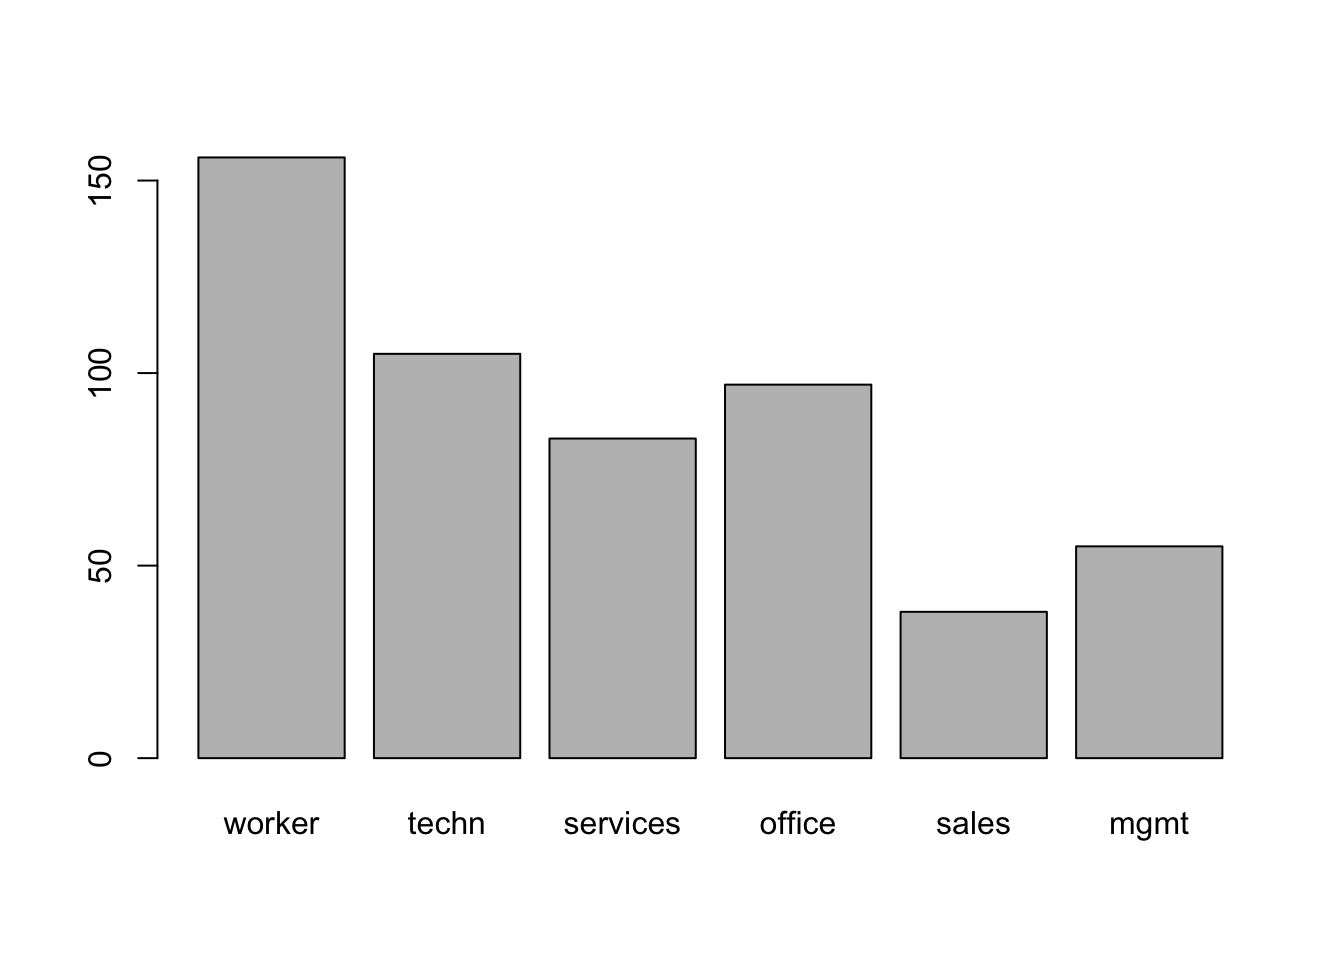
\includegraphics{04-R-Basics-Part4_files/figure-latex/unnamed-chunk-25-1.pdf}

\begin{Shaded}
\begin{Highlighting}[]
\FunctionTok{pie}\NormalTok{(tab, }\AttributeTok{col =} \FunctionTok{gray}\NormalTok{(}\FunctionTok{seq}\NormalTok{(}\FloatTok{0.4}\NormalTok{, }\FloatTok{1.0}\NormalTok{, }\AttributeTok{length =} \DecValTok{6}\NormalTok{)))}
\end{Highlighting}
\end{Shaded}

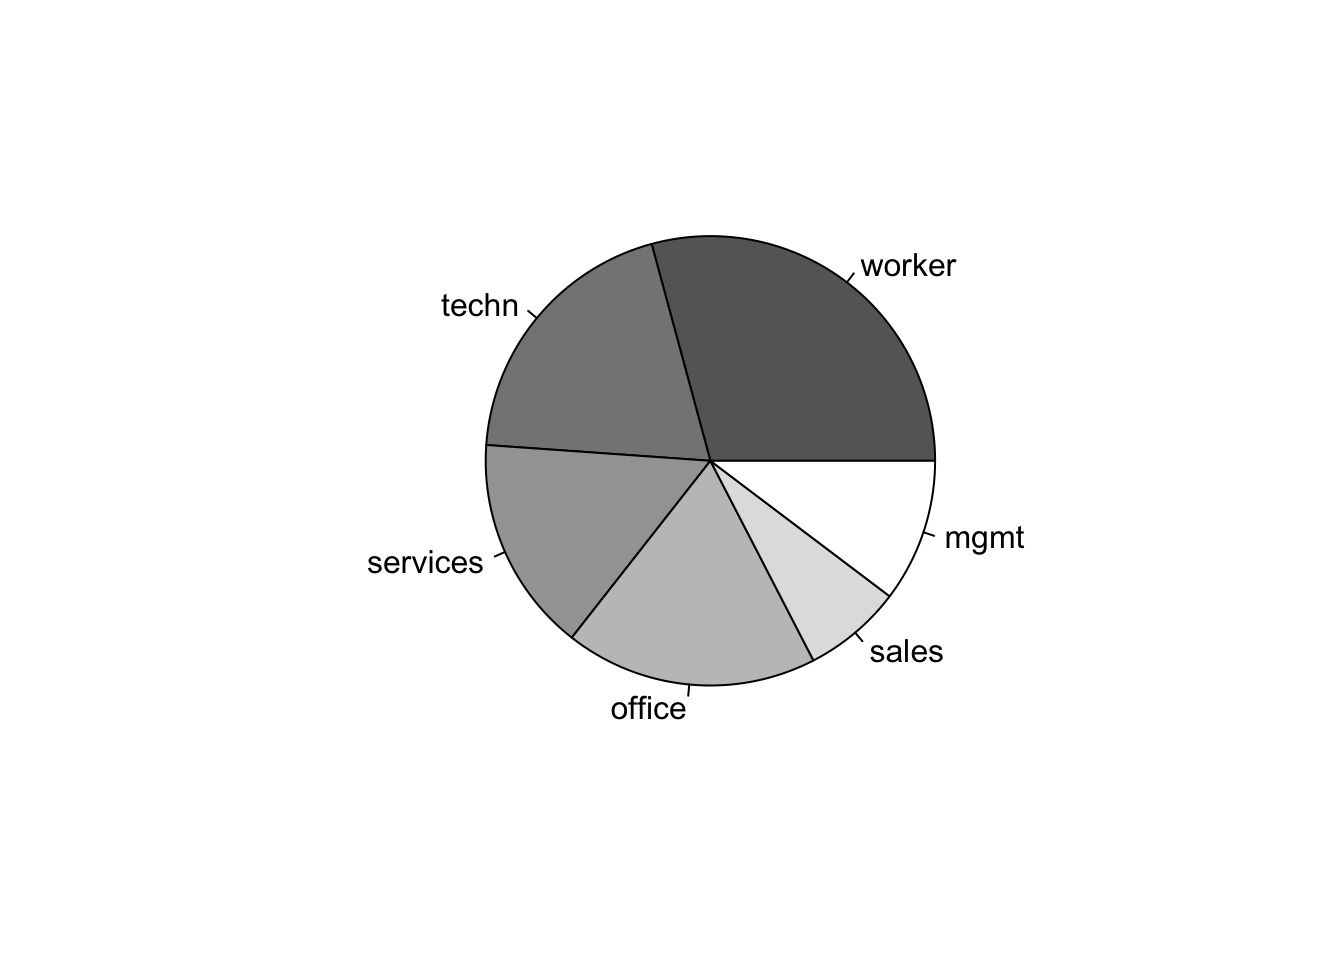
\includegraphics{04-R-Basics-Part4_files/figure-latex/unnamed-chunk-25-2.pdf}

\section*{Two factor variables}\label{two-factor-variables}
\addcontentsline{toc}{section}{Two factor variables}

You now explore the factor variables \texttt{gender} and \texttt{occupation.}

Use \texttt{prop.table()}

The \texttt{prop.table()} function in R is used to compute the proportion of table elements over the margin specified (if any). When applied to a contingency table created by the table() function, it transforms the table's counts into proportions, making it easier to analyze the relative distribution of frequencies across different categories.

\begin{Shaded}
\begin{Highlighting}[]
\FunctionTok{attach}\NormalTok{(CPS1985) }\CommentTok{\# attach the data set to avoid use the operator $}
\FunctionTok{table}\NormalTok{(gender, occupation) }\CommentTok{\# no name\_df$name\_var necessary}
\CommentTok{\#\textgreater{}         occupation}
\CommentTok{\#\textgreater{} gender   worker techn services office sales mgmt}
\CommentTok{\#\textgreater{}   male      126    53       34     21    21   34}
\CommentTok{\#\textgreater{}   female     30    52       49     76    17   21}
\end{Highlighting}
\end{Shaded}

\begin{Shaded}
\begin{Highlighting}[]
\FunctionTok{prop.table}\NormalTok{(}\FunctionTok{table}\NormalTok{(gender, occupation))}
\CommentTok{\#\textgreater{}         occupation}
\CommentTok{\#\textgreater{} gender       worker      techn   services     office}
\CommentTok{\#\textgreater{}   male   0.23595506 0.09925094 0.06367041 0.03932584}
\CommentTok{\#\textgreater{}   female 0.05617978 0.09737828 0.09176030 0.14232210}
\CommentTok{\#\textgreater{}         occupation}
\CommentTok{\#\textgreater{} gender        sales       mgmt}
\CommentTok{\#\textgreater{}   male   0.03932584 0.06367041}
\CommentTok{\#\textgreater{}   female 0.03183521 0.03932584}
\end{Highlighting}
\end{Shaded}

Now try \texttt{prop.table(table(gender,\ occupation),\ 2)}

\begin{Shaded}
\begin{Highlighting}[]
\FunctionTok{prop.table}\NormalTok{(}\FunctionTok{table}\NormalTok{(gender, occupation), }\DecValTok{2}\NormalTok{) }\CommentTok{\# 1 for row , 2 for columns}
\CommentTok{\#\textgreater{}         occupation}
\CommentTok{\#\textgreater{} gender      worker     techn  services    office     sales}
\CommentTok{\#\textgreater{}   male   0.8076923 0.5047619 0.4096386 0.2164948 0.5526316}
\CommentTok{\#\textgreater{}   female 0.1923077 0.4952381 0.5903614 0.7835052 0.4473684}
\CommentTok{\#\textgreater{}         occupation}
\CommentTok{\#\textgreater{} gender        mgmt}
\CommentTok{\#\textgreater{}   male   0.6181818}
\CommentTok{\#\textgreater{}   female 0.3818182}
\end{Highlighting}
\end{Shaded}

You now explore the factor variables gender and occupation.

Do a mosaic plot

A mosaic plot, also known as a Marimekko diagram or a mosaic chart, is a graphical representation of data that allows for the visualization of the proportions or frequencies of categorical variables in a dataset. It's a type of plot that provides a visual summary of the contingency table associated with two or more categorical variables. Each rectangle (tile) in the mosaic plot represents a combination of category levels from the variables, with the area of the rectangle proportional to the frequency or proportion of observations in that category combination.

\begin{Shaded}
\begin{Highlighting}[]
\FunctionTok{plot}\NormalTok{(gender }\SpecialCharTok{\textasciitilde{}}\NormalTok{ occupation, }\AttributeTok{data =}\NormalTok{ CPS1985)}
\end{Highlighting}
\end{Shaded}

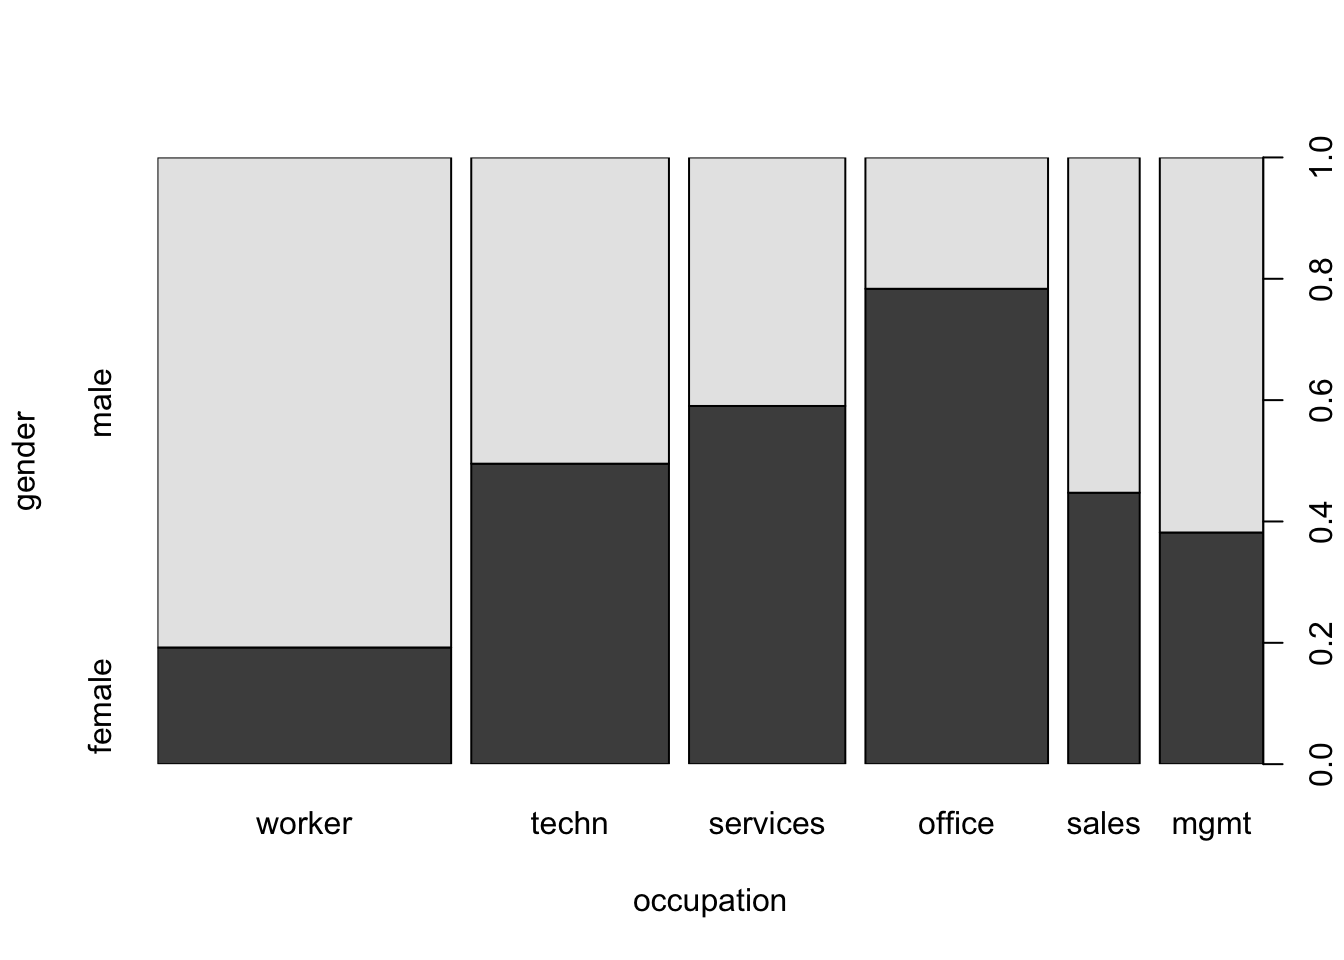
\includegraphics{04-R-Basics-Part4_files/figure-latex/unnamed-chunk-29-1.pdf}

Now explore the factor gender and the numeric variable wage.

The \texttt{tapply()} function in R is used to apply a function to subsets of a vector, where subsets are defined by some other vector, usually a factor. The basic syntax of tapply() is:

\begin{itemize}
\tightlist
\item
  X is the object to be split and operated on.
\item
  INDEX is the factor or list of factors according to which X is split.
\item
  FUN is the function to be applied to each subset of X.
\item
  \ldots{} are optional arguments to FUN.
\item
  simplify, when TRUE, tries to simplify the result to a vector, matrix, or higher-dimensional array; when FALSE, the result is a list.
\end{itemize}

\begin{Shaded}
\begin{Highlighting}[]
\FunctionTok{tapply}\NormalTok{(wage, gender, mean)}
\CommentTok{\#\textgreater{}     male   female }
\CommentTok{\#\textgreater{} 9.994913 7.878857}
\end{Highlighting}
\end{Shaded}

\begin{Shaded}
\begin{Highlighting}[]
\FunctionTok{tapply}\NormalTok{(}\FunctionTok{log}\NormalTok{(wage), }\FunctionTok{list}\NormalTok{(gender, occupation), mean)}
\CommentTok{\#\textgreater{}          worker    techn services   office    sales}
\CommentTok{\#\textgreater{} male   2.100418 2.446640 1.829568 1.955284 2.141071}
\CommentTok{\#\textgreater{} female 1.667887 2.307509 1.701674 1.931128 1.579409}
\CommentTok{\#\textgreater{}            mgmt}
\CommentTok{\#\textgreater{} male   2.447476}
\CommentTok{\#\textgreater{} female 2.229256}
\end{Highlighting}
\end{Shaded}

\section*{A factor and a numeric variable}\label{a-factor-and-a-numeric-variable}
\addcontentsline{toc}{section}{A factor and a numeric variable}

Explore a factor variable and a numeric variable.
Visualize the distribution of \texttt{wage} per \texttt{gender}

\begin{Shaded}
\begin{Highlighting}[]
\FunctionTok{boxplot}\NormalTok{(}\FunctionTok{log}\NormalTok{(wage) }\SpecialCharTok{\textasciitilde{}}\NormalTok{ gender, }\AttributeTok{data =}\NormalTok{ CPS1985)}
\end{Highlighting}
\end{Shaded}

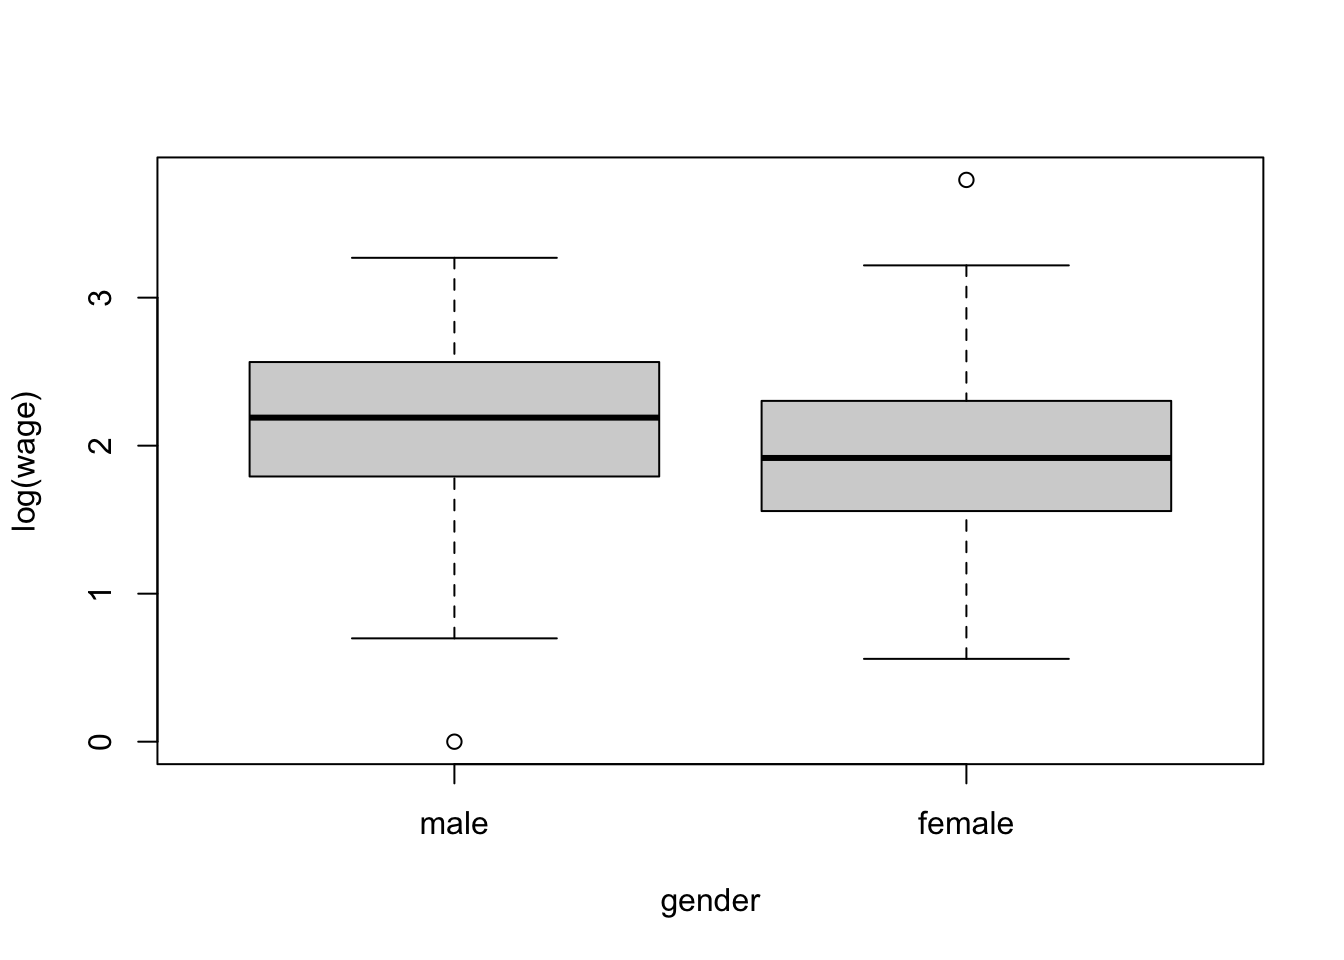
\includegraphics{04-R-Basics-Part4_files/figure-latex/unnamed-chunk-32-1.pdf}

Now try with

\begin{Shaded}
\begin{Highlighting}[]
\FunctionTok{boxplot}\NormalTok{(}\FunctionTok{log}\NormalTok{(wage) }\SpecialCharTok{\textasciitilde{}}\NormalTok{ gender }\SpecialCharTok{+}\NormalTok{ occupation, }\AttributeTok{data =}\NormalTok{ CPS1985)}
\end{Highlighting}
\end{Shaded}

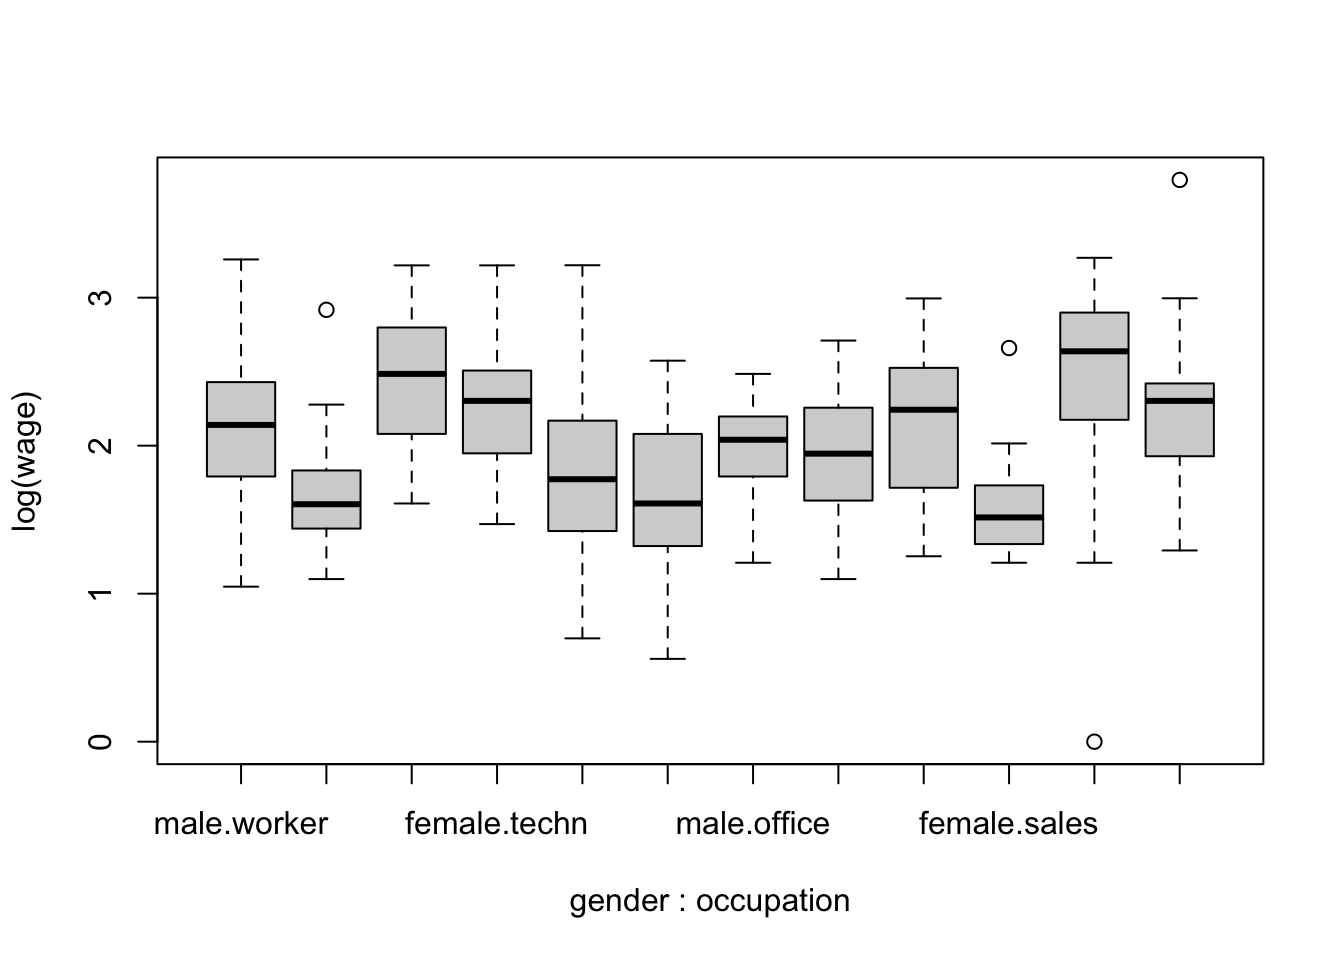
\includegraphics{04-R-Basics-Part4_files/figure-latex/unnamed-chunk-33-1.pdf}

\begin{Shaded}
\begin{Highlighting}[]
\FunctionTok{detach}\NormalTok{(CPS1985) }\CommentTok{\# now detach when work is done}
\end{Highlighting}
\end{Shaded}

\section*{Exercises}\label{exercises}
\addcontentsline{toc}{section}{Exercises}

\begin{enumerate}
\def\labelenumi{\arabic{enumi}.}
\tightlist
\item
  Subsetting Data Frames
\end{enumerate}

Create a data frame named student\_info with the following columns and data:
- student\_id (1 to 5)
- student\_name (`Alice', `Bob', `Charlie', `David', `Eva')
- student\_age (25, 30, 22, 28, 24)
- student\_grade (`A', `B', `A', `C', `B')

Write a command to subset this data frame to include only students older than 24.

\begin{enumerate}
\def\labelenumi{\arabic{enumi}.}
\setcounter{enumi}{1}
\tightlist
\item
  Using Conditional Filters
\end{enumerate}

\begin{itemize}
\tightlist
\item
  Use the subset() function to find all students with a grade of `A'.
\item
  Display the names and ages of these students.
\end{itemize}

\begin{enumerate}
\def\labelenumi{\arabic{enumi}.}
\setcounter{enumi}{2}
\tightlist
\item
  Manipulating Data with dplyr
\end{enumerate}

\begin{itemize}
\item
  Load the dplyr package and convert student\_info to a tibble.
\item
  Use filter() and select() to show the name and age of students who have a grade better than `B'.
\end{itemize}

\begin{enumerate}
\def\labelenumi{\arabic{enumi}.}
\setcounter{enumi}{3}
\tightlist
\item
  Adding and Removing Columns
\end{enumerate}

\begin{itemize}
\tightlist
\item
  Add a new column student\_major with values (`Math', `Science', `Arts', `Math', `Science') to student\_info.
\item
  Then, remove the student\_grade column using dplyr.
\end{itemize}

\begin{enumerate}
\def\labelenumi{\arabic{enumi}.}
\setcounter{enumi}{4}
\tightlist
\item
  Renaming Columns
\end{enumerate}

\begin{itemize}
\tightlist
\item
  Rename the student\_name column to name using base R functions and then using dplyr.
\end{itemize}

\begin{enumerate}
\def\labelenumi{\arabic{enumi}.}
\setcounter{enumi}{5}
\tightlist
\item
  Complex dplyr Operations
\end{enumerate}

\begin{itemize}
\tightlist
\item
  Create a new tibble from student\_info that includes all students except those studying `Arts', rename the student\_id column to id, and arrange the students by age in descending order.
\end{itemize}

\begin{enumerate}
\def\labelenumi{\arabic{enumi}.}
\setcounter{enumi}{6}
\tightlist
\item
  Exploratory Data Analysis with dplyr
\end{enumerate}

\begin{itemize}
\tightlist
\item
  Calculate the average age of students grouped by their major using group\_by() and summarize() in dplyr.
\end{itemize}

\chapter*{Part V: Basic Data Visualization}\label{part-v-basic-data-visualization}
\addcontentsline{toc}{chapter}{Part V: Basic Data Visualization}

\section*{Creating simple plots using plot(), hist(), pie(),barplot(),boxplot()}\label{creating-simple-plots-using-plot-hist-piebarplotboxplot}
\addcontentsline{toc}{section}{Creating simple plots using plot(), hist(), pie(),barplot(),boxplot()}

In R, the \texttt{plot()} function is a generic function used for making a variety of graphs. At its simplest, it is used to create scatter plots but can be customized to create line plots, add model lines, and much more.

\subsection*{Basic Arguments:}\label{basic-arguments}
\addcontentsline{toc}{subsection}{Basic Arguments:}

\begin{itemize}
\tightlist
\item
  \texttt{x}: The coordinates of points in the plot. For a simple scatter plot, this is typically a numeric vector.
\item
  \texttt{y}: The coordinates of points in the plot on the y-axis. Should be the same length as x.
\item
  \texttt{type}: What type of plot should be drawn. Possible types include ``p'' for points (the default), ``l'' for lines, ``b'' for both, and several others.
\item
  \texttt{main}: The main title of the plot.
\item
  \texttt{xlab}: The label for the x-axis.
\item
  \texttt{ylab}: The label for the y-axis.
\item
  \texttt{xlim}: Limits for the x-axis.
\item
  \texttt{ylim}: Limits for the y-axis.
\item
  \texttt{pch}: Plotting character, or symbol to use in the plot. Different numbers correspond to different symbols.
\item
  \texttt{col}: Color for the points. Can also be a vector to color points differently based on a factor.
\end{itemize}

\subsection*{Additional Customizations:}\label{additional-customizations}
\addcontentsline{toc}{subsection}{Additional Customizations:}

\begin{itemize}
\tightlist
\item
  \texttt{cex}: A numerical value giving the amount by which plotting text and symbols should be magnified relative to the default.
\item
  \texttt{lwd}: Line width for the plot, useful when the plot type includes lines.
\item
  \texttt{bg}: Background color for the open plot symbols specified by pch.
  Advanced Features:
\item
  \texttt{abline}: A function to add straight lines to a plot, either vertical, horizontal, or regression lines.
\item
  \texttt{lines}: A function to add lines to a plot, in the context of the existing plot; it doesn't start a new plot.
  points: Add points to a plot.
\end{itemize}

\subsection*{Adding a Legend:}\label{adding-a-legend}
\addcontentsline{toc}{subsection}{Adding a Legend:}

To add a legend, you use the \texttt{legend()} function. It provides a number of arguments to customize its appearance:

\texttt{legend}: A vector of text values or an expression describing the text to appear in the legend.
\texttt{x,\ y} or \texttt{position}: The location of the legend. \texttt{x} and \texttt{y} can be numeric positions, or you can use keyword positions like \texttt{"topright"}, \texttt{"bottomleft"}, \texttt{"bottomright"} , \texttt{"bottom"}, \texttt{"bottomleft"}, \texttt{"left"}, \texttt{"topleft"}, \texttt{"top"}, \texttt{"right"}, \texttt{"center"}.
\texttt{pch}: The plotting symbols for points appearing in the legend, matching those in the plot.
\texttt{col}: The colors for points or lines appearing in the legend, matching those in the plot.
\texttt{lwd}: The line widths for lines appearing in the legend, matching those in the plot.
\texttt{cex}: Character expansion size for the legend, determining how large the text in the legend should be.

\section*{Example 1 : Simple scatter plot}\label{example-1-simple-scatter-plot}
\addcontentsline{toc}{section}{Example 1 : Simple scatter plot}

\begin{Shaded}
\begin{Highlighting}[]

\NormalTok{x }\OtherTok{\textless{}{-}} \DecValTok{1}\SpecialCharTok{:}\DecValTok{10}
\NormalTok{y }\OtherTok{\textless{}{-}} \FunctionTok{rnorm}\NormalTok{(}\DecValTok{10}\NormalTok{)}
\FunctionTok{plot}\NormalTok{(x, y, }\AttributeTok{main =} \StringTok{"Simple Scatter Plot"}\NormalTok{, }\AttributeTok{xlab =} \StringTok{"X Axis"}\NormalTok{, }\AttributeTok{ylab =} \StringTok{"Y Axis"}\NormalTok{, }\AttributeTok{col =} \StringTok{"blue"}\NormalTok{)}
\end{Highlighting}
\end{Shaded}

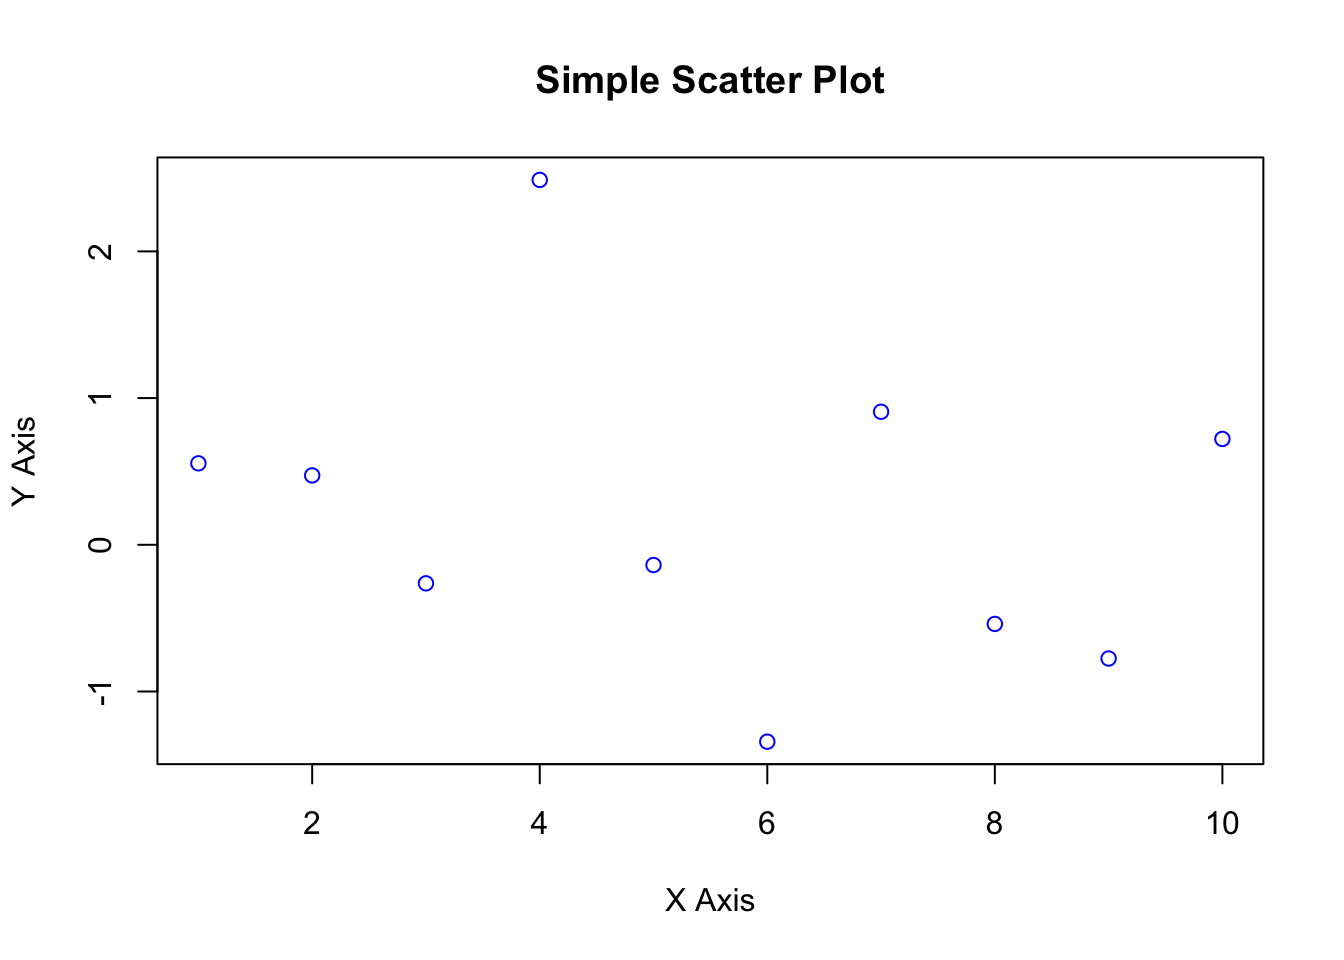
\includegraphics{05-R-Basic-Part5_files/figure-latex/unnamed-chunk-1-1.pdf}

\section*{Exercise 1}\label{exercise-1-2}
\addcontentsline{toc}{section}{Exercise 1}

Making a Scatter plot:

\begin{itemize}
\tightlist
\item
  load the journals.txt data set and save as Journals data frame
\item
  Work through the following instructions
\end{itemize}

\begin{Shaded}
\begin{Highlighting}[]
\FunctionTok{plot}\NormalTok{(}\FunctionTok{log}\NormalTok{(Journals}\SpecialCharTok{$}\NormalTok{subs), }\FunctionTok{log}\NormalTok{(Journals}\SpecialCharTok{$}\NormalTok{price))}
\FunctionTok{rug}\NormalTok{(}\FunctionTok{log}\NormalTok{(Journals}\SpecialCharTok{$}\NormalTok{subs))}
\FunctionTok{rug}\NormalTok{(}\FunctionTok{log}\NormalTok{(Journals}\SpecialCharTok{$}\NormalTok{price), }\AttributeTok{side =} \DecValTok{2}\NormalTok{)}
\end{Highlighting}
\end{Shaded}

Now adjust the plotting instructions

\begin{Shaded}
\begin{Highlighting}[]
\FunctionTok{plot}\NormalTok{(}\FunctionTok{log}\NormalTok{(Journals}\SpecialCharTok{$}\NormalTok{price) }\SpecialCharTok{\textasciitilde{}} \FunctionTok{log}\NormalTok{(Journals}\SpecialCharTok{$}\NormalTok{subs), }\AttributeTok{pch =} \DecValTok{19}\NormalTok{,}
     \AttributeTok{col =} \StringTok{"blue"}\NormalTok{, }\AttributeTok{xlim =} \FunctionTok{c}\NormalTok{(}\DecValTok{0}\NormalTok{, }\DecValTok{7}\NormalTok{), }\AttributeTok{ylim =} \FunctionTok{c}\NormalTok{(}\DecValTok{3}\NormalTok{, }\DecValTok{8}\NormalTok{),}
     \AttributeTok{main =} \StringTok{"Library subscriptions"}\NormalTok{)}
\FunctionTok{rug}\NormalTok{(}\FunctionTok{log}\NormalTok{(Journals}\SpecialCharTok{$}\NormalTok{subs))}
\FunctionTok{rug}\NormalTok{(}\FunctionTok{log}\NormalTok{(Journals}\SpecialCharTok{$}\NormalTok{price), }\AttributeTok{side=}\DecValTok{2}\NormalTok{)}
\end{Highlighting}
\end{Shaded}

The \texttt{curve()} function draws a curve corresponding to a function over the interval {[}from, to{]}.

\begin{Shaded}
\begin{Highlighting}[]
\FunctionTok{curve}\NormalTok{(dnorm, }\AttributeTok{from =} \SpecialCharTok{{-}}\DecValTok{5}\NormalTok{, }\AttributeTok{to =} \DecValTok{5}\NormalTok{, }\AttributeTok{col =} \StringTok{"red"}\NormalTok{, }\AttributeTok{lwd =} \DecValTok{3}\NormalTok{,}
      \AttributeTok{main =} \StringTok{"Density of the standard normal distribution"}\NormalTok{)}
\end{Highlighting}
\end{Shaded}

\includegraphics{05-R-Basic-Part5_files/figure-latex/unnamed-chunk-4-1.pdf}

\section*{Example 2}\label{example-2}
\addcontentsline{toc}{section}{Example 2}

To create a basic scatter plot, you can use the mtcars dataset, which comes built into R. This dataset contains various characteristics of 32 automobiles.

\begin{Shaded}
\begin{Highlighting}[]

\FunctionTok{data}\NormalTok{(mtcars)}


\FunctionTok{plot}\NormalTok{(mtcars}\SpecialCharTok{$}\NormalTok{hp, mtcars}\SpecialCharTok{$}\NormalTok{mpg, }\AttributeTok{main=}\StringTok{"MPG vs. Horsepower"}\NormalTok{,}
     \AttributeTok{xlab=}\StringTok{"Horsepower"}\NormalTok{, }\AttributeTok{ylab=}\StringTok{"Miles Per Gallon"}\NormalTok{,}
     \AttributeTok{pch=}\DecValTok{19}\NormalTok{, }\AttributeTok{col=}\StringTok{"blue"}\NormalTok{)}
\end{Highlighting}
\end{Shaded}

\includegraphics{05-R-Basic-Part5_files/figure-latex/unnamed-chunk-5-1.pdf}

\section*{Example 3}\label{example-3}
\addcontentsline{toc}{section}{Example 3}

Using the pressure dataset, which is also built into R, you can create a simple line plot. The pressure dataset shows the temperature and resulting vapor pressure of mercury.

\begin{Shaded}
\begin{Highlighting}[]

\FunctionTok{data}\NormalTok{(pressure)}

\CommentTok{\# Create a line plot}
\FunctionTok{plot}\NormalTok{(pressure}\SpecialCharTok{$}\NormalTok{temperature, pressure}\SpecialCharTok{$}\NormalTok{pressure, }\AttributeTok{type=}\StringTok{"l"}\NormalTok{,}
     \AttributeTok{main=}\StringTok{"Vapor Pressure of Mercury"}\NormalTok{,}
     \AttributeTok{xlab=}\StringTok{"Temperature"}\NormalTok{, }\AttributeTok{ylab=}\StringTok{"Pressure"}\NormalTok{,}
     \AttributeTok{col=}\StringTok{"red"}\NormalTok{, }\AttributeTok{lwd=}\DecValTok{2}\NormalTok{)}
\end{Highlighting}
\end{Shaded}

\includegraphics{05-R-Basic-Part5_files/figure-latex/unnamed-chunk-6-1.pdf}

\section*{Example 4}\label{example-4}
\addcontentsline{toc}{section}{Example 4}

\begin{Shaded}
\begin{Highlighting}[]
\CommentTok{\# Load the mtcars dataset}
\FunctionTok{data}\NormalTok{(mtcars)}

\CommentTok{\# Plot MPG vs. Displacement, colored by Cylinders}
\FunctionTok{plot}\NormalTok{(mtcars}\SpecialCharTok{$}\NormalTok{disp, mtcars}\SpecialCharTok{$}\NormalTok{mpg, }\AttributeTok{col=}\FunctionTok{as.factor}\NormalTok{(mtcars}\SpecialCharTok{$}\NormalTok{cyl),}
     \AttributeTok{main=}\StringTok{"Scatter Plot of MPG vs. Displacement"}\NormalTok{,}
     \AttributeTok{xlab=}\StringTok{"Displacement (cu.in.)"}\NormalTok{, }\AttributeTok{ylab=}\StringTok{"MPG"}\NormalTok{,}
     \AttributeTok{pch=}\DecValTok{19}\NormalTok{, }\AttributeTok{cex=}\FloatTok{1.5}\NormalTok{)}

\CommentTok{\# Add a legend to the plot}
\FunctionTok{legend}\NormalTok{(}\StringTok{"topright"}\NormalTok{, }
       \AttributeTok{legend=}\FunctionTok{paste}\NormalTok{(}\StringTok{"Cylinders:"}\NormalTok{, }\FunctionTok{unique}\NormalTok{(mtcars}\SpecialCharTok{$}\NormalTok{cyl)), }
       \AttributeTok{col=}\FunctionTok{unique}\NormalTok{(}\FunctionTok{as.numeric}\NormalTok{(}\FunctionTok{as.factor}\NormalTok{(mtcars}\SpecialCharTok{$}\NormalTok{cyl))), }
       \AttributeTok{pch=}\DecValTok{19}\NormalTok{, }\AttributeTok{cex=}\FloatTok{0.8}\NormalTok{)}
\end{Highlighting}
\end{Shaded}

\includegraphics{05-R-Basic-Part5_files/figure-latex/unnamed-chunk-7-1.pdf}

\begin{itemize}
\tightlist
\item
  \texttt{plot()} is the generic function to create a scatter plot.
  mtcars\(disp and mtcars\)mpg are the x and y coordinates for the plot, representing the engine displacement in cubic inches and miles per gallon, respectively.
\item
  \texttt{col=as.factor(mtcars\$cyl)} specifies the colors for the points on the plot. The cyl variable, which represents the number of cylinders in the car's engine, is converted into a factor. The levels of this factor (unique values of cyl) are automatically given different colors.
\item
  \texttt{main} is the main title for the plot.
\item
  \texttt{xlab} and \texttt{ylab} are labels for the x-axis and y-axis, respectively.
\item
  \texttt{pch=19} specifies the plotting symbol (in this case, a solid circle).
\item
  \texttt{cex=1.5} sets the size of the plot symbols; cex stands for character expansion factor, where 1.5 means 150\% of the default size.
\end{itemize}

For the legend,

\begin{itemize}
\tightlist
\item
  \texttt{legend()} adds a legend to the plot.
\item
  \texttt{"topright"} specifies the position of the legend (in this case, at the top right corner of the plotting area).
\item
  \texttt{legend}= creates the text for the legend by pasting the word ``Cylinders:'' in front of each unique value of the cyl column. This indicates what each color in the scatter plot corresponds to.
\item
  \texttt{col=} sets the colors used in the legend, which match the colors used for the points in the plot.
\item
  \texttt{pch=19} again specifies the plotting symbols used in the legend.
\item
  \texttt{cex=0.8} sets the size of the symbols in the legend.
\end{itemize}

\section*{Example 5}\label{example-5}
\addcontentsline{toc}{section}{Example 5}

\subsection*{Scatterplot()}\label{scatterplot}
\addcontentsline{toc}{subsection}{Scatterplot()}

The most common high level function used to produce plots in \texttt{R} is (rather unsurprisingly) the \texttt{plot()} function. For example, let's plot the weight of petunia plants from our flowers data frame from \texttt{flower.xls}

Use the library \texttt{readxl}, and \texttt{read\_excel()} function.

Alternatively , you can also use \texttt{flower.txt} and use read\_table

\begin{Shaded}
\begin{Highlighting}[]

\FunctionTok{library}\NormalTok{(readxl)}
\NormalTok{flowers }\OtherTok{\textless{}{-}} \FunctionTok{read\_excel}\NormalTok{(}\StringTok{\textquotesingle{}./Data/flower.xls\textquotesingle{}}\NormalTok{)}

\FunctionTok{plot}\NormalTok{(flowers}\SpecialCharTok{$}\NormalTok{weight)}
\end{Highlighting}
\end{Shaded}

\includegraphics{05-R-Basic-Part5_files/figure-latex/unnamed-chunk-8-1.pdf}

\begin{Shaded}
\begin{Highlighting}[]
\NormalTok{flowers }\OtherTok{\textless{}{-}} \FunctionTok{read.table}\NormalTok{(}\AttributeTok{file =} \StringTok{\textquotesingle{}./Data/flower.txt\textquotesingle{}}\NormalTok{, }
                        \AttributeTok{header =} \ConstantTok{TRUE}\NormalTok{, }\AttributeTok{sep =} \StringTok{"}\SpecialCharTok{\textbackslash{}t}\StringTok{"}\NormalTok{, }
                        \AttributeTok{stringsAsFactors =} \ConstantTok{TRUE}\NormalTok{)}
\end{Highlighting}
\end{Shaded}

To plot a scatterplot of one numeric variable against another numeric variable we just need to include both variables as arguments when using the \texttt{plot()} function. For example to plot \texttt{shootarea} on the y axis and \texttt{weight} of the x axis.

\begin{Shaded}
\begin{Highlighting}[]
\FunctionTok{plot}\NormalTok{(}\AttributeTok{x =}\NormalTok{ flowers}\SpecialCharTok{$}\NormalTok{weight, }\AttributeTok{y =}\NormalTok{ flowers}\SpecialCharTok{$}\NormalTok{shootarea)}
\end{Highlighting}
\end{Shaded}

\includegraphics{05-R-Basic-Part5_files/figure-latex/unnamed-chunk-10-1.pdf}

There is an equivalent approach for these types of plots which often causes some confusion at first. You can also use the formula notation when using the \texttt{plot()} function. However, in contrast to the previous method the formula method requires you to specify the y axis variable first, then a \texttt{\textasciitilde{}}and then our x axis variable.

\begin{Shaded}
\begin{Highlighting}[]
\FunctionTok{plot}\NormalTok{(flowers}\SpecialCharTok{$}\NormalTok{shootarea }\SpecialCharTok{\textasciitilde{}}\NormalTok{ flowers}\SpecialCharTok{$}\NormalTok{weight)}
\end{Highlighting}
\end{Shaded}

\includegraphics{05-R-Basic-Part5_files/figure-latex/unnamed-chunk-11-1.pdf}

\subsection*{Histogram}\label{histogram}
\addcontentsline{toc}{subsection}{Histogram}

\begin{Shaded}
\begin{Highlighting}[]
\FunctionTok{hist}\NormalTok{(flowers}\SpecialCharTok{$}\NormalTok{height)}
\end{Highlighting}
\end{Shaded}

\includegraphics{05-R-Basic-Part5_files/figure-latex/unnamed-chunk-12-1.pdf}

\begin{Shaded}
\begin{Highlighting}[]
\NormalTok{brk }\OtherTok{\textless{}{-}} \FunctionTok{seq}\NormalTok{(}\AttributeTok{from =} \DecValTok{0}\NormalTok{, }\AttributeTok{to =} \DecValTok{18}\NormalTok{, }\AttributeTok{by =} \DecValTok{1}\NormalTok{)}
\FunctionTok{hist}\NormalTok{(flowers}\SpecialCharTok{$}\NormalTok{height, }\AttributeTok{breaks =}\NormalTok{ brk, }\AttributeTok{main =} \StringTok{"petunia height"}\NormalTok{)}
\end{Highlighting}
\end{Shaded}

\includegraphics{05-R-Basic-Part5_files/figure-latex/unnamed-chunk-13-1.pdf}

You can also display the histogram as a proportion rather than a frequency by using the freq = FALSE argument.

\begin{Shaded}
\begin{Highlighting}[]
\NormalTok{brk }\OtherTok{\textless{}{-}} \FunctionTok{seq}\NormalTok{(}\AttributeTok{from =} \DecValTok{0}\NormalTok{, }\AttributeTok{to =} \DecValTok{18}\NormalTok{, }\AttributeTok{by =} \DecValTok{1}\NormalTok{)}
\FunctionTok{hist}\NormalTok{(flowers}\SpecialCharTok{$}\NormalTok{height, }\AttributeTok{breaks =}\NormalTok{ brk, }\AttributeTok{main =} \StringTok{"petunia height"}\NormalTok{,}
      \AttributeTok{freq =} \ConstantTok{FALSE}\NormalTok{)}
\end{Highlighting}
\end{Shaded}

\includegraphics{05-R-Basic-Part5_files/figure-latex/unnamed-chunk-14-1.pdf}

An alternative to plotting just a straight up histogram is to add a kernel density curve to the plot. You can superimpose a density curve onto the histogram by first using the density() function to compute the kernel density estimates and then use the low level function lines() to add these estimates onto the plot as a line.

\begin{Shaded}
\begin{Highlighting}[]
\NormalTok{dens }\OtherTok{\textless{}{-}} \FunctionTok{density}\NormalTok{(flowers}\SpecialCharTok{$}\NormalTok{height)}
\FunctionTok{hist}\NormalTok{(flowers}\SpecialCharTok{$}\NormalTok{height, }\AttributeTok{breaks =}\NormalTok{ brk, }\AttributeTok{main =} \StringTok{"petunia height"}\NormalTok{,}
      \AttributeTok{freq =} \ConstantTok{FALSE}\NormalTok{)}
\FunctionTok{lines}\NormalTok{(dens)}
\end{Highlighting}
\end{Shaded}

\includegraphics{05-R-Basic-Part5_files/figure-latex/unnamed-chunk-15-1.pdf}

\section*{Boxplot}\label{boxplot}
\addcontentsline{toc}{section}{Boxplot}

OK, we'll just come and out and say it, we love boxplots and their close relation the violin plot. Boxplots (or box-and-whisker plots to give them their full name) are very useful when you want to graphically summarise the distribution of a variable, identify potential unusual values and compare distributions between different groups. The reason we love them is their ease of interpretation, transparency and relatively high data-to-ink ratio (i.e.~they convey lots of information efficiently). We suggest that you try to use boxplots as much as possible when exploring your data and avoid the temptation to use the more ubiquitous bar plot (even with standard error or 95\% confidence intervals bars). The problem with bar plots (aka dynamite plots) is that they hide important information from the reader such as the distribution of the data and assume that the error bars (or confidence intervals) are symmetric around the mean. Of course, it's up to you what you do but if you're tempted to use bar plots just Google `dynamite plots are evil' \href{http://users.stat.umn.edu/~rend0020/Teaching/STAT8801-2015Spring/handouts/24-dynamite.pdf}{see here} or \href{https://thenode.biologists.com/leaving-bar-five-steps/research/}{here}

To create a boxplot in R we use the boxplot() function. For example, let's create a boxplot of the variable weight from our flowers data frame. We can also include a y axis label using the ylab = argument.

\begin{Shaded}
\begin{Highlighting}[]
\FunctionTok{boxplot}\NormalTok{(flowers}\SpecialCharTok{$}\NormalTok{weight, }\AttributeTok{ylab =} \StringTok{"weight (g)"}\NormalTok{)}
\end{Highlighting}
\end{Shaded}

\includegraphics{05-R-Basic-Part5_files/figure-latex/unnamed-chunk-16-1.pdf}
The thick horizontal line in the middle of the box is the median value of weight (around 11 g). The upper line of the box is the upper quartile (75th percentile) and the lower line is the lower quartile (25th percentile). The distance between the upper and lower quartiles is known as the inter quartile range and represents the values of weight for 50\% of the data. The dotted vertical lines are called the whiskers and their length is determined as 1.5 x the inter quartile range. Data points that are plotted outside the the whiskers represent potential unusual observations. This doesn't mean they are unusual, just that they warrant a closer look. We recommend using boxplots in combination with Cleveland dotplots to identify potential unusual observations (see the next section of this Chapter for more details). The neat thing about boxplots is that they not only provide a measure of central tendency (the median value) they also give you an idea about the distribution of the data. If the median line is more or less in the middle of the box (between the upper and lower quartiles) and the whiskers are more or less the same length then you can be reasonably sure the distribution of your data is symmetrical.

If we want examine how the distribution of a variable changes between different levels of a factor we need to use the formula notation with the boxplot() function. For example, let's plot our weight variable again, but this time see how this changes with each level of nitrogen. When we use the formula notation with \texttt{boxplot()} we can use the data = argument to save some typing. We'll also introduce an x axis label using the xlab = argument.

\begin{Shaded}
\begin{Highlighting}[]
\FunctionTok{boxplot}\NormalTok{(weight }\SpecialCharTok{\textasciitilde{}}\NormalTok{ nitrogen, }\AttributeTok{data =}\NormalTok{ flowers, }
         \AttributeTok{ylab =} \StringTok{"weight (g)"}\NormalTok{, }\AttributeTok{xlab =} \StringTok{"nitrogen level"}\NormalTok{)}
\end{Highlighting}
\end{Shaded}

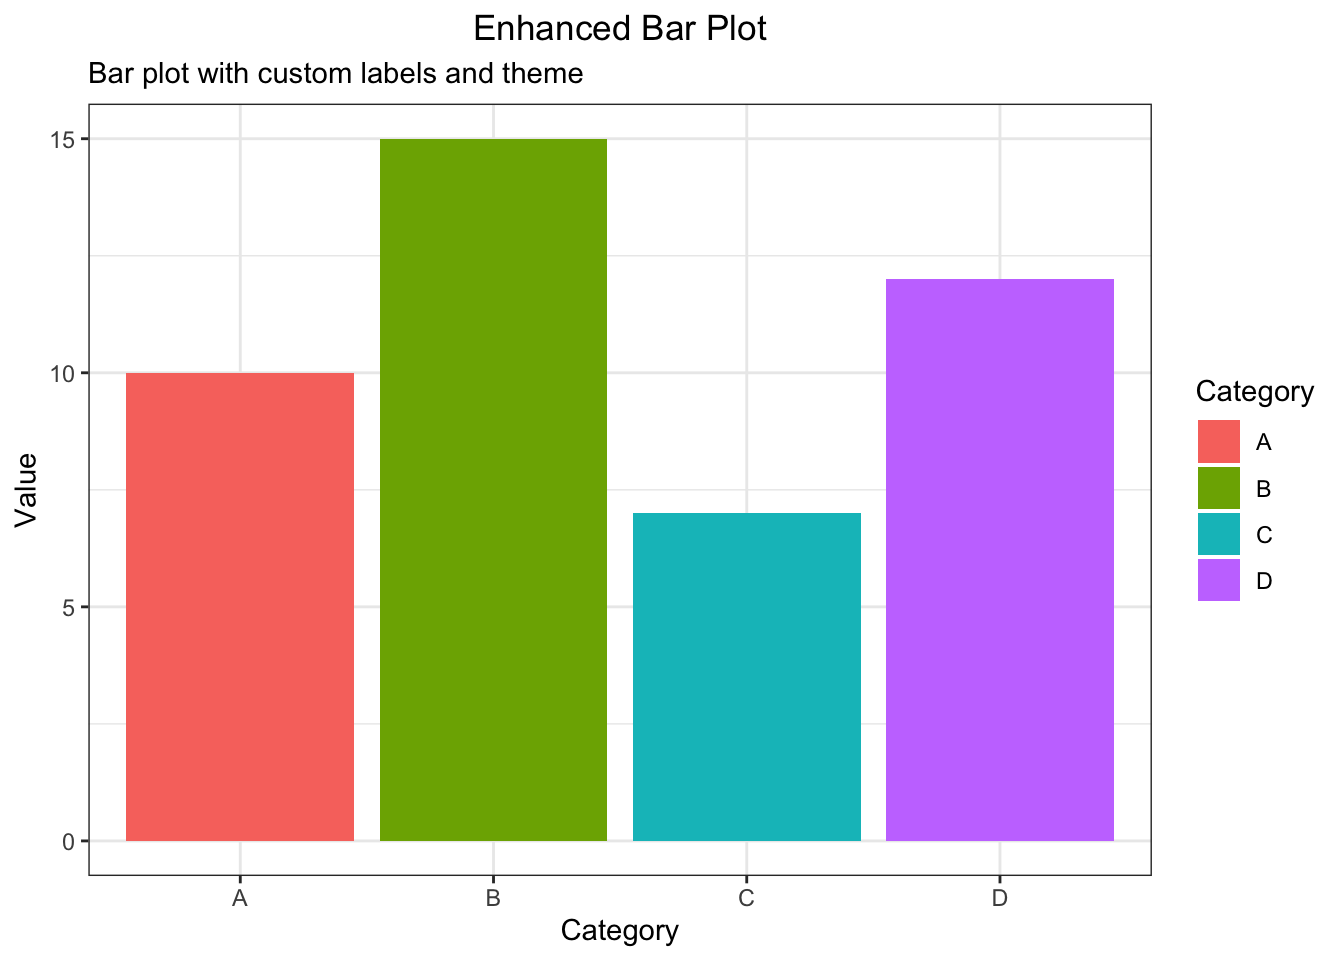
\includegraphics{05-R-Basic-Part5_files/figure-latex/unnamed-chunk-17-1.pdf}

The factor levels are plotted in the same order defined by our factor variable nitrogen (often alphabetically). To change the order we need to change the order of our levels of the nitrogen factor in our data frame using the factor() function and then re-plot the graph. Let's plot our boxplot with our factor levels going from low to high.

\begin{Shaded}
\begin{Highlighting}[]
\NormalTok{flowers}\SpecialCharTok{$}\NormalTok{nitrogen }\OtherTok{\textless{}{-}} \FunctionTok{factor}\NormalTok{(flowers}\SpecialCharTok{$}\NormalTok{nitrogen, }
                            \AttributeTok{levels =} \FunctionTok{c}\NormalTok{(}\StringTok{"low"}\NormalTok{, }\StringTok{"medium"}\NormalTok{, }\StringTok{"high"}\NormalTok{))}
\FunctionTok{boxplot}\NormalTok{(weight }\SpecialCharTok{\textasciitilde{}}\NormalTok{ nitrogen, }\AttributeTok{data =}\NormalTok{ flowers, }
          \AttributeTok{ylab =} \StringTok{"weight (g)"}\NormalTok{, }\AttributeTok{xlab =} \StringTok{"nitrogen level"}\NormalTok{)}
\end{Highlighting}
\end{Shaded}

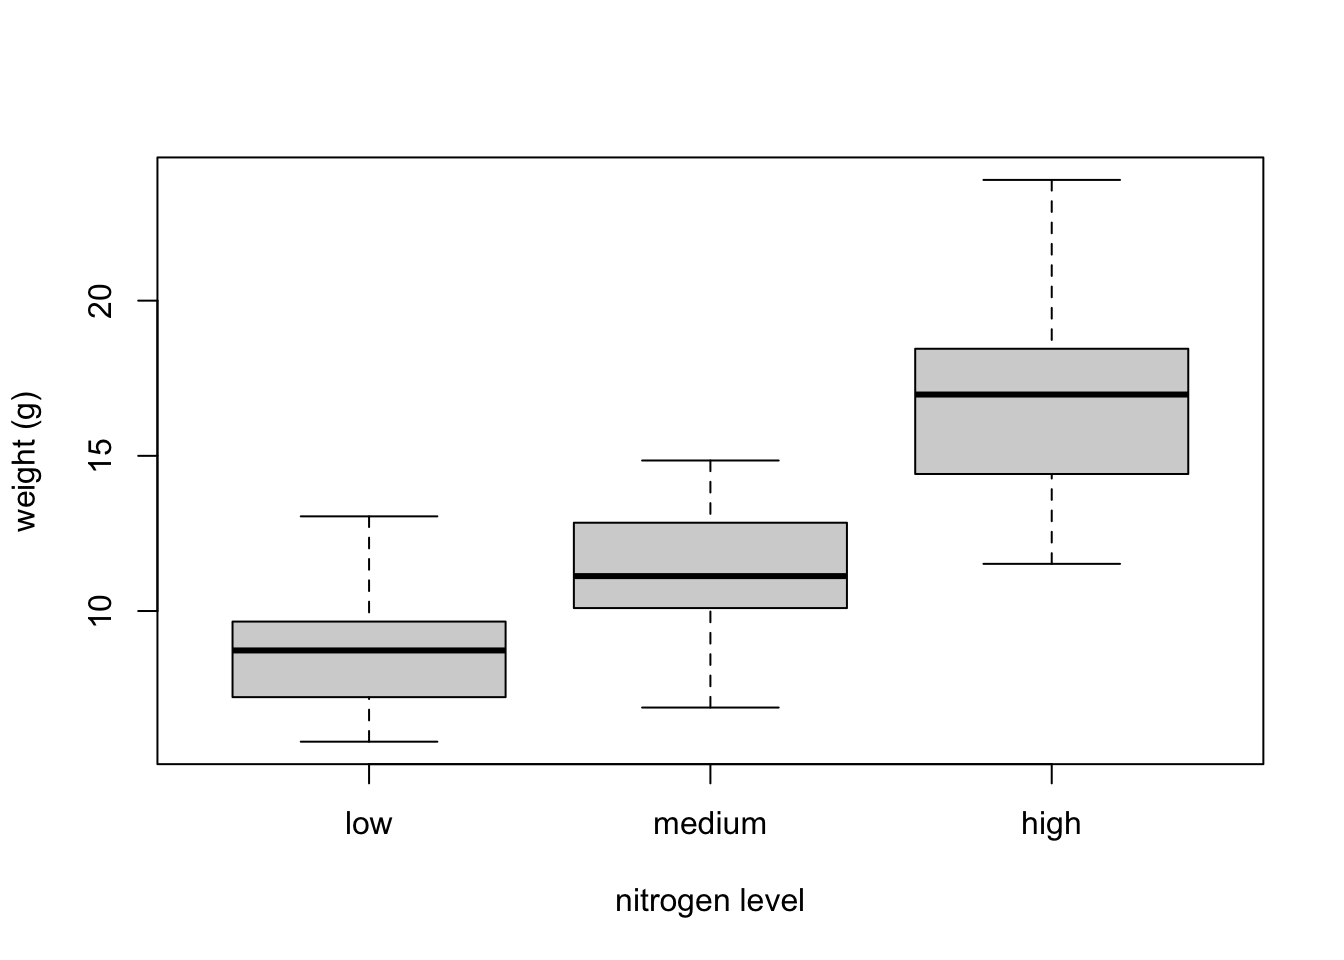
\includegraphics{05-R-Basic-Part5_files/figure-latex/unnamed-chunk-18-1.pdf}

We can also group our variables by two factors in the same plot. Let's plot our weight variable but this time plot a separate box for each nitrogen and treatment (treat) combination.

\begin{Shaded}
\begin{Highlighting}[]
\FunctionTok{boxplot}\NormalTok{(weight }\SpecialCharTok{\textasciitilde{}}\NormalTok{ nitrogen }\SpecialCharTok{*}\NormalTok{ treat, }\AttributeTok{data =}\NormalTok{ flowers, }
         \AttributeTok{ylab =} \StringTok{"weight (g)"}\NormalTok{, }\AttributeTok{xlab =} \StringTok{"nitrogen level"}\NormalTok{)}
\end{Highlighting}
\end{Shaded}

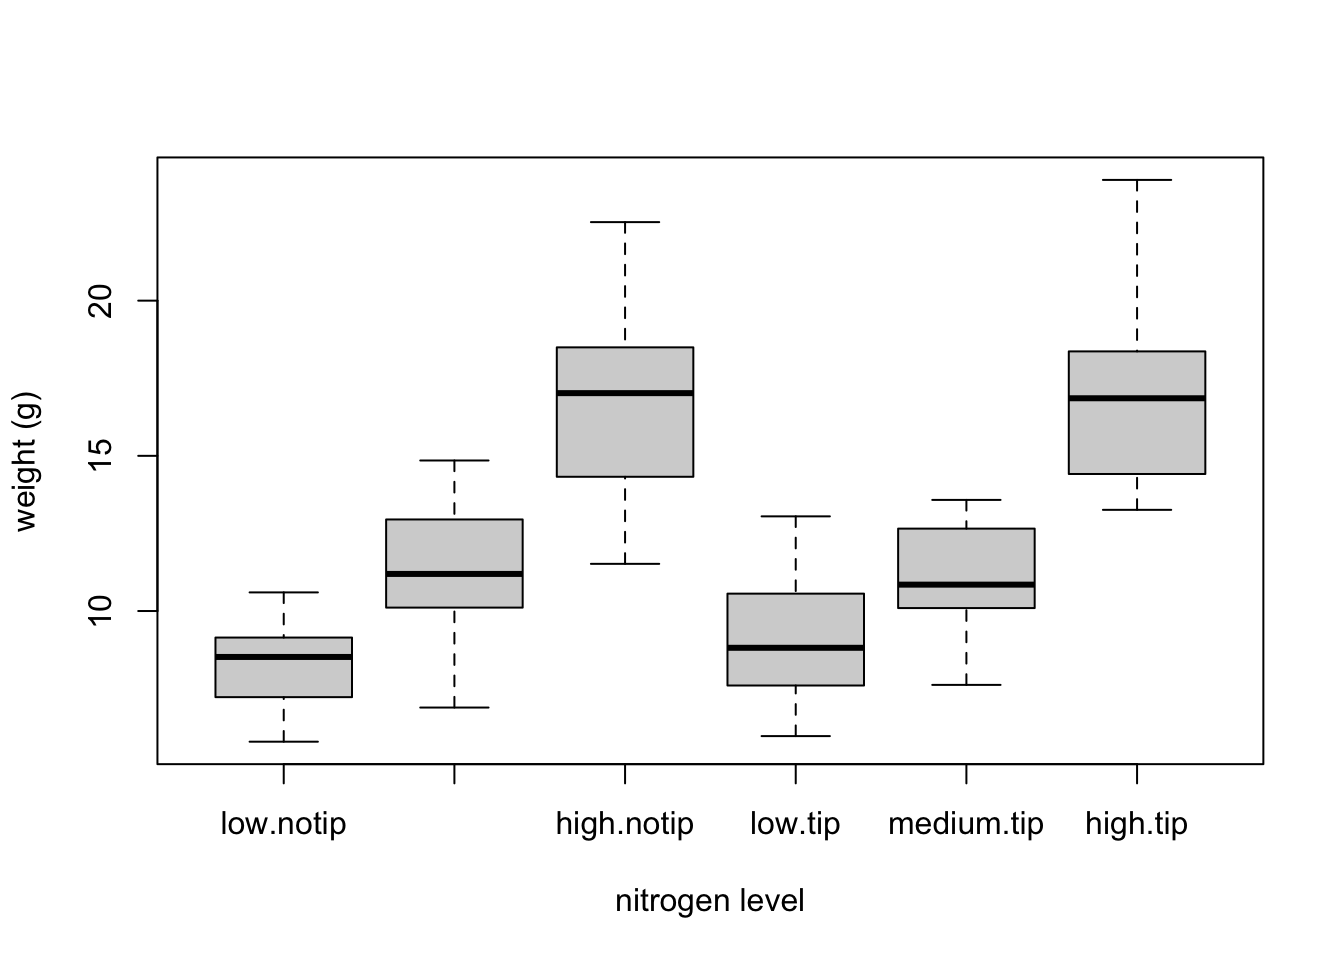
\includegraphics{05-R-Basic-Part5_files/figure-latex/unnamed-chunk-19-1.pdf}

This plot looks OK, but some of the group labels are hidden as they're too long to fit on the plot. There are a couple of ways to deal with this. Perhaps the easiest is to reduce the font size of the tick mark labels in the plot so they all fit using the \texttt{cex.axis\ =} argument. Let's set the font size to be 30\% smaller than the default with \texttt{cex.axis\ =\ 0.7}

\begin{Shaded}
\begin{Highlighting}[]
\FunctionTok{boxplot}\NormalTok{(weight }\SpecialCharTok{\textasciitilde{}}\NormalTok{ nitrogen }\SpecialCharTok{*}\NormalTok{ treat, }\AttributeTok{data =}\NormalTok{ flowers, }
         \AttributeTok{ylab =} \StringTok{"weight (g)"}\NormalTok{, }\AttributeTok{xlab =} \StringTok{"nitrogen level"}\NormalTok{, }
         \AttributeTok{cex.axis =} \FloatTok{0.7}\NormalTok{)}
\end{Highlighting}
\end{Shaded}

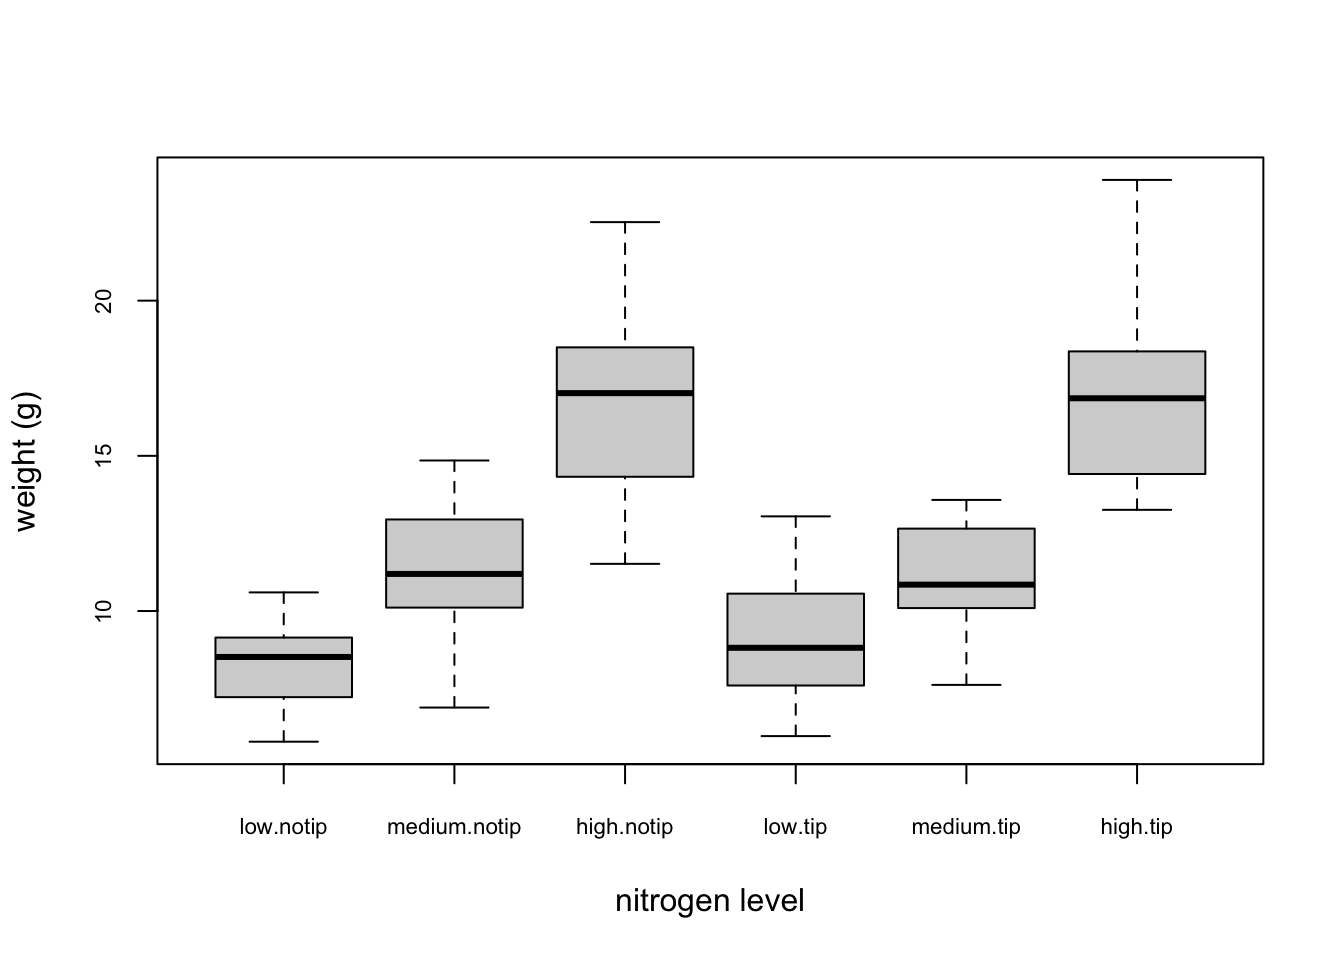
\includegraphics{05-R-Basic-Part5_files/figure-latex/unnamed-chunk-20-1.pdf}
\#\# Violin Plots \{-\}

Violin plots are like a combination of a boxplot and a kernel density plot (you saw an example of a kernel density plot in the histogram section above) all rolled into one figure. We can create a violin plot in R using the vioplot() function from the vioplot package. You'll need to first install this package using install.packages(`vioplot') function as usual. The nice thing about the vioplot() function is that you use it in pretty much the same way you would use the boxplot() function. We'll also use the argument col = ``lightblue'' to change the fill colour to light blue.

\begin{Shaded}
\begin{Highlighting}[]
\CommentTok{\#install.packages("vioplot")}
\FunctionTok{library}\NormalTok{(vioplot)}
\CommentTok{\#\textgreater{} Loading required package: sm}
\CommentTok{\#\textgreater{} Package \textquotesingle{}sm\textquotesingle{}, version 2.2{-}6.0: type help(sm) for summary information}
\CommentTok{\#\textgreater{} Loading required package: zoo}
\CommentTok{\#\textgreater{} }
\CommentTok{\#\textgreater{} Attaching package: \textquotesingle{}zoo\textquotesingle{}}
\CommentTok{\#\textgreater{} The following objects are masked from \textquotesingle{}package:base\textquotesingle{}:}
\CommentTok{\#\textgreater{} }
\CommentTok{\#\textgreater{}     as.Date, as.Date.numeric}
\FunctionTok{vioplot}\NormalTok{(weight }\SpecialCharTok{\textasciitilde{}}\NormalTok{ nitrogen, }\AttributeTok{data =}\NormalTok{ flowers, }
         \AttributeTok{ylab =} \StringTok{"weight (g)"}\NormalTok{, }\AttributeTok{xlab =} \StringTok{"nitrogen level"}\NormalTok{,}
         \AttributeTok{col =} \StringTok{"lightblue"}\NormalTok{)}
\end{Highlighting}
\end{Shaded}

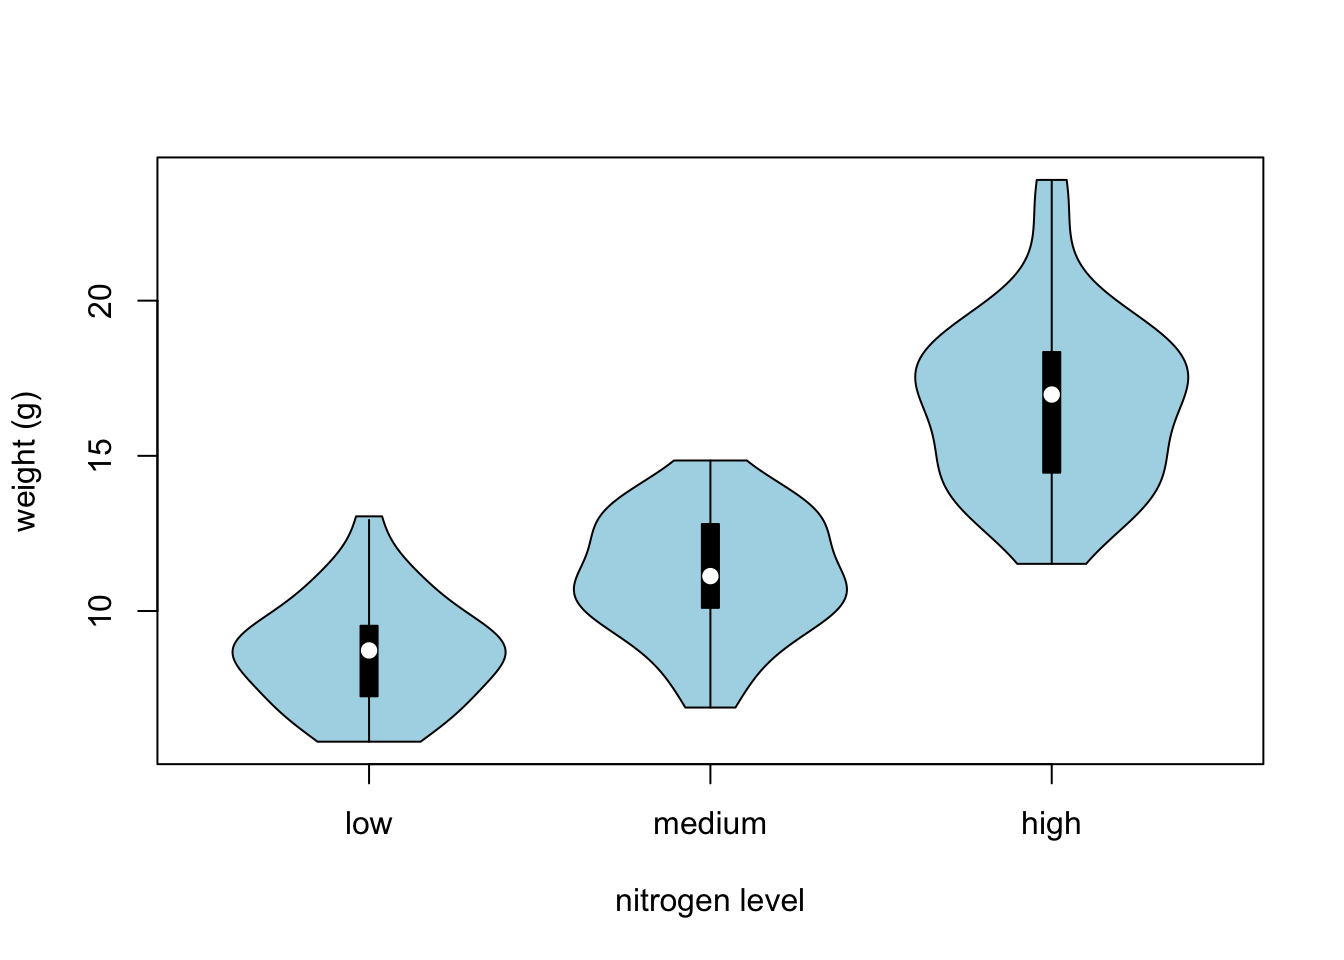
\includegraphics{05-R-Basic-Part5_files/figure-latex/unnamed-chunk-21-1.pdf}

\section*{Pairs plot}\label{pairs-plot}
\addcontentsline{toc}{section}{Pairs plot}

\begin{Shaded}
\begin{Highlighting}[]
\FunctionTok{plot}\NormalTok{(flowers)}
\end{Highlighting}
\end{Shaded}

\includegraphics{05-R-Basic-Part5_files/figure-latex/unnamed-chunk-22-1.pdf}

\begin{Shaded}
\begin{Highlighting}[]
\FunctionTok{pairs}\NormalTok{(flowers[, }\FunctionTok{c}\NormalTok{(}\StringTok{"height"}\NormalTok{, }\StringTok{"weight"}\NormalTok{, }\StringTok{"leafarea"}\NormalTok{, }
                \StringTok{"shootarea"}\NormalTok{, }\StringTok{"flowers"}\NormalTok{)])}
\end{Highlighting}
\end{Shaded}

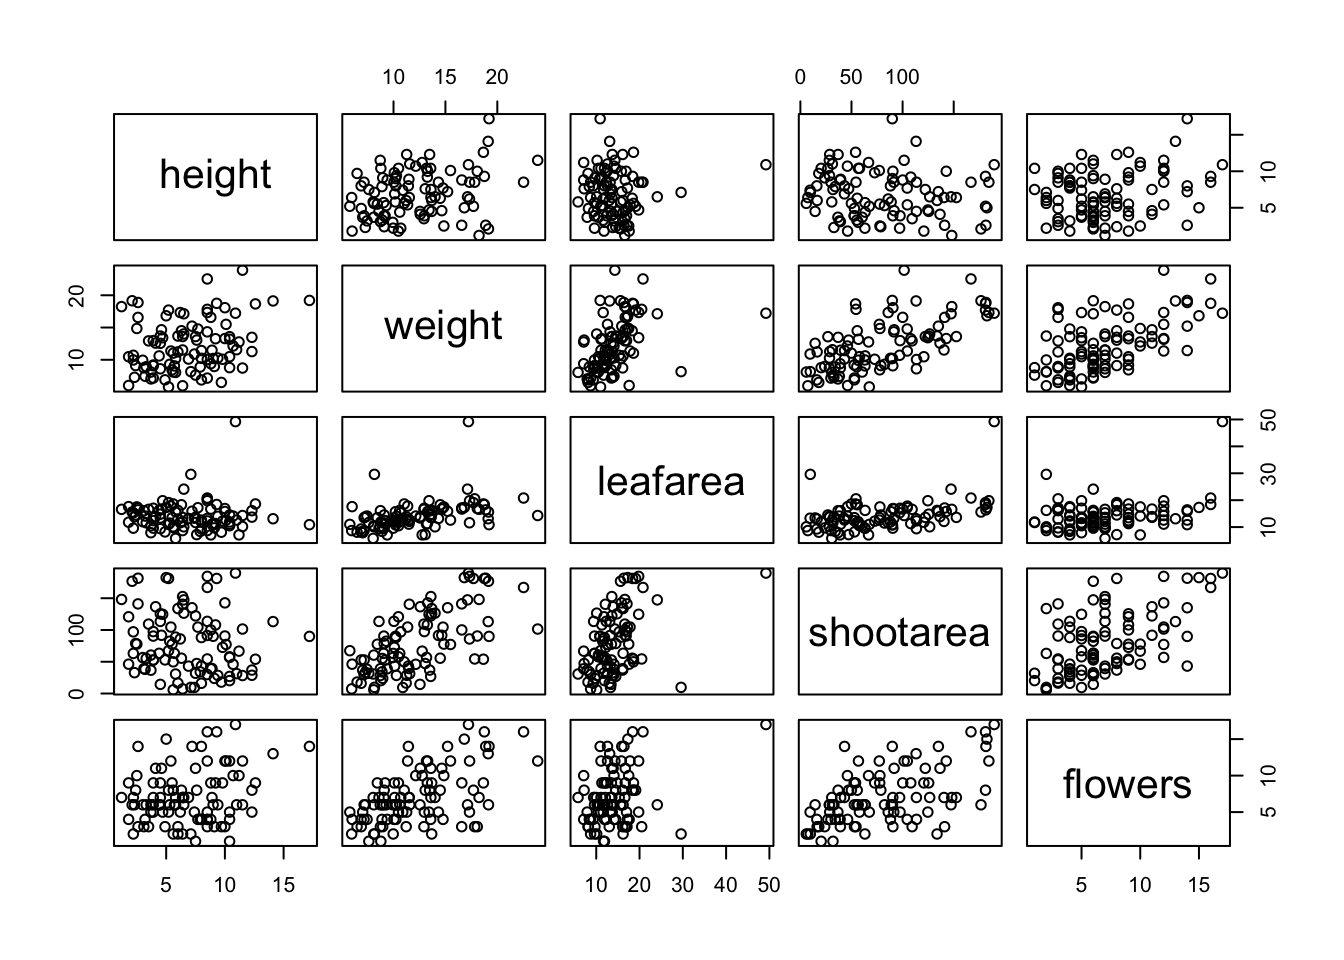
\includegraphics{05-R-Basic-Part5_files/figure-latex/unnamed-chunk-23-1.pdf}

\section*{Exercise 2}\label{exercise-2-2}
\addcontentsline{toc}{section}{Exercise 2}

Now, try creating your own visualization using the iris dataset. Here's what you can do:

\begin{enumerate}
\def\labelenumi{\arabic{enumi}.}
\tightlist
\item
  Create a scatter plot using Petal.Length and Petal.Width from the iris dataset.
\item
  Color the points based on the Species column to differentiate between the species.
\item
  Add a title, x-axis label, and y-axis label to your plot.
  Include a legend that indicates which color corresponds to which iris species.
\end{enumerate}

\chapter*{Intermediate R}\label{intermediate-r}
\addcontentsline{toc}{chapter}{Intermediate R}

In this session , we will learn about function and control structures such as writing functions , if statements, and loops.

We will also explore Data Cleaning and Transformations such as handling missing data , reshaping data using the dplyr functions.

First , we need to load this package

\begin{Shaded}
\begin{Highlighting}[]
\CommentTok{\#install.packages("tidyverse")}
\FunctionTok{library}\NormalTok{(tidyverse)}
\CommentTok{\#\textgreater{} {-}{-} Attaching core tidyverse packages {-}{-}{-}{-} tidyverse 2.0.0 {-}{-}}
\CommentTok{\#\textgreater{} v dplyr     1.1.4     v readr     2.1.4}
\CommentTok{\#\textgreater{} v forcats   1.0.0     v stringr   1.5.1}
\CommentTok{\#\textgreater{} v ggplot2   3.5.1     v tibble    3.2.1}
\CommentTok{\#\textgreater{} v lubridate 1.9.3     v tidyr     1.3.0}
\CommentTok{\#\textgreater{} v purrr     1.0.2     }
\CommentTok{\#\textgreater{} {-}{-} Conflicts {-}{-}{-}{-}{-}{-}{-}{-}{-}{-}{-}{-}{-}{-}{-}{-}{-}{-}{-}{-}{-}{-} tidyverse\_conflicts() {-}{-}}
\CommentTok{\#\textgreater{} x dplyr::filter() masks stats::filter()}
\CommentTok{\#\textgreater{} x dplyr::lag()    masks stats::lag()}
\CommentTok{\#\textgreater{} i Use the conflicted package (\textless{}http://conflicted.r{-}lib.org/\textgreater{}) to force all conflicts to become errors}
\end{Highlighting}
\end{Shaded}

It will load

\begin{enumerate}
\def\labelenumi{\arabic{enumi}.}
\tightlist
\item
  \texttt{ggplot2}: Used for data visualization using the grammar of graphics.
\item
  \texttt{dplyr}: Provides a set of tools for efficiently manipulating datasets.
\item
  \texttt{tidyr}: Used for tidying data, that is, transforming it to a format that is easy to work with.
\item
  \texttt{readr}: Used to read rectangular data like CSVs and text files into R.
\item
  \texttt{purrr}: Enhances R's functional programming (FP) toolkit, making it easier to work with lists and functions.
\item
  \texttt{tibble}: A modern reimagining of data frames, providing a cleaner and more user-friendly data structure.
\item
  \texttt{stringr}: Simplifies the process of working with strings (text data).
\item
  \texttt{forcats}: Designed to handle categorical variables (factors) with ease.
\end{enumerate}

In this session , we will use some of them

\chapter*{Part I: Functions and Control Structures}\label{part-i-functions-and-control-structures}
\addcontentsline{toc}{chapter}{Part I: Functions and Control Structures}

\section*{Writing and using functions}\label{writing-and-using-functions}
\addcontentsline{toc}{section}{Writing and using functions}

Example: A simple function to calculate the square of a number

\[
f(x) = x^2
\]

\begin{Shaded}
\begin{Highlighting}[]

\NormalTok{square\_function }\OtherTok{\textless{}{-}} \ControlFlowTok{function}\NormalTok{(x) \{}
  \FunctionTok{return}\NormalTok{(x}\SpecialCharTok{\^{}}\DecValTok{2}\NormalTok{)}
\NormalTok{\}}

\CommentTok{\# Using the function}
\NormalTok{result }\OtherTok{\textless{}{-}} \FunctionTok{square\_function}\NormalTok{(}\DecValTok{4}\NormalTok{)}
\FunctionTok{print}\NormalTok{(result)}
\CommentTok{\#\textgreater{} [1] 16}
\end{Highlighting}
\end{Shaded}

\subsection*{Exercise 1}\label{exercise-1-3}
\addcontentsline{toc}{subsection}{Exercise 1}

\textbf{Task:} Write and Use a Function
\textbf{Objective:} Create a function that calculates the cube of a number and use this function to calculate the cube of 3.

\textbf{Hint:} Use the structure of the square\_function as a template.

The reason why this is useful, is because functions are used for anything we want, R functions are just similar to the one we have just created, optimized for the specific tasks they were designed for .

We now create a more complex function , one that takes a vector , finds the mean , standard deviation and the histogram

\begin{Shaded}
\begin{Highlighting}[]
\NormalTok{analyze\_vector }\OtherTok{\textless{}{-}} \ControlFlowTok{function}\NormalTok{(x, }\AttributeTok{plot\_title =} \StringTok{"Histogram"}\NormalTok{) \{}
  \CommentTok{\# Check if the input is numeric}
  \ControlFlowTok{if}\NormalTok{ (}\SpecialCharTok{!}\FunctionTok{is.numeric}\NormalTok{(x)) \{}
    \FunctionTok{stop}\NormalTok{(}\StringTok{"Input must be a numeric vector"}\NormalTok{)}
\NormalTok{  \}}
  
  \CommentTok{\# Calculate mean and standard deviation}
\NormalTok{  mean\_value }\OtherTok{\textless{}{-}} \FunctionTok{mean}\NormalTok{(x)}
\NormalTok{  std\_value }\OtherTok{\textless{}{-}} \FunctionTok{sd}\NormalTok{(x)}
  
  \CommentTok{\# Output the mean and std}
  \FunctionTok{cat}\NormalTok{(}\StringTok{"Mean:"}\NormalTok{, mean\_value, }\StringTok{"}\SpecialCharTok{\textbackslash{}n}\StringTok{"}\NormalTok{)}
  \FunctionTok{cat}\NormalTok{(}\StringTok{"Standard Deviation:"}\NormalTok{, std\_value, }\StringTok{"}\SpecialCharTok{\textbackslash{}n}\StringTok{"}\NormalTok{)}
  
  \CommentTok{\# Create a histogram}
  \FunctionTok{hist}\NormalTok{(x, }\AttributeTok{main =}\NormalTok{ plot\_title, }\AttributeTok{xlab =} \StringTok{"Values"}\NormalTok{, }\AttributeTok{col =} \StringTok{"lightblue"}\NormalTok{, }\AttributeTok{border =} \StringTok{"black"}\NormalTok{)}
  
  \CommentTok{\# Return a list containing the mean and std}
  \FunctionTok{return}\NormalTok{(}\FunctionTok{list}\NormalTok{(}\AttributeTok{mean =}\NormalTok{ mean\_value, }\AttributeTok{std =}\NormalTok{ std\_value))}
\NormalTok{\}}

\CommentTok{\# Example usage with the mtcars$mpg vector}
\NormalTok{result }\OtherTok{\textless{}{-}} \FunctionTok{analyze\_vector}\NormalTok{(mtcars}\SpecialCharTok{$}\NormalTok{mpg, }\StringTok{"MPG Histogram"}\NormalTok{)}
\CommentTok{\#\textgreater{} Mean: 20.09062 }
\CommentTok{\#\textgreater{} Standard Deviation: 6.026948}
\end{Highlighting}
\end{Shaded}

\includegraphics{06-Intermediate-R-Part1_files/figure-latex/unnamed-chunk-3-1.pdf}

\subsection*{Exercise 2}\label{exercise-2-3}
\addcontentsline{toc}{subsection}{Exercise 2}

\textbf{Task:} Analyze a Numeric Vector
\textbf{Objective:} Write a function named summarize\_vector that takes a numeric vector as input and calculates the median, variance, and creates a boxplot. The function should print the median and variance, and return them as a list. Use the airquality\$Ozone data for analysis.

\textbf{Hint:} Similar to analyze\_vector, check if the input is numeric and use median, var, and \texttt{boxplot} functions.

\section*{If statements and loops (for and while)}\label{if-statements-and-loops-for-and-while}
\addcontentsline{toc}{section}{If statements and loops (for and while)}

\begin{Shaded}
\begin{Highlighting}[]
\CommentTok{\# Example: Using if statement}
\NormalTok{number }\OtherTok{\textless{}{-}} \DecValTok{5}
\ControlFlowTok{if}\NormalTok{ (number }\SpecialCharTok{\textgreater{}} \DecValTok{0}\NormalTok{) \{}
  \FunctionTok{print}\NormalTok{(}\StringTok{"Positive number"}\NormalTok{)}
\NormalTok{\} }\ControlFlowTok{else}\NormalTok{ \{}
  \FunctionTok{print}\NormalTok{(}\StringTok{"Non{-}positive number"}\NormalTok{)}
\NormalTok{\}}
\CommentTok{\#\textgreater{} [1] "Positive number"}
\end{Highlighting}
\end{Shaded}

\subsection*{Exercise 3}\label{exercise-3-1}
\addcontentsline{toc}{subsection}{Exercise 3}

\textbf{Task:} Using if Statements
\textbf{Objective:} Create an R script that checks if a number is negative, zero, or positive and prints an appropriate message. Test your script with the number -4.

\textbf{Hint:} Use an if statement followed by else if and else.

\section*{Example:}\label{example-6}
\addcontentsline{toc}{section}{Example:}

For loop to calculate the factorial of a number

\begin{Shaded}
\begin{Highlighting}[]

\NormalTok{factorial\_function }\OtherTok{\textless{}{-}} \ControlFlowTok{function}\NormalTok{(n) \{}
\NormalTok{  result }\OtherTok{\textless{}{-}} \DecValTok{1}
  \ControlFlowTok{for}\NormalTok{ (i }\ControlFlowTok{in} \DecValTok{1}\SpecialCharTok{:}\NormalTok{n) \{}
\NormalTok{    result }\OtherTok{\textless{}{-}}\NormalTok{ result }\SpecialCharTok{*}\NormalTok{ i}
\NormalTok{  \}}
  \FunctionTok{return}\NormalTok{(result)}
\NormalTok{\}}

\NormalTok{factorial\_of\_5 }\OtherTok{\textless{}{-}} \FunctionTok{factorial\_function}\NormalTok{(}\DecValTok{5}\NormalTok{)}
\FunctionTok{print}\NormalTok{(factorial\_of\_5)}
\CommentTok{\#\textgreater{} [1] 120}
\end{Highlighting}
\end{Shaded}

\subsection*{Exercise 4}\label{exercise-4-1}
\addcontentsline{toc}{subsection}{Exercise 4}

\textbf{Task:} For Loop
\textbf{Objective:} Write a function using a for loop that calculates the sum of squares of numbers from 1 to n.~Use this function to calculate the sum of squares for n=10.

\textbf{Hint:} Iterate from 1 to n, and keep adding the square of each number to a result variable.

\section*{Example:}\label{example-7}
\addcontentsline{toc}{section}{Example:}

While loop to find the first square number greater than 100

\begin{Shaded}
\begin{Highlighting}[]
\NormalTok{number }\OtherTok{\textless{}{-}} \DecValTok{1}
\ControlFlowTok{while}\NormalTok{ (number}\SpecialCharTok{\^{}}\DecValTok{2} \SpecialCharTok{\textless{}=} \DecValTok{100}\NormalTok{) \{}
\NormalTok{  number }\OtherTok{\textless{}{-}}\NormalTok{ number }\SpecialCharTok{+} \DecValTok{1}
\NormalTok{\}}
\FunctionTok{print}\NormalTok{(}\FunctionTok{paste}\NormalTok{(}\StringTok{"First square number greater than 100 is:"}\NormalTok{, number}\SpecialCharTok{\^{}}\DecValTok{2}\NormalTok{))}
\CommentTok{\#\textgreater{} [1] "First square number greater than 100 is: 121"}
\end{Highlighting}
\end{Shaded}

\subsection*{Exercise 5}\label{exercise-5-1}
\addcontentsline{toc}{subsection}{Exercise 5}

\textbf{Task:} While Loop
\textbf{Objective:} Write a script using a while loop that finds the smallest number whose cube is greater than 100. Print the number and its cube.

\textbf{Hint:} Increment a number starting from 1, and check if its cube is greater than 100 in the while loop condition.

\chapter*{Part II: Data Wrangling}\label{part-ii-data-wrangling}
\addcontentsline{toc}{chapter}{Part II: Data Wrangling}

Data wrangling, also known as data munging, is the process of
transforming and mapping data from one ``raw'' form into another format
with the intent of making it more appropriate and valuable for a variety
of downstream purposes, such as analytics.

In R, data wrangling is often performed using functions from the base R
language, as well as a collection of packages known as the tidyverse.
The tidyverse is a coherent system of packages for data manipulation,
exploration, and visualization that share a common design philosophy.

The tidyverse approach to data wrangling typically involves:

\begin{enumerate}
\def\labelenumi{\arabic{enumi}.}
\item
  Tidying Data: Transforming datasets into a consistent form that
  makes it easier to work with. This usually means converting data to
  a tidy format where each variable forms a column, each observation
  forms a row, and each type of observational unit forms a table.
\item
  Transforming Data: Once the data is tidy, a series of functions are
  used for data manipulation tasks such as selecting specific columns
  (select()), filtering for certain rows (filter()), creating new
  columns or modifying existing ones (mutate() or transmute()),
  summarizing data (summarise()), and reshaping data (pivot\_longer()
  and pivot\_wider()).
\item
  Working with Data Types and Structures: Functions from tidyverse
  allow for the easy manipulation of data types (like converting
  character vectors to factors with forcats) and data structures (like
  tibbles with the tibble package, which are a modern take on data
  frames).
\item
  Joining Data: Combining different datasets in a variety of ways
  (like left\_join(), right\_join(), inner\_join(), full\_join(), and
  anti\_join()) based on common keys or identifiers.
\item
  Handling Strings and Dates: The tidyverse includes packages like
  stringr for string operations and lubridate for dealing with
  date-time objects, which are essential in many data wrangling tasks.
\item
  Functional Programming: The package purrr introduces powerful
  functional programming tools to iterate over data structures and
  perform operations repeatedly.
\end{enumerate}

The primary goal of data wrangling is to ensure that the data is in the
best possible format for analysis. The tidyverse provides tools that
make these tasks straightforward, efficient, and often more intuitive
than the base R equivalents. The philosophy of the tidyverse is to write
readable and transparent code that can be understood even if you come
back to it months or years later.

\section*{Reshaping data using dplyr functions (filter, arrange, mutate, summarize)}\label{reshaping-data-using-dplyr-functions-filter-arrange-mutate-summarize}
\addcontentsline{toc}{section}{Reshaping data using dplyr functions (filter, arrange, mutate, summarize)}

The \texttt{dplyr} package was developed by Hadley Wickham of RStudio and is an
optimized and distilled version of his plyr package. The \texttt{dplyr} package
does not provide any ``new'' functionality to R per se, in the sense that
everything dplyr does could already be done with base R, but it greatly
simplifies existing functionality in R.

One important contribution of the \texttt{dplyr} package is that it provides a
``grammar'' (in particular, verbs) for data manipulation and for operating
on data frames. With this grammar, you can sensibly communicate what it
is that you are doing to a data frame that other people can understand
(assuming they also know the grammar). This is useful because it
provides an abstraction for data manipulation that previously did not
exist. Another useful contribution is that the \texttt{dplyr} functions are
very fast, as many key operations are coded in C++.

The \texttt{dplyr} grammar

Some of the key ``verbs'' provided by the dplyr package are

\begin{itemize}
\item
  select: return a subset of the columns of a data frame, using a
  flexible notation
\item
  filter: extract a subset of rows from a data frame based on logical
  conditions
\item
  arrange: reorder rows of a data frame
\item
  rename: rename variables in a data frame
\item
  mutate: add new variables/columns or transform existing variables
\item
  summarise / summarize: generate summary statistics of different
  variables in the data frame, possibly within strata
\item
  \texttt{\%\textgreater{}\%}: the ``pipe'' operator is used to connect multiple verb actions
  together into a pipeline.
\end{itemize}

These all combine naturally with group\_by() which allows you to perform
any operation ``by group''.

\subsection*{More on the pipe operator}\label{more-on-the-pipe-operator}
\addcontentsline{toc}{subsection}{More on the pipe operator}

\begin{itemize}
\tightlist
\item
  It takes the output of one statement and makes it the input of the
  next statement.
\item
  When describing it, you can think of it as a ``THEN''. A first
  example:

  \begin{itemize}
  \tightlist
  \item
    take the diamonds data (from the ggplot2 package)
  \item
    then subset
  \end{itemize}
\end{itemize}

\begin{Shaded}
\begin{Highlighting}[]
\FunctionTok{library}\NormalTok{(dplyr)}
\CommentTok{\#\textgreater{} }
\CommentTok{\#\textgreater{} Attaching package: \textquotesingle{}dplyr\textquotesingle{}}
\CommentTok{\#\textgreater{} The following objects are masked from \textquotesingle{}package:stats\textquotesingle{}:}
\CommentTok{\#\textgreater{} }
\CommentTok{\#\textgreater{}     filter, lag}
\CommentTok{\#\textgreater{} The following objects are masked from \textquotesingle{}package:base\textquotesingle{}:}
\CommentTok{\#\textgreater{} }
\CommentTok{\#\textgreater{}     intersect, setdiff, setequal, union}
\FunctionTok{library}\NormalTok{(ggplot2)}
\NormalTok{diamonds }\SpecialCharTok{\%\textgreater{}\%} \FunctionTok{filter}\NormalTok{(cut }\SpecialCharTok{==} \StringTok{"Ideal"}\NormalTok{)}
\CommentTok{\#\textgreater{} \# A tibble: 21,551 x 10}
\CommentTok{\#\textgreater{}    carat cut   color clarity depth table price     x     y}
\CommentTok{\#\textgreater{}    \textless{}dbl\textgreater{} \textless{}ord\textgreater{} \textless{}ord\textgreater{} \textless{}ord\textgreater{}   \textless{}dbl\textgreater{} \textless{}dbl\textgreater{} \textless{}int\textgreater{} \textless{}dbl\textgreater{} \textless{}dbl\textgreater{}}
\CommentTok{\#\textgreater{}  1  0.23 Ideal E     SI2      61.5    55   326  3.95  3.98}
\CommentTok{\#\textgreater{}  2  0.23 Ideal J     VS1      62.8    56   340  3.93  3.9 }
\CommentTok{\#\textgreater{}  3  0.31 Ideal J     SI2      62.2    54   344  4.35  4.37}
\CommentTok{\#\textgreater{}  4  0.3  Ideal I     SI2      62      54   348  4.31  4.34}
\CommentTok{\#\textgreater{}  5  0.33 Ideal I     SI2      61.8    55   403  4.49  4.51}
\CommentTok{\#\textgreater{}  6  0.33 Ideal I     SI2      61.2    56   403  4.49  4.5 }
\CommentTok{\#\textgreater{}  7  0.33 Ideal J     SI1      61.1    56   403  4.49  4.55}
\CommentTok{\#\textgreater{}  8  0.23 Ideal G     VS1      61.9    54   404  3.93  3.95}
\CommentTok{\#\textgreater{}  9  0.32 Ideal I     SI1      60.9    55   404  4.45  4.48}
\CommentTok{\#\textgreater{} 10  0.3  Ideal I     SI2      61      59   405  4.3   4.33}
\CommentTok{\#\textgreater{} \# i 21,541 more rows}
\CommentTok{\#\textgreater{} \# i 1 more variable: z \textless{}dbl\textgreater{}}
\end{Highlighting}
\end{Shaded}

\subsection*{Filter()}\label{filter}
\addcontentsline{toc}{subsection}{Filter()}

Extract rows that meet logical criteria. Here you go: - inspect the
diamonds data set - filter observations with cut equal to Ideal

\begin{Shaded}
\begin{Highlighting}[]
\FunctionTok{filter}\NormalTok{(diamonds, cut }\SpecialCharTok{==} \StringTok{"Ideal"}\NormalTok{)}
\CommentTok{\#\textgreater{} \# A tibble: 21,551 x 10}
\CommentTok{\#\textgreater{}    carat cut   color clarity depth table price     x     y}
\CommentTok{\#\textgreater{}    \textless{}dbl\textgreater{} \textless{}ord\textgreater{} \textless{}ord\textgreater{} \textless{}ord\textgreater{}   \textless{}dbl\textgreater{} \textless{}dbl\textgreater{} \textless{}int\textgreater{} \textless{}dbl\textgreater{} \textless{}dbl\textgreater{}}
\CommentTok{\#\textgreater{}  1  0.23 Ideal E     SI2      61.5    55   326  3.95  3.98}
\CommentTok{\#\textgreater{}  2  0.23 Ideal J     VS1      62.8    56   340  3.93  3.9 }
\CommentTok{\#\textgreater{}  3  0.31 Ideal J     SI2      62.2    54   344  4.35  4.37}
\CommentTok{\#\textgreater{}  4  0.3  Ideal I     SI2      62      54   348  4.31  4.34}
\CommentTok{\#\textgreater{}  5  0.33 Ideal I     SI2      61.8    55   403  4.49  4.51}
\CommentTok{\#\textgreater{}  6  0.33 Ideal I     SI2      61.2    56   403  4.49  4.5 }
\CommentTok{\#\textgreater{}  7  0.33 Ideal J     SI1      61.1    56   403  4.49  4.55}
\CommentTok{\#\textgreater{}  8  0.23 Ideal G     VS1      61.9    54   404  3.93  3.95}
\CommentTok{\#\textgreater{}  9  0.32 Ideal I     SI1      60.9    55   404  4.45  4.48}
\CommentTok{\#\textgreater{} 10  0.3  Ideal I     SI2      61      59   405  4.3   4.33}
\CommentTok{\#\textgreater{} \# i 21,541 more rows}
\CommentTok{\#\textgreater{} \# i 1 more variable: z \textless{}dbl\textgreater{}}
\end{Highlighting}
\end{Shaded}

\subsection*{Overview of logical tests}\label{overview-of-logical-tests}
\addcontentsline{toc}{subsection}{Overview of logical tests}

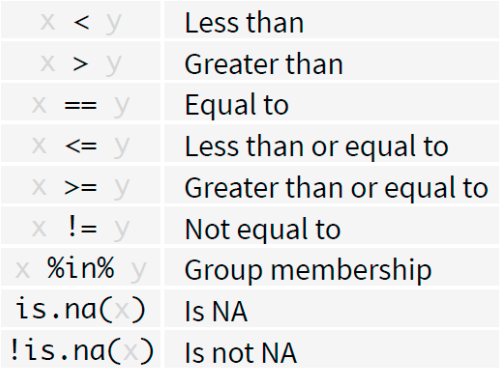
\includegraphics[width=0.4\linewidth,height=0.2\textheight]{images/logical_tests}

\section*{Mutate()}\label{mutate}
\addcontentsline{toc}{section}{Mutate()}

Create new columns. Here you go: - inspect the diamonds data set -
create a new variable price\_per\_carat

\begin{Shaded}
\begin{Highlighting}[]
\FunctionTok{mutate}\NormalTok{(diamonds, }\AttributeTok{price\_per\_carat =}\NormalTok{ price}\SpecialCharTok{/}\NormalTok{carat)}
\CommentTok{\#\textgreater{} \# A tibble: 53,940 x 11}
\CommentTok{\#\textgreater{}    carat cut     color clarity depth table price     x     y}
\CommentTok{\#\textgreater{}    \textless{}dbl\textgreater{} \textless{}ord\textgreater{}   \textless{}ord\textgreater{} \textless{}ord\textgreater{}   \textless{}dbl\textgreater{} \textless{}dbl\textgreater{} \textless{}int\textgreater{} \textless{}dbl\textgreater{} \textless{}dbl\textgreater{}}
\CommentTok{\#\textgreater{}  1  0.23 Ideal   E     SI2      61.5    55   326  3.95  3.98}
\CommentTok{\#\textgreater{}  2  0.21 Premium E     SI1      59.8    61   326  3.89  3.84}
\CommentTok{\#\textgreater{}  3  0.23 Good    E     VS1      56.9    65   327  4.05  4.07}
\CommentTok{\#\textgreater{}  4  0.29 Premium I     VS2      62.4    58   334  4.2   4.23}
\CommentTok{\#\textgreater{}  5  0.31 Good    J     SI2      63.3    58   335  4.34  4.35}
\CommentTok{\#\textgreater{}  6  0.24 Very G\textasciitilde{} J     VVS2     62.8    57   336  3.94  3.96}
\CommentTok{\#\textgreater{}  7  0.24 Very G\textasciitilde{} I     VVS1     62.3    57   336  3.95  3.98}
\CommentTok{\#\textgreater{}  8  0.26 Very G\textasciitilde{} H     SI1      61.9    55   337  4.07  4.11}
\CommentTok{\#\textgreater{}  9  0.22 Fair    E     VS2      65.1    61   337  3.87  3.78}
\CommentTok{\#\textgreater{} 10  0.23 Very G\textasciitilde{} H     VS1      59.4    61   338  4     4.05}
\CommentTok{\#\textgreater{} \# i 53,930 more rows}
\CommentTok{\#\textgreater{} \# i 2 more variables: z \textless{}dbl\textgreater{}, price\_per\_carat \textless{}dbl\textgreater{}}
\end{Highlighting}
\end{Shaded}

\section*{Multistep operations}\label{multistep-operations}
\addcontentsline{toc}{section}{Multistep operations}

Use the \%\textgreater\% for multistep operations. Passes result on left into first
argument of function on right. Here you go:

\begin{Shaded}
\begin{Highlighting}[]
\NormalTok{diamonds }\SpecialCharTok{\%\textgreater{}\%} 
  \FunctionTok{mutate}\NormalTok{(}\AttributeTok{price\_per\_carat =}\NormalTok{ price}\SpecialCharTok{/}\NormalTok{carat)  }\SpecialCharTok{\%\textgreater{}\%}
  \FunctionTok{filter}\NormalTok{(price\_per\_carat }\SpecialCharTok{\textgreater{}} \DecValTok{1500}\NormalTok{)}
\CommentTok{\#\textgreater{} \# A tibble: 52,821 x 11}
\CommentTok{\#\textgreater{}    carat cut     color clarity depth table price     x     y}
\CommentTok{\#\textgreater{}    \textless{}dbl\textgreater{} \textless{}ord\textgreater{}   \textless{}ord\textgreater{} \textless{}ord\textgreater{}   \textless{}dbl\textgreater{} \textless{}dbl\textgreater{} \textless{}int\textgreater{} \textless{}dbl\textgreater{} \textless{}dbl\textgreater{}}
\CommentTok{\#\textgreater{}  1  0.21 Premium E     SI1      59.8    61   326  3.89  3.84}
\CommentTok{\#\textgreater{}  2  0.22 Fair    E     VS2      65.1    61   337  3.87  3.78}
\CommentTok{\#\textgreater{}  3  0.22 Premium F     SI1      60.4    61   342  3.88  3.84}
\CommentTok{\#\textgreater{}  4  0.2  Premium E     SI2      60.2    62   345  3.79  3.75}
\CommentTok{\#\textgreater{}  5  0.23 Very G\textasciitilde{} E     VS2      63.8    55   352  3.85  3.92}
\CommentTok{\#\textgreater{}  6  0.23 Very G\textasciitilde{} H     VS1      61      57   353  3.94  3.96}
\CommentTok{\#\textgreater{}  7  0.23 Very G\textasciitilde{} G     VVS2     60.4    58   354  3.97  4.01}
\CommentTok{\#\textgreater{}  8  0.23 Very G\textasciitilde{} D     VS2      60.5    61   357  3.96  3.97}
\CommentTok{\#\textgreater{}  9  0.23 Very G\textasciitilde{} F     VS1      60.9    57   357  3.96  3.99}
\CommentTok{\#\textgreater{} 10  0.23 Very G\textasciitilde{} F     VS1      60      57   402  4     4.03}
\CommentTok{\#\textgreater{} \# i 52,811 more rows}
\CommentTok{\#\textgreater{} \# i 2 more variables: z \textless{}dbl\textgreater{}, price\_per\_carat \textless{}dbl\textgreater{}}
\end{Highlighting}
\end{Shaded}

\section*{Summarize()}\label{summarize}
\addcontentsline{toc}{section}{Summarize()}

Compute table of summaries. Here you go:

\begin{itemize}
\tightlist
\item
  inspect the diamonds data set
\item
  calculate mean and standard deviation of price
\end{itemize}

\begin{Shaded}
\begin{Highlighting}[]
\NormalTok{diamonds }\SpecialCharTok{\%\textgreater{}\%} \FunctionTok{summarize}\NormalTok{(}\AttributeTok{mean =} \FunctionTok{mean}\NormalTok{(price), }\AttributeTok{std\_dev =} \FunctionTok{sd}\NormalTok{(price))}
\CommentTok{\#\textgreater{} \# A tibble: 1 x 2}
\CommentTok{\#\textgreater{}    mean std\_dev}
\CommentTok{\#\textgreater{}   \textless{}dbl\textgreater{}   \textless{}dbl\textgreater{}}
\CommentTok{\#\textgreater{} 1 3933.   3989.}
\end{Highlighting}
\end{Shaded}

\section*{Group\_by()}\label{group_by}
\addcontentsline{toc}{section}{Group\_by()}

Groups cases by common values of one or more columns. Here you go:
inspect the diamonds data set calculate mean and standard deviation of
price by level of cut

\begin{Shaded}
\begin{Highlighting}[]
\NormalTok{diamonds }\SpecialCharTok{\%\textgreater{}\%} 
        \FunctionTok{group\_by}\NormalTok{(cut) }\SpecialCharTok{\%\textgreater{}\%} 
        \FunctionTok{summarize}\NormalTok{(}\AttributeTok{price =} \FunctionTok{mean}\NormalTok{(price), }\AttributeTok{carat =} \FunctionTok{mean}\NormalTok{(carat))}
\CommentTok{\#\textgreater{} \# A tibble: 5 x 3}
\CommentTok{\#\textgreater{}   cut       price carat}
\CommentTok{\#\textgreater{}   \textless{}ord\textgreater{}     \textless{}dbl\textgreater{} \textless{}dbl\textgreater{}}
\CommentTok{\#\textgreater{} 1 Fair      4359. 1.05 }
\CommentTok{\#\textgreater{} 2 Good      3929. 0.849}
\CommentTok{\#\textgreater{} 3 Very Good 3982. 0.806}
\CommentTok{\#\textgreater{} 4 Premium   4584. 0.892}
\CommentTok{\#\textgreater{} 5 Ideal     3458. 0.703}
\end{Highlighting}
\end{Shaded}

\subsection*{Exercise 1}\label{exercise-1-4}
\addcontentsline{toc}{subsection}{Exercise 1}

\begin{enumerate}
\def\labelenumi{\arabic{enumi}.}
\tightlist
\item
  Load the data Parade2005.txt.
\item
  Determine the mean earnings in California.
\item
  Determine the number of individuals residing in Idaho.
\item
  Determine the mean and the median earnings of celebrities.
\end{enumerate}

\section*{Transforming a dataframe into tibbles}\label{transforming-a-dataframe-into-tibbles}
\addcontentsline{toc}{section}{Transforming a dataframe into tibbles}

Transform the mtcars into a tibble and inspect.

\begin{Shaded}
\begin{Highlighting}[]
\FunctionTok{str}\NormalTok{(mtcars)}
\CommentTok{\#\textgreater{} \textquotesingle{}data.frame\textquotesingle{}:    32 obs. of  11 variables:}
\CommentTok{\#\textgreater{}  $ mpg : num  21 21 22.8 21.4 18.7 18.1 14.3 24.4 22.8 19.2 ...}
\CommentTok{\#\textgreater{}  $ cyl : num  6 6 4 6 8 6 8 4 4 6 ...}
\CommentTok{\#\textgreater{}  $ disp: num  160 160 108 258 360 ...}
\CommentTok{\#\textgreater{}  $ hp  : num  110 110 93 110 175 105 245 62 95 123 ...}
\CommentTok{\#\textgreater{}  $ drat: num  3.9 3.9 3.85 3.08 3.15 2.76 3.21 3.69 3.92 3.92 ...}
\CommentTok{\#\textgreater{}  $ wt  : num  2.62 2.88 2.32 3.21 3.44 ...}
\CommentTok{\#\textgreater{}  $ qsec: num  16.5 17 18.6 19.4 17 ...}
\CommentTok{\#\textgreater{}  $ vs  : num  0 0 1 1 0 1 0 1 1 1 ...}
\CommentTok{\#\textgreater{}  $ am  : num  1 1 1 0 0 0 0 0 0 0 ...}
\CommentTok{\#\textgreater{}  $ gear: num  4 4 4 3 3 3 3 4 4 4 ...}
\CommentTok{\#\textgreater{}  $ carb: num  4 4 1 1 2 1 4 2 2 4 ...}
\end{Highlighting}
\end{Shaded}

\begin{Shaded}
\begin{Highlighting}[]
\CommentTok{\#library(tidyverse)}
\FunctionTok{library}\NormalTok{(tibble)}
\FunctionTok{as\_tibble}\NormalTok{(mtcars)}
\CommentTok{\#\textgreater{} \# A tibble: 32 x 11}
\CommentTok{\#\textgreater{}      mpg   cyl  disp    hp  drat    wt  qsec    vs    am}
\CommentTok{\#\textgreater{}    \textless{}dbl\textgreater{} \textless{}dbl\textgreater{} \textless{}dbl\textgreater{} \textless{}dbl\textgreater{} \textless{}dbl\textgreater{} \textless{}dbl\textgreater{} \textless{}dbl\textgreater{} \textless{}dbl\textgreater{} \textless{}dbl\textgreater{}}
\CommentTok{\#\textgreater{}  1  21       6  160    110  3.9   2.62  16.5     0     1}
\CommentTok{\#\textgreater{}  2  21       6  160    110  3.9   2.88  17.0     0     1}
\CommentTok{\#\textgreater{}  3  22.8     4  108     93  3.85  2.32  18.6     1     1}
\CommentTok{\#\textgreater{}  4  21.4     6  258    110  3.08  3.22  19.4     1     0}
\CommentTok{\#\textgreater{}  5  18.7     8  360    175  3.15  3.44  17.0     0     0}
\CommentTok{\#\textgreater{}  6  18.1     6  225    105  2.76  3.46  20.2     1     0}
\CommentTok{\#\textgreater{}  7  14.3     8  360    245  3.21  3.57  15.8     0     0}
\CommentTok{\#\textgreater{}  8  24.4     4  147.    62  3.69  3.19  20       1     0}
\CommentTok{\#\textgreater{}  9  22.8     4  141.    95  3.92  3.15  22.9     1     0}
\CommentTok{\#\textgreater{} 10  19.2     6  168.   123  3.92  3.44  18.3     1     0}
\CommentTok{\#\textgreater{} \# i 22 more rows}
\CommentTok{\#\textgreater{} \# i 2 more variables: gear \textless{}dbl\textgreater{}, carb \textless{}dbl\textgreater{}}
\end{Highlighting}
\end{Shaded}

\section*{Part II : Data Cleaning and Transformation}\label{part-ii-data-cleaning-and-transformation}
\addcontentsline{toc}{section}{Part II : Data Cleaning and Transformation}

Data cleaning is a fundamental step in the data analysis process, aimed
at improving data quality and ensuring its appropriateness for specific
analytical tasks. The process involves identifying and rectifying errors
or inconsistencies in data to enhance its accuracy, completeness, and
reliability.

Key aspects of data cleaning include:

\begin{itemize}
\item
  \textbf{Removing Duplicates}: This involves detecting and eliminating
  duplicate records that could skew analysis results.
\item
  \textbf{Handling Missing Dat}a: Missing values can be dealt with by
  imputing data (filling in missing values using statistical methods
  or domain knowledge), or in some cases, deleting rows or columns
  with too many missing values.
\item
  \textbf{Correcting Errors}: This involves identifying outliers or
  incorrect entries (due to data entry errors, measurement errors,
  etc.) and correcting them based on context or predefined rules.
\item
  \textbf{Standardizing Formats}: Ensuring that data across different
  sources or fields conforms to a consistent format, such as
  converting all dates to the same format, standardizing text entries
  (capitalization, removing leading/trailing spaces), or ensuring
  consistent measurement units.
\item
  \textbf{Filtering Irrelevant Information}: Removing data that is not
  relevant to the specific analysis task to focus on more significant
  data.
\item
  \textbf{Validating Accuracy}: Checking data against known standards or
  validation rules to ensure it correctly represents the real-world
  constructs it is supposed to reflect.
\item
  \textbf{Consolidating Data Sources}: Combining data from multiple sources
  and ensuring that the combined dataset is coherent and correctly
  integrated.
\end{itemize}

The aim of data cleaning is not only to correct errors but also to bring
structure and order to the data, facilitating more effective and
accurate analysis. By cleaning data, analysts can ensure that their
insights and conclusions are based on reliable and valid data, which is
crucial for making informed decisions.

\section*{The Policy data set}\label{the-policy-data-set}
\addcontentsline{toc}{section}{The Policy data set}

\begin{itemize}
\tightlist
\item
  PolicyData.csv available in the course material
\item
  Data stored in a .csv file.
\item
  Individual records separated by a semicolon.
\end{itemize}

\begin{Shaded}
\begin{Highlighting}[]
\NormalTok{policy\_data }\OtherTok{\textless{}{-}} \FunctionTok{read.csv}\NormalTok{(}\AttributeTok{file =} \StringTok{\textquotesingle{}./Data/PolicyData.csv\textquotesingle{}}\NormalTok{, }\AttributeTok{sep =} \StringTok{\textquotesingle{};\textquotesingle{}}\NormalTok{)}
\end{Highlighting}
\end{Shaded}

\subsection*{Exercise 1}\label{exercise-1-5}
\addcontentsline{toc}{subsection}{Exercise 1}

Use the skills you obtained in the first R workshop and Part 1

\begin{enumerate}
\def\labelenumi{\arabic{enumi}.}
\tightlist
\item
  Inspect the top rows of the data set.
\item
  How many observations does the data set contain?
\item
  Calculate the total exposure (exposition) in each region
  (type\_territoire).
\end{enumerate}

\section*{The Gapminder package}\label{the-gapminder-package}
\addcontentsline{toc}{section}{The Gapminder package}

\begin{itemize}
\tightlist
\item
  Describes the evolution of a number of population characteristics
  (GDP, life expectancy, \ldots) over time.
\end{itemize}

\begin{Shaded}
\begin{Highlighting}[]
\CommentTok{\#install.packages("gapminder")}
\FunctionTok{library}\NormalTok{(gapminder)}
\end{Highlighting}
\end{Shaded}

\subsection*{Exercise 2}\label{exercise-2-4}
\addcontentsline{toc}{subsection}{Exercise 2}

Use the skills obtained in Part I:

\begin{enumerate}
\def\labelenumi{\arabic{enumi}.}
\tightlist
\item
  Inspect the top rows of the data.
\item
  Select the data for countries in Asia.
\item
  Which type of variable is \texttt{country}?
\end{enumerate}

\section*{Revisit factor()}\label{revisit-factor}
\addcontentsline{toc}{section}{Revisit factor()}

\subsection*{What is a factor variable ?}\label{what-is-a-factor-variable}
\addcontentsline{toc}{subsection}{What is a factor variable ?}

\begin{itemize}
\tightlist
\item
  Representation for categorical data.
\item
  Predefined list of outcomes (levels).
\item
  Protecting data quality.
\end{itemize}

Example , sex a categorical value with two possible outcomes, \texttt{m} and
\texttt{f}

\begin{Shaded}
\begin{Highlighting}[]
\NormalTok{sex }\OtherTok{\textless{}{-}} \FunctionTok{factor}\NormalTok{(}\FunctionTok{c}\NormalTok{(}\StringTok{\textquotesingle{}m\textquotesingle{}}\NormalTok{, }\StringTok{\textquotesingle{}f\textquotesingle{}}\NormalTok{, }\StringTok{\textquotesingle{}m\textquotesingle{}}\NormalTok{, }\StringTok{\textquotesingle{}f\textquotesingle{}}\NormalTok{),}
              \AttributeTok{levels =} \FunctionTok{c}\NormalTok{(}\StringTok{\textquotesingle{}m\textquotesingle{}}\NormalTok{, }\StringTok{\textquotesingle{}f\textquotesingle{}}\NormalTok{))}
\NormalTok{sex}
\CommentTok{\#\textgreater{} [1] m f m f}
\CommentTok{\#\textgreater{} Levels: m f}
\end{Highlighting}
\end{Shaded}

\begin{itemize}
\item
  The \texttt{factor} command creates a new factor variable. The first input
  is the categorical variable.
\item
  \texttt{levels} specifies the possible outcomes of the variable.
\end{itemize}

Assigning an unrecognized level to a factor variable results in a
warning

\begin{Shaded}
\begin{Highlighting}[]
\NormalTok{sex[}\DecValTok{1}\NormalTok{] }\OtherTok{\textless{}{-}} \StringTok{\textquotesingle{}male\textquotesingle{}}
\CommentTok{\#\textgreater{} Warning in \textasciigrave{}[\textless{}{-}.factor\textasciigrave{}(\textasciigrave{}*tmp*\textasciigrave{}, 1, value = "male"):}
\CommentTok{\#\textgreater{} invalid factor level, NA generated}
\end{Highlighting}
\end{Shaded}

This protects the quality of the data

\begin{Shaded}
\begin{Highlighting}[]
\NormalTok{sex}
\CommentTok{\#\textgreater{} [1] \textless{}NA\textgreater{} f    m    f   }
\CommentTok{\#\textgreater{} Levels: m f}
\end{Highlighting}
\end{Shaded}

The value NA is assigned to the invalid observation.

\section*{levels()}\label{levels}
\addcontentsline{toc}{section}{levels()}

levels print the allowed outcomes for a factor variable

\begin{Shaded}
\begin{Highlighting}[]
\FunctionTok{levels}\NormalTok{(sex)}
\CommentTok{\#\textgreater{} [1] "m" "f"}
\end{Highlighting}
\end{Shaded}

Assigning a vector to levels() renames the allowed outcomes.

\begin{Shaded}
\begin{Highlighting}[]
\FunctionTok{levels}\NormalTok{(sex) }\OtherTok{\textless{}{-}} \FunctionTok{c}\NormalTok{(}\StringTok{\textquotesingle{}male\textquotesingle{}}\NormalTok{, }\StringTok{\textquotesingle{}female\textquotesingle{}}\NormalTok{)}
\NormalTok{sex}
\CommentTok{\#\textgreater{} [1] \textless{}NA\textgreater{}   female male   female}
\CommentTok{\#\textgreater{} Levels: male female}
\end{Highlighting}
\end{Shaded}

\subsection*{Exercise 4}\label{exercise-4-2}
\addcontentsline{toc}{subsection}{Exercise 4}

The variable country in the gapminder data set is a factor variable.

\begin{enumerate}
\def\labelenumi{\arabic{enumi}.}
\tightlist
\item
  What are the possible levels for country in the subset asia.
\item
  Is this the result you expected?
\end{enumerate}

To add a level

\begin{Shaded}
\begin{Highlighting}[]
\FunctionTok{levels}\NormalTok{(sex) }\OtherTok{\textless{}{-}} \FunctionTok{c}\NormalTok{(}\FunctionTok{levels}\NormalTok{(sex), }\StringTok{\textquotesingle{}x\textquotesingle{}}\NormalTok{)}
\end{Highlighting}
\end{Shaded}

\section*{cut()}\label{cut}
\addcontentsline{toc}{section}{cut()}

\begin{Shaded}
\begin{Highlighting}[]
\NormalTok{gapminder}
\CommentTok{\#\textgreater{} \# A tibble: 1,704 x 6}
\CommentTok{\#\textgreater{}    country     continent  year lifeExp      pop gdpPercap}
\CommentTok{\#\textgreater{}    \textless{}fct\textgreater{}       \textless{}fct\textgreater{}     \textless{}int\textgreater{}   \textless{}dbl\textgreater{}    \textless{}int\textgreater{}     \textless{}dbl\textgreater{}}
\CommentTok{\#\textgreater{}  1 Afghanistan Asia       1952    28.8  8425333      779.}
\CommentTok{\#\textgreater{}  2 Afghanistan Asia       1957    30.3  9240934      821.}
\CommentTok{\#\textgreater{}  3 Afghanistan Asia       1962    32.0 10267083      853.}
\CommentTok{\#\textgreater{}  4 Afghanistan Asia       1967    34.0 11537966      836.}
\CommentTok{\#\textgreater{}  5 Afghanistan Asia       1972    36.1 13079460      740.}
\CommentTok{\#\textgreater{}  6 Afghanistan Asia       1977    38.4 14880372      786.}
\CommentTok{\#\textgreater{}  7 Afghanistan Asia       1982    39.9 12881816      978.}
\CommentTok{\#\textgreater{}  8 Afghanistan Asia       1987    40.8 13867957      852.}
\CommentTok{\#\textgreater{}  9 Afghanistan Asia       1992    41.7 16317921      649.}
\CommentTok{\#\textgreater{} 10 Afghanistan Asia       1997    41.8 22227415      635.}
\CommentTok{\#\textgreater{} \# i 1,694 more rows}
\end{Highlighting}
\end{Shaded}

\begin{Shaded}
\begin{Highlighting}[]
\FunctionTok{head}\NormalTok{(}\FunctionTok{cut}\NormalTok{(gapminder}\SpecialCharTok{$}\NormalTok{pop,}
    \AttributeTok{breaks =} \FunctionTok{c}\NormalTok{(}\DecValTok{0}\NormalTok{, }\DecValTok{10}\SpecialCharTok{\^{}}\DecValTok{7}\NormalTok{, }\DecValTok{5}\SpecialCharTok{*}\DecValTok{10}\SpecialCharTok{\^{}}\DecValTok{7}\NormalTok{, }\DecValTok{10}\SpecialCharTok{\^{}}\DecValTok{8}\NormalTok{, }\ConstantTok{Inf}\NormalTok{)))}
\CommentTok{\#\textgreater{} [1] (0,1e+07]     (0,1e+07]     (1e+07,5e+07] (1e+07,5e+07]}
\CommentTok{\#\textgreater{} [5] (1e+07,5e+07] (1e+07,5e+07]}
\CommentTok{\#\textgreater{} 4 Levels: (0,1e+07] (1e+07,5e+07] ... (1e+08,Inf]}
\end{Highlighting}
\end{Shaded}

\begin{Shaded}
\begin{Highlighting}[]
\NormalTok{gapminder}\SpecialCharTok{$}\NormalTok{pop\_category }\OtherTok{=} \FunctionTok{cut}\NormalTok{(gapminder}\SpecialCharTok{$}\NormalTok{pop,}
                             \AttributeTok{breaks =} \FunctionTok{c}\NormalTok{(}\DecValTok{0}\NormalTok{, }\DecValTok{10}\SpecialCharTok{\^{}}\DecValTok{7}\NormalTok{, }\DecValTok{5}\SpecialCharTok{*}\DecValTok{10}\SpecialCharTok{\^{}}\DecValTok{7}\NormalTok{, }\DecValTok{10}\SpecialCharTok{\^{}}\DecValTok{8}\NormalTok{, }\ConstantTok{Inf}\NormalTok{),}
                             \AttributeTok{labels =} \FunctionTok{c}\NormalTok{(}\StringTok{"\textless{}= 10M"}\NormalTok{, }\StringTok{"10M{-}50M"}\NormalTok{, }\StringTok{"50M{-}100M"}\NormalTok{, }\StringTok{"\textgreater{} 100M"}\NormalTok{))}
\end{Highlighting}
\end{Shaded}

\begin{Shaded}
\begin{Highlighting}[]
\NormalTok{gapminder}
\CommentTok{\#\textgreater{} \# A tibble: 1,704 x 7}
\CommentTok{\#\textgreater{}    country     continent  year lifeExp      pop gdpPercap}
\CommentTok{\#\textgreater{}    \textless{}fct\textgreater{}       \textless{}fct\textgreater{}     \textless{}int\textgreater{}   \textless{}dbl\textgreater{}    \textless{}int\textgreater{}     \textless{}dbl\textgreater{}}
\CommentTok{\#\textgreater{}  1 Afghanistan Asia       1952    28.8  8425333      779.}
\CommentTok{\#\textgreater{}  2 Afghanistan Asia       1957    30.3  9240934      821.}
\CommentTok{\#\textgreater{}  3 Afghanistan Asia       1962    32.0 10267083      853.}
\CommentTok{\#\textgreater{}  4 Afghanistan Asia       1967    34.0 11537966      836.}
\CommentTok{\#\textgreater{}  5 Afghanistan Asia       1972    36.1 13079460      740.}
\CommentTok{\#\textgreater{}  6 Afghanistan Asia       1977    38.4 14880372      786.}
\CommentTok{\#\textgreater{}  7 Afghanistan Asia       1982    39.9 12881816      978.}
\CommentTok{\#\textgreater{}  8 Afghanistan Asia       1987    40.8 13867957      852.}
\CommentTok{\#\textgreater{}  9 Afghanistan Asia       1992    41.7 16317921      649.}
\CommentTok{\#\textgreater{} 10 Afghanistan Asia       1997    41.8 22227415      635.}
\CommentTok{\#\textgreater{} \# i 1,694 more rows}
\CommentTok{\#\textgreater{} \# i 1 more variable: pop\_category \textless{}fct\textgreater{}}
\end{Highlighting}
\end{Shaded}

\section*{Exercise 5}\label{exercise-5-2}
\addcontentsline{toc}{section}{Exercise 5}

Bin the life expectancy in 2007 in a factor variable.

\begin{enumerate}
\def\labelenumi{\arabic{enumi}.}
\item
  Select the observations for year 2007.
\item
  Bin the life expectancy in four bins of
  roughly equal size (hint: quantile).
\item
  How many observations are there
  in each bin?
\end{enumerate}

\section*{Handling missing data}\label{handling-missing-data}
\addcontentsline{toc}{section}{Handling missing data}

\subsection*{Some history}\label{some-history}
\addcontentsline{toc}{subsection}{Some history}

The practice of imputing missing values has evolved significantly over
the years as statisticians and data scientists have sought to deal with
the unavoidable problem of incomplete data. The history of imputation
reflects broader trends in statistical methods and computational
capabilities, as well as growing awareness of the impacts of different
imputation strategies on the integrity of statistical analysis.

\subsubsection*{Missing Data Mechanisms}\label{missing-data-mechanisms}
\addcontentsline{toc}{subsubsection}{Missing Data Mechanisms}

Rubin (1976) classified missing data into 3 categories: - Missing
Completely at Random (MCAR) - Missing at Random (MAR) - Not Missing at
Random (NMAR), also called Missing Not at Random (MNAR) - Aka the most
confusing statistical terms ever invented

\subsubsection*{Early Approaches and Simple Imputation}\label{early-approaches-and-simple-imputation}
\addcontentsline{toc}{subsubsection}{Early Approaches and Simple Imputation}

Early approaches to handling missing data were often quite simple,
including methods like listwise deletion (removing any record with a
missing value) and pairwise deletion (excluding missing values on a
case-by-case basis for each analysis). These methods, while
straightforward, can lead to biased results and reduced statistical
power if the missingness is not completely random.

Simple imputation techniques, such as filling in missing values with the
mean, median, or mode of a variable, were developed as a way to retain
as much data as possible. These methods are easy to understand and
implement, which contributed to their widespread use, especially in the
era before advanced computational methods became widely accessible.

\subsubsection*{Limitations of Mean and Median Imputation}\label{limitations-of-mean-and-median-imputation}
\addcontentsline{toc}{subsubsection}{Limitations of Mean and Median Imputation}

Imputing missing values with the mean or median is intuitive and can be
effective in certain contexts, but these methods have significant
limitations:

\textbf{Bias in Estimation:} Mean and median imputation do not account for
the inherent uncertainty associated with missing data. They can lead to
an underestimation of variances and covariances because they
artificially reduce the variability of the imputed variable.

\textbf{Distortion of Data Distribution:} These methods can distort the
original distribution of data, especially if the missingness is not
random (Missing Not at Random - MNAR) or if the proportion of missing
data is high. This distortion can affect subsequent analyses, such as
regression models, by providing misleading results.

\textbf{Ignores Relationships Between Variables:} Mean and median imputation
treat each variable in isolation, ignoring the potential relationships
between variables. This can be particularly problematic in multivariate
datasets where variables may be correlated.

\subsubsection*{Modern Imputation Techniques}\label{modern-imputation-techniques}
\addcontentsline{toc}{subsubsection}{Modern Imputation Techniques}

As awareness of the limitations of simple imputation methods grew,
researchers developed more sophisticated techniques designed to address
these shortcomings:

\textbf{Multiple Imputation:} Developed in the late 20th century, multiple
imputation involves creating several imputed datasets by drawing from a
distribution that reflects the uncertainty around the true values of
missing data. These datasets are then analyzed separately, and the
results are combined to produce estimates that account for the
uncertainty due to missingness. This method addresses the issue of
underestimating variability and provides more reliable statistical
inferences.

\textbf{Model-Based Imputation:} Techniques like Expectation-Maximization
(EM) algorithms and imputation using random forests or other machine
learning models take into account the relationships between variables in
a dataset. These methods can more accurately reflect the complex
structures in data and produce imputations that preserve statistical
relationships.

\textbf{Conclusion}

The evolution of imputation methods from simple mean or median filling
to sophisticated model-based and multiple imputation techniques reflects
a broader shift in statistical practice. This shift is characterized by
increased computational power, more complex datasets, and a deeper
understanding of the impact of missing data on statistical inference.
While mean and median imputation can still be useful in specific,
well-considered circumstances, modern techniques offer more robust and
principled approaches to handling missing data.

\section*{Missing Values in R}\label{missing-values-in-r}
\addcontentsline{toc}{section}{Missing Values in R}

Missing values are denoted by NA or NaN for q undefined mathematical
operations.

\begin{itemize}
\tightlist
\item
  is.na() is used to test objects if they are NA
\item
  is.nan() is used to test for NaN
\item
  NA values have a class also, so there are integer NA, character NA,
  etc.
\item
  A NaN value is also NA but the converse is not true
\end{itemize}

\subsection{Difference Between NA and NaN in R}\label{difference-between-na-and-nan-in-r}

In R, \texttt{NA} and \texttt{NaN} represent two different kinds of missing or
undefined values, but they are used in distinct contexts:

\subsubsection{NA (Not Available)}\label{na-not-available}

\begin{itemize}
\tightlist
\item
  \texttt{NA} stands for \textbf{Not Available}.
\item
  It is used to represent \textbf{missing or undefined data}, typically in
  cases where data is expected but not present.
\item
  \texttt{NA} can be used in any logical or statistical operation, but unless
  handled specifically, operations involving \texttt{NA} will generally
  result in \texttt{NA}.
\item
  \texttt{NA} has a flexible context and can be used with \textbf{any data type}
  in R, such as numeric, character, or logical.
\item
  You can test for \texttt{NA} using the \texttt{is.na()} function.
\end{itemize}

\subsubsection{NaN (Not a Number)}\label{nan-not-a-number}

\begin{itemize}
\tightlist
\item
  \texttt{NaN} stands for \textbf{Not a Number}.
\item
  It is a special value used to represent \textbf{undefined or
  unrepresentable numerical results}, such as the result of \texttt{0/0}.
\item
  \texttt{NaN} is a specific type of \texttt{NA} but specifically for numeric
  calculations that result in undefined or indeterminate values.
\item
  Operations that result in \texttt{NaN} are typically those that are
  mathematically indeterminate or outside the domain of mathematical
  functions (e.g., square root of a negative number in the realm of
  real numbers).
\item
  You can test for \texttt{NaN} using the \texttt{is.nan()} function. Note that
  \texttt{is.na()} also returns \texttt{TRUE} for \texttt{NaN} values, reflecting their
  status as a kind of missing value, but \texttt{is.nan()} does not return
  \texttt{TRUE} for all \texttt{NA} values.
\end{itemize}

\subsubsection*{Key Differences}\label{key-differences}
\addcontentsline{toc}{subsubsection}{Key Differences}

\begin{itemize}
\tightlist
\item
  \textbf{Context of Use}: \texttt{NA} is used more broadly for missing data
  across all data types, while \texttt{NaN} is specific to numerical
  operations that do not produce a defined, real number.
\item
  \textbf{Nature of Undefinedness}: \texttt{NA} indicates the absence of data,
  whereas \texttt{NaN} indicates that a calculation has failed to produce a
  meaningful result.
\end{itemize}

In summary, the use of \texttt{NA} vs.~\texttt{NaN} helps distinguish between data
that is missing (\texttt{NA}) and numerical operations that result in undefined
or unrepresentable values (\texttt{NaN}).

\begin{Shaded}
\begin{Highlighting}[]
\NormalTok{coffee\_data }\OtherTok{\textless{}{-}} \FunctionTok{data.frame}\NormalTok{(}
  \AttributeTok{Age =} \FunctionTok{c}\NormalTok{(}\DecValTok{25}\NormalTok{, }\DecValTok{32}\NormalTok{, }\ConstantTok{NA}\NormalTok{, }\DecValTok{45}\NormalTok{, }\DecValTok{22}\NormalTok{, }\DecValTok{33}\NormalTok{, }\ConstantTok{NA}\NormalTok{, }\DecValTok{28}\NormalTok{),}
  \AttributeTok{Gender =} \FunctionTok{c}\NormalTok{(}\StringTok{"Female"}\NormalTok{, }\StringTok{"Male"}\NormalTok{, }\StringTok{"Male"}\NormalTok{, }\StringTok{"Female"}\NormalTok{, }\StringTok{"Female"}\NormalTok{, }\StringTok{"Male"}\NormalTok{, }\StringTok{"Female"}\NormalTok{, }\ConstantTok{NA}\NormalTok{),}
  \AttributeTok{Cups\_Per\_Day =} \FunctionTok{c}\NormalTok{(}\DecValTok{1}\NormalTok{, }\DecValTok{3}\NormalTok{, }\DecValTok{2}\NormalTok{, }\ConstantTok{NA}\NormalTok{, }\DecValTok{2}\NormalTok{, }\DecValTok{3}\NormalTok{, }\DecValTok{1}\NormalTok{, }\DecValTok{2}\NormalTok{)}
\NormalTok{)}
\NormalTok{coffee\_data}
\CommentTok{\#\textgreater{}   Age Gender Cups\_Per\_Day}
\CommentTok{\#\textgreater{} 1  25 Female            1}
\CommentTok{\#\textgreater{} 2  32   Male            3}
\CommentTok{\#\textgreater{} 3  NA   Male            2}
\CommentTok{\#\textgreater{} 4  45 Female           NA}
\CommentTok{\#\textgreater{} 5  22 Female            2}
\CommentTok{\#\textgreater{} 6  33   Male            3}
\CommentTok{\#\textgreater{} 7  NA Female            1}
\CommentTok{\#\textgreater{} 8  28   \textless{}NA\textgreater{}            2}
\end{Highlighting}
\end{Shaded}

\subsection*{Identifying Missing Values}\label{identifying-missing-values}
\addcontentsline{toc}{subsection}{Identifying Missing Values}

You can use the \texttt{is.na()} function to check for missing values. To count
them in a specific column:

\begin{Shaded}
\begin{Highlighting}[]
\FunctionTok{sum}\NormalTok{(}\FunctionTok{is.na}\NormalTok{(coffee\_data}\SpecialCharTok{$}\NormalTok{Age))}
\CommentTok{\#\textgreater{} [1] 2}
\end{Highlighting}
\end{Shaded}

\subsection*{Removing NA Values}\label{removing-na-values}
\addcontentsline{toc}{subsection}{Removing NA Values}

A common task in data analysis is removing missing values (NAs).

\begin{Shaded}
\begin{Highlighting}[]
\NormalTok{x }\OtherTok{\textless{}{-}} \FunctionTok{c}\NormalTok{(}\DecValTok{1}\NormalTok{, }\DecValTok{2}\NormalTok{, }\ConstantTok{NA}\NormalTok{, }\DecValTok{4}\NormalTok{, }\ConstantTok{NA}\NormalTok{, }\DecValTok{5}\NormalTok{)}
\NormalTok{bad }\OtherTok{\textless{}{-}} \FunctionTok{is.na}\NormalTok{(x)}
\FunctionTok{print}\NormalTok{(bad)}
\CommentTok{\#\textgreater{} [1] FALSE FALSE  TRUE FALSE  TRUE FALSE}
\end{Highlighting}
\end{Shaded}

We can remove them by

\begin{Shaded}
\begin{Highlighting}[]
\NormalTok{x[}\SpecialCharTok{!}\NormalTok{bad]}
\CommentTok{\#\textgreater{} [1] 1 2 4 5}
\end{Highlighting}
\end{Shaded}

A faster way ,

\begin{Shaded}
\begin{Highlighting}[]
\NormalTok{x[}\SpecialCharTok{!}\FunctionTok{is.na}\NormalTok{(x)]}
\CommentTok{\#\textgreater{} [1] 1 2 4 5}
\end{Highlighting}
\end{Shaded}

\subsubsection*{In a Data frame}\label{in-a-data-frame}
\addcontentsline{toc}{subsubsection}{In a Data frame}

Also, using our coffee example,

\begin{Shaded}
\begin{Highlighting}[]
\NormalTok{coffee\_data\_clean }\OtherTok{\textless{}{-}} \FunctionTok{na.omit}\NormalTok{(coffee\_data)}
\NormalTok{coffee\_data\_clean}
\CommentTok{\#\textgreater{}   Age Gender Cups\_Per\_Day}
\CommentTok{\#\textgreater{} 1  25 Female            1}
\CommentTok{\#\textgreater{} 2  32   Male            3}
\CommentTok{\#\textgreater{} 5  22 Female            2}
\CommentTok{\#\textgreater{} 6  33   Male            3}
\end{Highlighting}
\end{Shaded}

To remove rows with missing values in a specific column:

\begin{Shaded}
\begin{Highlighting}[]

\NormalTok{coffee\_data\_clean2 }\OtherTok{\textless{}{-}}\NormalTok{ coffee\_data[}\SpecialCharTok{!}\FunctionTok{is.na}\NormalTok{(coffee\_data}\SpecialCharTok{$}\NormalTok{Age), ]}
\NormalTok{coffee\_data\_clean2}
\CommentTok{\#\textgreater{}   Age Gender Cups\_Per\_Day}
\CommentTok{\#\textgreater{} 1  25 Female            1}
\CommentTok{\#\textgreater{} 2  32   Male            3}
\CommentTok{\#\textgreater{} 4  45 Female           NA}
\CommentTok{\#\textgreater{} 5  22 Female            2}
\CommentTok{\#\textgreater{} 6  33   Male            3}
\CommentTok{\#\textgreater{} 8  28   \textless{}NA\textgreater{}            2}
\FunctionTok{row.names}\NormalTok{(coffee\_data\_clean2) }\OtherTok{\textless{}{-}} \ConstantTok{NULL}
\NormalTok{coffee\_data\_clean2}
\CommentTok{\#\textgreater{}   Age Gender Cups\_Per\_Day}
\CommentTok{\#\textgreater{} 1  25 Female            1}
\CommentTok{\#\textgreater{} 2  32   Male            3}
\CommentTok{\#\textgreater{} 3  45 Female           NA}
\CommentTok{\#\textgreater{} 4  22 Female            2}
\CommentTok{\#\textgreater{} 5  33   Male            3}
\CommentTok{\#\textgreater{} 6  28   \textless{}NA\textgreater{}            2}
\end{Highlighting}
\end{Shaded}

What if there are multiple R objects and you want to take the subset
with no missing values in any of those objects?

\begin{Shaded}
\begin{Highlighting}[]
\NormalTok{x }\OtherTok{\textless{}{-}} \FunctionTok{c}\NormalTok{(}\DecValTok{1}\NormalTok{, }\DecValTok{2}\NormalTok{, }\ConstantTok{NA}\NormalTok{, }\DecValTok{4}\NormalTok{, }\ConstantTok{NA}\NormalTok{, }\DecValTok{5}\NormalTok{)}
\NormalTok{y }\OtherTok{\textless{}{-}} \FunctionTok{c}\NormalTok{(}\StringTok{"a"}\NormalTok{, }\StringTok{"b"}\NormalTok{, }\ConstantTok{NA}\NormalTok{, }\StringTok{"d"}\NormalTok{, }\ConstantTok{NA}\NormalTok{, }\StringTok{"f"}\NormalTok{)}
\NormalTok{good }\OtherTok{\textless{}{-}} \FunctionTok{complete.cases}\NormalTok{(x, y)}
\NormalTok{good}
\CommentTok{\#\textgreater{} [1]  TRUE  TRUE FALSE  TRUE FALSE  TRUE}
\NormalTok{x[good]}
\CommentTok{\#\textgreater{} [1] 1 2 4 5}
\NormalTok{y[good]}
\CommentTok{\#\textgreater{} [1] "a" "b" "d" "f"}
\end{Highlighting}
\end{Shaded}

You can use complete.cases on data frames too.

\begin{Shaded}
\begin{Highlighting}[]
\FunctionTok{head}\NormalTok{(airquality)}
\CommentTok{\#\textgreater{}   Ozone Solar.R Wind Temp Month Day}
\CommentTok{\#\textgreater{} 1    41     190  7.4   67     5   1}
\CommentTok{\#\textgreater{} 2    36     118  8.0   72     5   2}
\CommentTok{\#\textgreater{} 3    12     149 12.6   74     5   3}
\CommentTok{\#\textgreater{} 4    18     313 11.5   62     5   4}
\CommentTok{\#\textgreater{} 5    NA      NA 14.3   56     5   5}
\CommentTok{\#\textgreater{} 6    28      NA 14.9   66     5   6}
\end{Highlighting}
\end{Shaded}

\begin{Shaded}
\begin{Highlighting}[]
\NormalTok{good }\OtherTok{\textless{}{-}} \FunctionTok{complete.cases}\NormalTok{(airquality)}
\FunctionTok{head}\NormalTok{(airquality[good, ])}
\CommentTok{\#\textgreater{}   Ozone Solar.R Wind Temp Month Day}
\CommentTok{\#\textgreater{} 1    41     190  7.4   67     5   1}
\CommentTok{\#\textgreater{} 2    36     118  8.0   72     5   2}
\CommentTok{\#\textgreater{} 3    12     149 12.6   74     5   3}
\CommentTok{\#\textgreater{} 4    18     313 11.5   62     5   4}
\CommentTok{\#\textgreater{} 7    23     299  8.6   65     5   7}
\CommentTok{\#\textgreater{} 8    19      99 13.8   59     5   8}
\end{Highlighting}
\end{Shaded}

\begin{Shaded}
\begin{Highlighting}[]
\FunctionTok{sd}\NormalTok{(airquality}\SpecialCharTok{$}\NormalTok{Ozone)}
\CommentTok{\#\textgreater{} [1] NA}
\FunctionTok{sd}\NormalTok{(airquality}\SpecialCharTok{$}\NormalTok{Ozone, }\AttributeTok{na.rm =} \ConstantTok{TRUE}\NormalTok{)}
\CommentTok{\#\textgreater{} [1] 32.98788}
\end{Highlighting}
\end{Shaded}

\subsection*{Imputing Missing Values}\label{imputing-missing-values}
\addcontentsline{toc}{subsection}{Imputing Missing Values}

Replacing missing values with a specific value, like the mean or median:

\begin{Shaded}
\begin{Highlighting}[]
\NormalTok{coffee\_data2}\OtherTok{\textless{}{-}}\NormalTok{coffee\_data}

\NormalTok{coffee\_data2}\SpecialCharTok{$}\NormalTok{Age[}\FunctionTok{is.na}\NormalTok{(coffee\_data}\SpecialCharTok{$}\NormalTok{Age)] }\OtherTok{\textless{}{-}} \FunctionTok{mean}\NormalTok{(coffee\_data2}\SpecialCharTok{$}\NormalTok{Age, }\AttributeTok{na.rm =} \ConstantTok{TRUE}\NormalTok{)}
\NormalTok{coffee\_data2}
\CommentTok{\#\textgreater{}        Age Gender Cups\_Per\_Day}
\CommentTok{\#\textgreater{} 1 25.00000 Female            1}
\CommentTok{\#\textgreater{} 2 32.00000   Male            3}
\CommentTok{\#\textgreater{} 3 30.83333   Male            2}
\CommentTok{\#\textgreater{} 4 45.00000 Female           NA}
\CommentTok{\#\textgreater{} 5 22.00000 Female            2}
\CommentTok{\#\textgreater{} 6 33.00000   Male            3}
\CommentTok{\#\textgreater{} 7 30.83333 Female            1}
\CommentTok{\#\textgreater{} 8 28.00000   \textless{}NA\textgreater{}            2}
\end{Highlighting}
\end{Shaded}

\begin{Shaded}
\begin{Highlighting}[]
\CommentTok{\# Assuming \textquotesingle{}median\textquotesingle{} is the mode of the column}
\FunctionTok{median}\NormalTok{(coffee\_data}\SpecialCharTok{$}\NormalTok{Age, }\AttributeTok{na.rm =} \ConstantTok{TRUE}\NormalTok{)}
\CommentTok{\#\textgreater{} [1] 30}
\NormalTok{coffee\_data2}\SpecialCharTok{$}\NormalTok{Age[}\FunctionTok{is.na}\NormalTok{(coffee\_data}\SpecialCharTok{$}\NormalTok{Age)] }\OtherTok{\textless{}{-}} \FunctionTok{median}\NormalTok{(coffee\_data}\SpecialCharTok{$}\NormalTok{Age, }\AttributeTok{na.rm =} \ConstantTok{TRUE}\NormalTok{)}
\NormalTok{coffee\_data2}
\CommentTok{\#\textgreater{}   Age Gender Cups\_Per\_Day}
\CommentTok{\#\textgreater{} 1  25 Female            1}
\CommentTok{\#\textgreater{} 2  32   Male            3}
\CommentTok{\#\textgreater{} 3  30   Male            2}
\CommentTok{\#\textgreater{} 4  45 Female           NA}
\CommentTok{\#\textgreater{} 5  22 Female            2}
\CommentTok{\#\textgreater{} 6  33   Male            3}
\CommentTok{\#\textgreater{} 7  30 Female            1}
\CommentTok{\#\textgreater{} 8  28   \textless{}NA\textgreater{}            2}
\end{Highlighting}
\end{Shaded}

\section*{Using Packages for Advanced Imputation}\label{using-packages-for-advanced-imputation}
\addcontentsline{toc}{section}{Using Packages for Advanced Imputation}

\begin{Shaded}
\begin{Highlighting}[]
\CommentTok{\# install.packages("mice")}
\FunctionTok{library}\NormalTok{(mice)}
\CommentTok{\#\textgreater{} }
\CommentTok{\#\textgreater{} Attaching package: \textquotesingle{}mice\textquotesingle{}}
\CommentTok{\#\textgreater{} The following object is masked from \textquotesingle{}package:stats\textquotesingle{}:}
\CommentTok{\#\textgreater{} }
\CommentTok{\#\textgreater{}     filter}
\CommentTok{\#\textgreater{} The following objects are masked from \textquotesingle{}package:base\textquotesingle{}:}
\CommentTok{\#\textgreater{} }
\CommentTok{\#\textgreater{}     cbind, rbind}
\CommentTok{\# Display the first few rows of the airquality dataset}
\FunctionTok{head}\NormalTok{(airquality)}
\CommentTok{\#\textgreater{}   Ozone Solar.R Wind Temp Month Day}
\CommentTok{\#\textgreater{} 1    41     190  7.4   67     5   1}
\CommentTok{\#\textgreater{} 2    36     118  8.0   72     5   2}
\CommentTok{\#\textgreater{} 3    12     149 12.6   74     5   3}
\CommentTok{\#\textgreater{} 4    18     313 11.5   62     5   4}
\CommentTok{\#\textgreater{} 5    NA      NA 14.3   56     5   5}
\CommentTok{\#\textgreater{} 6    28      NA 14.9   66     5   6}

\CommentTok{\# Perform multiple imputation}
\NormalTok{imputed\_data }\OtherTok{\textless{}{-}} \FunctionTok{mice}\NormalTok{(airquality, }\AttributeTok{m=}\DecValTok{5}\NormalTok{, }\AttributeTok{method=}\StringTok{\textquotesingle{}pmm\textquotesingle{}}\NormalTok{, }\AttributeTok{seed =} \DecValTok{123}\NormalTok{)}
\CommentTok{\#\textgreater{} }
\CommentTok{\#\textgreater{}  iter imp variable}
\CommentTok{\#\textgreater{}   1   1  Ozone  Solar.R}
\CommentTok{\#\textgreater{}   1   2  Ozone  Solar.R}
\CommentTok{\#\textgreater{}   1   3  Ozone  Solar.R}
\CommentTok{\#\textgreater{}   1   4  Ozone  Solar.R}
\CommentTok{\#\textgreater{}   1   5  Ozone  Solar.R}
\CommentTok{\#\textgreater{}   2   1  Ozone  Solar.R}
\CommentTok{\#\textgreater{}   2   2  Ozone  Solar.R}
\CommentTok{\#\textgreater{}   2   3  Ozone  Solar.R}
\CommentTok{\#\textgreater{}   2   4  Ozone  Solar.R}
\CommentTok{\#\textgreater{}   2   5  Ozone  Solar.R}
\CommentTok{\#\textgreater{}   3   1  Ozone  Solar.R}
\CommentTok{\#\textgreater{}   3   2  Ozone  Solar.R}
\CommentTok{\#\textgreater{}   3   3  Ozone  Solar.R}
\CommentTok{\#\textgreater{}   3   4  Ozone  Solar.R}
\CommentTok{\#\textgreater{}   3   5  Ozone  Solar.R}
\CommentTok{\#\textgreater{}   4   1  Ozone  Solar.R}
\CommentTok{\#\textgreater{}   4   2  Ozone  Solar.R}
\CommentTok{\#\textgreater{}   4   3  Ozone  Solar.R}
\CommentTok{\#\textgreater{}   4   4  Ozone  Solar.R}
\CommentTok{\#\textgreater{}   4   5  Ozone  Solar.R}
\CommentTok{\#\textgreater{}   5   1  Ozone  Solar.R}
\CommentTok{\#\textgreater{}   5   2  Ozone  Solar.R}
\CommentTok{\#\textgreater{}   5   3  Ozone  Solar.R}
\CommentTok{\#\textgreater{}   5   4  Ozone  Solar.R}
\CommentTok{\#\textgreater{}   5   5  Ozone  Solar.R}

\CommentTok{\# Extract the first completed dataset}
\NormalTok{completed\_data }\OtherTok{\textless{}{-}} \FunctionTok{complete}\NormalTok{(imputed\_data, }\DecValTok{1}\NormalTok{)}

\CommentTok{\# Display the first few rows of the completed data}
\FunctionTok{head}\NormalTok{(completed\_data)}
\CommentTok{\#\textgreater{}   Ozone Solar.R Wind Temp Month Day}
\CommentTok{\#\textgreater{} 1    41     190  7.4   67     5   1}
\CommentTok{\#\textgreater{} 2    36     118  8.0   72     5   2}
\CommentTok{\#\textgreater{} 3    12     149 12.6   74     5   3}
\CommentTok{\#\textgreater{} 4    18     313 11.5   62     5   4}
\CommentTok{\#\textgreater{} 5    18     150 14.3   56     5   5}
\CommentTok{\#\textgreater{} 6    28      48 14.9   66     5   6}
\end{Highlighting}
\end{Shaded}

\section*{Exercise 1: Explore Missingness}\label{exercise-1-explore-missingness}
\addcontentsline{toc}{section}{Exercise 1: Explore Missingness}

\textbf{Dataset:} ChickWeight

\textbf{Task:} Determine if the ChickWeight dataset contains any missing
values. Print a message stating whether the dataset has missing values
or not.

\emph{Hint} Use the any() function combined with is.na() applied to the
dataset.

\section*{Exercise 2: Calculate Summary Statistics Before Handling NA}\label{exercise-2-calculate-summary-statistics-before-handling-na}
\addcontentsline{toc}{section}{Exercise 2: Calculate Summary Statistics Before Handling NA}

\begin{Shaded}
\begin{Highlighting}[]
\FunctionTok{data}\NormalTok{(mtcars)}
\NormalTok{mean\_mpg }\OtherTok{\textless{}{-}} \FunctionTok{mean}\NormalTok{(mtcars}\SpecialCharTok{$}\NormalTok{mpg)}
\NormalTok{mean\_mpg}
\CommentTok{\#\textgreater{} [1] 20.09062}
\NormalTok{sd\_mpg }\OtherTok{\textless{}{-}} \FunctionTok{sd}\NormalTok{(mtcars}\SpecialCharTok{$}\NormalTok{mpg)}
\NormalTok{sd\_mpg}
\CommentTok{\#\textgreater{} [1] 6.026948}
\end{Highlighting}
\end{Shaded}

\textbf{Dataset:} mtcars

\textbf{Task:} The mtcars dataset is almost complete but let's pretend some
values are missing in the mpg (miles per gallon) column. First,
artificially introduce missing values into the mpg column (e.g., set the
first three values of mpg to NA). Then, calculate and print the mean and
standard deviation of mpg without removing or imputing the missing
values.

\emph{Hint:} Modify the mtcars\$mpg directly to introduce NAs. Use mean() and
sd() functions with na.rm = FALSE to calculate statistics without
handling NA.

\section*{Exercise 3: Impute Missing Values with Column Median}\label{exercise-3-impute-missing-values-with-column-median}
\addcontentsline{toc}{section}{Exercise 3: Impute Missing Values with Column Median}

\textbf{Dataset:} mtcars with modified mpg

\textbf{Task:} First Calculate the mean and standard deviation handling the
missing values.

Then,Impute the artificially introduced missing values in the mpg column
with the column's median (excluding the missing values). Print the first
6 rows of the modified mtcars dataset.

Now, calculate the mean and standard deviation with the imputed values.

\emph{Hint:} First, calculate the median of mpg excluding NAs. Then, use
indexing to replace NAs with this median.

\section*{Exercise 4: Identifying Complete Rows}\label{exercise-4-identifying-complete-rows}
\addcontentsline{toc}{section}{Exercise 4: Identifying Complete Rows}

\textbf{Dataset:} airquality

\textbf{Task:} Before any analysis, you want to ensure that only complete
cases are used. Create a new dataset from airquality that includes only
the rows without any missing values. Print the number of rows in the
original versus the cleaned dataset.

\emph{Hint} Use complete.cases() on the dataset and then subset it.

\section*{Exercise 5: Advanced Imputation on a Subset}\label{exercise-5-advanced-imputation-on-a-subset}
\addcontentsline{toc}{section}{Exercise 5: Advanced Imputation on a Subset}

\textbf{Dataset:} mtcars

\textbf{Task:} Create a subset of mtcars containing only the mpg, hp
(horsepower), and wt (weight) columns. Introduce missing values in hp
and wt columns (e.g., set first two values of each to NA). Perform
multiple imputation using the mice package on this subset with 3
imputations, and extract the third completed dataset. Print the first 6
rows of this completed dataset.

\emph{Hint:} Subset mtcars first, then modify to add NAs. Use mice() for
imputation and complete() to extract the desired imputed dataset.

In this session , we will do some more advanced data visualization ,and statistical analysis.

If time permits, we will cover Dates and Times

\chapter*{Part III: Advanced Data Visualization}\label{part-iii-advanced-data-visualization}
\addcontentsline{toc}{chapter}{Part III: Advanced Data Visualization}

The aim of the \texttt{ggplot2} package is to create elegant data visualizations using the grammar of graphics.

Here are the basic steps:

\begin{itemize}
\tightlist
\item
  begin a plot with the function \texttt{ggplot()} creating a coordinate system that you can add layers to
\end{itemize}

-the first argument of \texttt{ggplot()} is the dataset to use in the graph

We will use the mpg dataset from \texttt{ggplot2}

\begin{Shaded}
\begin{Highlighting}[]
\FunctionTok{library}\NormalTok{(ggplot2)}
\FunctionTok{head}\NormalTok{(mpg)}
\CommentTok{\#\textgreater{} \# A tibble: 6 x 11}
\CommentTok{\#\textgreater{}   manufacturer model displ  year   cyl trans     drv     cty}
\CommentTok{\#\textgreater{}   \textless{}chr\textgreater{}        \textless{}chr\textgreater{} \textless{}dbl\textgreater{} \textless{}int\textgreater{} \textless{}int\textgreater{} \textless{}chr\textgreater{}     \textless{}chr\textgreater{} \textless{}int\textgreater{}}
\CommentTok{\#\textgreater{} 1 audi         a4      1.8  1999     4 auto(l5)  f        18}
\CommentTok{\#\textgreater{} 2 audi         a4      1.8  1999     4 manual(m\textasciitilde{} f        21}
\CommentTok{\#\textgreater{} 3 audi         a4      2    2008     4 manual(m\textasciitilde{} f        20}
\CommentTok{\#\textgreater{} 4 audi         a4      2    2008     4 auto(av)  f        21}
\CommentTok{\#\textgreater{} 5 audi         a4      2.8  1999     6 auto(l5)  f        16}
\CommentTok{\#\textgreater{} 6 audi         a4      2.8  1999     6 manual(m\textasciitilde{} f        18}
\CommentTok{\#\textgreater{} \# i 3 more variables: hwy \textless{}int\textgreater{}, fl \textless{}chr\textgreater{}, class \textless{}chr\textgreater{}}
\end{Highlighting}
\end{Shaded}

Run the following code,

What do you obtain ?

\begin{Shaded}
\begin{Highlighting}[]

\FunctionTok{ggplot}\NormalTok{(}\AttributeTok{data =}\NormalTok{ mpg)}
\end{Highlighting}
\end{Shaded}


\includegraphics{08-Intermediate-R-II-Part1_files/figure-latex/unnamed-chunk-2-1.pdf}

\begin{Shaded}
\begin{Highlighting}[]
\FunctionTok{ggplot}\NormalTok{(mpg)}
\end{Highlighting}
\end{Shaded}


\includegraphics{08-Intermediate-R-II-Part1_files/figure-latex/unnamed-chunk-2-2.pdf}
You create an empty graph.

You complete the graph by adding one or more layers to ggplot()

for example:
- geom\_point() adds a layer of points to your plot, which creates a scatterplot
- geom\_smooth() adds a smooth line
- geom\_bar a bar plot.

Each geom function in ggplot2 takes a mapping argument:
- how variables in your dataset are mapped to visual properties
- always paired with \texttt{aes()} and the and arguments of \texttt{aes()} specify which variables to map to the and axes.

\begin{Shaded}
\begin{Highlighting}[]
\FunctionTok{library}\NormalTok{(ggplot2)}
\FunctionTok{ggplot}\NormalTok{(}\AttributeTok{data =}\NormalTok{ mpg) }\SpecialCharTok{+} 
  \FunctionTok{geom\_point}\NormalTok{(}\AttributeTok{mapping =} \FunctionTok{aes}\NormalTok{(}\AttributeTok{x =}\NormalTok{ displ, }\AttributeTok{y =}\NormalTok{ hwy))}
\end{Highlighting}
\end{Shaded}

\includegraphics{08-Intermediate-R-II-Part1_files/figure-latex/unnamed-chunk-3-1.pdf}

\begin{Shaded}
\begin{Highlighting}[]
\FunctionTok{ggplot}\NormalTok{(}\AttributeTok{data =}\NormalTok{ mpg) }\SpecialCharTok{+} \FunctionTok{geom\_point}\NormalTok{(}\FunctionTok{aes}\NormalTok{(}\AttributeTok{x =}\NormalTok{ displ, }\AttributeTok{y =}\NormalTok{ hwy, }\AttributeTok{color =}\NormalTok{ class))}
\end{Highlighting}
\end{Shaded}

\includegraphics{08-Intermediate-R-II-Part1_files/figure-latex/unnamed-chunk-4-1.pdf}

Compare the following set of instructions:

\begin{itemize}
\tightlist
\item
  inside of aesthetics
\end{itemize}

\begin{Shaded}
\begin{Highlighting}[]
\FunctionTok{ggplot}\NormalTok{(mpg) }\SpecialCharTok{+} \FunctionTok{geom\_point}\NormalTok{(}\FunctionTok{aes}\NormalTok{(}\AttributeTok{x =}\NormalTok{ displ, }\AttributeTok{y =}\NormalTok{ hwy, }\AttributeTok{color =}\NormalTok{ class))}
\end{Highlighting}
\end{Shaded}

\includegraphics{08-Intermediate-R-II-Part1_files/figure-latex/unnamed-chunk-5-1.pdf}

\begin{itemize}
\tightlist
\item
  inside of aesthetics, not mapped to a variable
\end{itemize}

\begin{Shaded}
\begin{Highlighting}[]
\FunctionTok{ggplot}\NormalTok{(mpg) }\SpecialCharTok{+} \FunctionTok{geom\_point}\NormalTok{(}\FunctionTok{aes}\NormalTok{(}\AttributeTok{x =}\NormalTok{ displ, }\AttributeTok{y =}\NormalTok{ hwy, }\AttributeTok{color =} \StringTok{"blue"}\NormalTok{))}
\end{Highlighting}
\end{Shaded}

\includegraphics{08-Intermediate-R-II-Part1_files/figure-latex/unnamed-chunk-6-1.pdf}

\begin{itemize}
\tightlist
\item
  outside of aesthetics
\end{itemize}

\begin{Shaded}
\begin{Highlighting}[]
\FunctionTok{ggplot}\NormalTok{(mpg) }\SpecialCharTok{+} \FunctionTok{geom\_point}\NormalTok{(}\FunctionTok{aes}\NormalTok{(}\AttributeTok{x =}\NormalTok{ displ, }\AttributeTok{y =}\NormalTok{ hwy), }\AttributeTok{color =} \StringTok{"blue"}\NormalTok{)}
\end{Highlighting}
\end{Shaded}

\includegraphics{08-Intermediate-R-II-Part1_files/figure-latex/unnamed-chunk-7-1.pdf}

\begin{itemize}
\tightlist
\item
  Scatterplot
\end{itemize}

\begin{Shaded}
\begin{Highlighting}[]
\FunctionTok{ggplot}\NormalTok{(mpg) }\SpecialCharTok{+} 
  \FunctionTok{geom\_point}\NormalTok{(}\AttributeTok{mapping =} \FunctionTok{aes}\NormalTok{(}\AttributeTok{x =}\NormalTok{ class, }\AttributeTok{y =}\NormalTok{ hwy))}
\end{Highlighting}
\end{Shaded}

\includegraphics{08-Intermediate-R-II-Part1_files/figure-latex/unnamed-chunk-8-1.pdf}

\begin{itemize}
\tightlist
\item
  boxplot
\end{itemize}

\begin{Shaded}
\begin{Highlighting}[]
\FunctionTok{ggplot}\NormalTok{(}\AttributeTok{data =}\NormalTok{ mpg) }\SpecialCharTok{+}
  \FunctionTok{geom\_boxplot}\NormalTok{(}\AttributeTok{mapping =} \FunctionTok{aes}\NormalTok{(}\AttributeTok{x =}\NormalTok{ class, }\AttributeTok{y =}\NormalTok{ hwy))}
\end{Highlighting}
\end{Shaded}

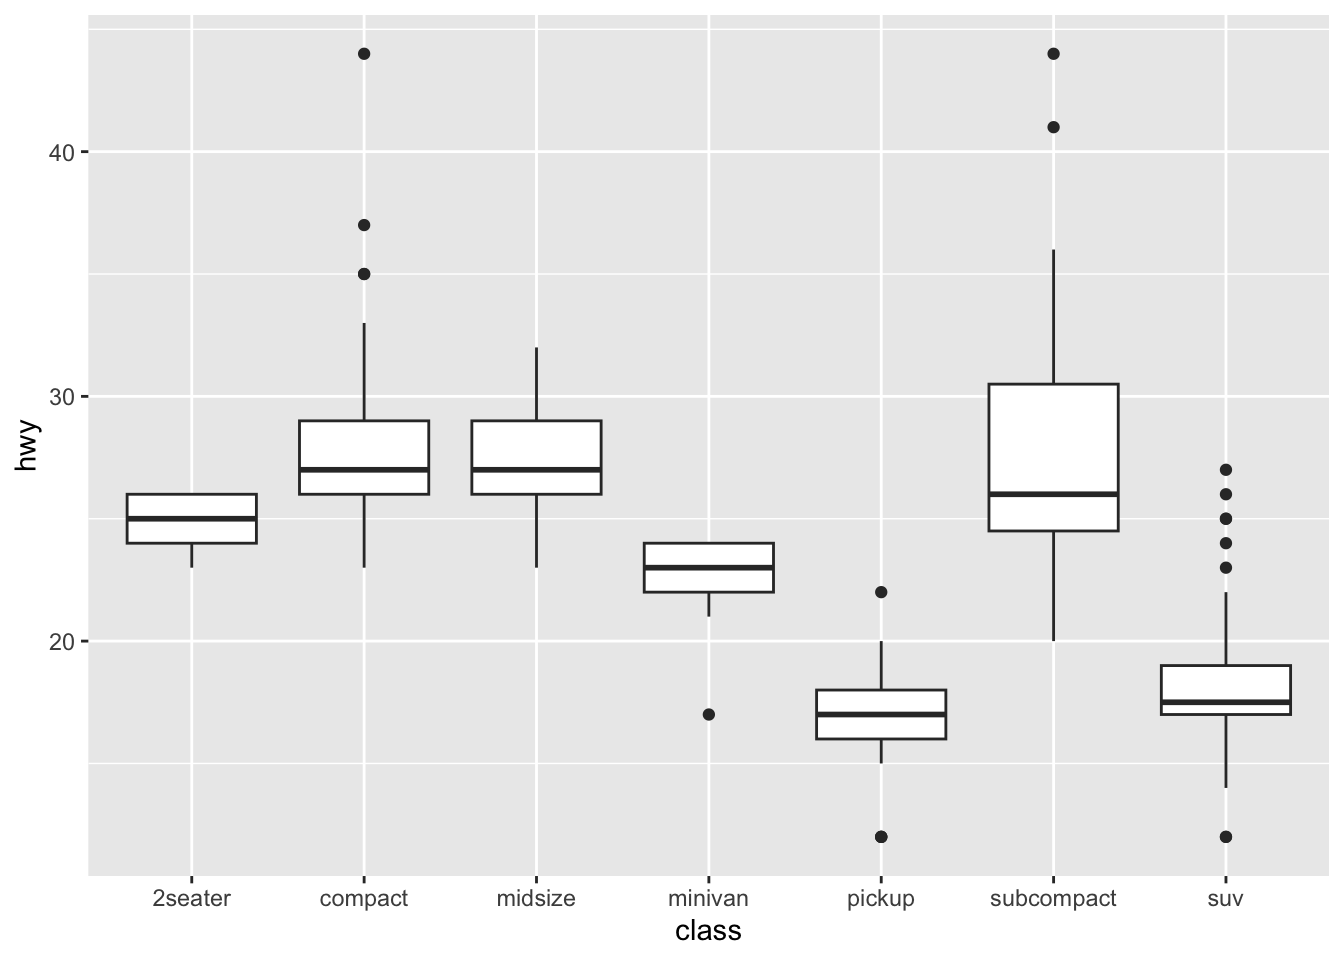
\includegraphics{08-Intermediate-R-II-Part1_files/figure-latex/unnamed-chunk-9-1.pdf}

\begin{itemize}
\tightlist
\item
  histogram
\end{itemize}

\begin{Shaded}
\begin{Highlighting}[]
\FunctionTok{ggplot}\NormalTok{(}\AttributeTok{data =}\NormalTok{ mpg) }\SpecialCharTok{+}
  \FunctionTok{geom\_histogram}\NormalTok{(}\AttributeTok{mapping =} \FunctionTok{aes}\NormalTok{(}\AttributeTok{x =}\NormalTok{ hwy))}
\CommentTok{\#\textgreater{} \textasciigrave{}stat\_bin()\textasciigrave{} using \textasciigrave{}bins = 30\textasciigrave{}. Pick better value with}
\CommentTok{\#\textgreater{} \textasciigrave{}binwidth\textasciigrave{}.}
\end{Highlighting}
\end{Shaded}

\includegraphics{08-Intermediate-R-II-Part1_files/figure-latex/unnamed-chunk-10-1.pdf}

\begin{Shaded}
\begin{Highlighting}[]
\FunctionTok{ggplot}\NormalTok{(}\AttributeTok{data =}\NormalTok{ mpg) }\SpecialCharTok{+}
  \FunctionTok{geom\_density}\NormalTok{(}\AttributeTok{mapping =} \FunctionTok{aes}\NormalTok{(}\AttributeTok{x =}\NormalTok{ hwy))}
\end{Highlighting}
\end{Shaded}

\includegraphics{08-Intermediate-R-II-Part1_files/figure-latex/unnamed-chunk-11-1.pdf}

Now you will add multiple geoms to the same plot.
Predict what the following code does:

\begin{Shaded}
\begin{Highlighting}[]
\FunctionTok{ggplot}\NormalTok{(}\AttributeTok{data =}\NormalTok{ mpg) }\SpecialCharTok{+}
  \FunctionTok{geom\_point}\NormalTok{(}\AttributeTok{mapping =} \FunctionTok{aes}\NormalTok{(}\AttributeTok{x =}\NormalTok{ displ, }\AttributeTok{y =}\NormalTok{ hwy)) }\SpecialCharTok{+}
  \FunctionTok{geom\_smooth}\NormalTok{(}\AttributeTok{mapping =} \FunctionTok{aes}\NormalTok{(}\AttributeTok{x =}\NormalTok{ displ, }\AttributeTok{y =}\NormalTok{ hwy))}
\CommentTok{\#\textgreater{} \textasciigrave{}geom\_smooth()\textasciigrave{} using method = \textquotesingle{}loess\textquotesingle{} and formula = \textquotesingle{}y \textasciitilde{}}
\CommentTok{\#\textgreater{} x\textquotesingle{}}
\end{Highlighting}
\end{Shaded}

\includegraphics{08-Intermediate-R-II-Part1_files/figure-latex/unnamed-chunk-12-1.pdf}

Mappings and data can be specified global (in \texttt{ggplot()}) or local.

\begin{Shaded}
\begin{Highlighting}[]
\FunctionTok{ggplot}\NormalTok{(}\AttributeTok{data =}\NormalTok{ mpg, }\AttributeTok{mapping =} \FunctionTok{aes}\NormalTok{(}\AttributeTok{x =}\NormalTok{ displ, }\AttributeTok{y =}\NormalTok{ hwy)) }\SpecialCharTok{+}
  \FunctionTok{geom\_point}\NormalTok{() }\SpecialCharTok{+}
  \FunctionTok{geom\_smooth}\NormalTok{() }\SpecialCharTok{+} \FunctionTok{theme\_bw}\NormalTok{()       }\CommentTok{\# adjust theme}
\CommentTok{\#\textgreater{} \textasciigrave{}geom\_smooth()\textasciigrave{} using method = \textquotesingle{}loess\textquotesingle{} and formula = \textquotesingle{}y \textasciitilde{}}
\CommentTok{\#\textgreater{} x\textquotesingle{}}
\end{Highlighting}
\end{Shaded}

\includegraphics{08-Intermediate-R-II-Part1_files/figure-latex/unnamed-chunk-13-1.pdf}

\textbf{local.}

\begin{Shaded}
\begin{Highlighting}[]
\FunctionTok{ggplot}\NormalTok{(}\AttributeTok{data =}\NormalTok{ mpg, }\AttributeTok{mapping =} \FunctionTok{aes}\NormalTok{(}\AttributeTok{x =}\NormalTok{ displ, }\AttributeTok{y =}\NormalTok{ hwy)) }\SpecialCharTok{+}
  \FunctionTok{geom\_point}\NormalTok{(}\AttributeTok{mapping =} \FunctionTok{aes}\NormalTok{(}\AttributeTok{color =}\NormalTok{ drv)) }\SpecialCharTok{+}
  \FunctionTok{geom\_smooth}\NormalTok{() }\SpecialCharTok{+} \FunctionTok{theme\_bw}\NormalTok{()}
\CommentTok{\#\textgreater{} \textasciigrave{}geom\_smooth()\textasciigrave{} using method = \textquotesingle{}loess\textquotesingle{} and formula = \textquotesingle{}y \textasciitilde{}}
\CommentTok{\#\textgreater{} x\textquotesingle{}}
\end{Highlighting}
\end{Shaded}

\includegraphics{08-Intermediate-R-II-Part1_files/figure-latex/unnamed-chunk-14-1.pdf}

\begin{Shaded}
\begin{Highlighting}[]
\FunctionTok{library}\NormalTok{(dplyr)}
\CommentTok{\#\textgreater{} }
\CommentTok{\#\textgreater{} Attaching package: \textquotesingle{}dplyr\textquotesingle{}}
\CommentTok{\#\textgreater{} The following objects are masked from \textquotesingle{}package:stats\textquotesingle{}:}
\CommentTok{\#\textgreater{} }
\CommentTok{\#\textgreater{}     filter, lag}
\CommentTok{\#\textgreater{} The following objects are masked from \textquotesingle{}package:base\textquotesingle{}:}
\CommentTok{\#\textgreater{} }
\CommentTok{\#\textgreater{}     intersect, setdiff, setequal, union}
\FunctionTok{ggplot}\NormalTok{(}\AttributeTok{data =}\NormalTok{ mpg, }\AttributeTok{mapping =} \FunctionTok{aes}\NormalTok{(}\AttributeTok{x =}\NormalTok{ displ, }\AttributeTok{y =}\NormalTok{ hwy)) }\SpecialCharTok{+}
  \FunctionTok{geom\_point}\NormalTok{(}\AttributeTok{mapping =} \FunctionTok{aes}\NormalTok{(}\AttributeTok{color =}\NormalTok{ drv)) }\SpecialCharTok{+}
  \FunctionTok{geom\_smooth}\NormalTok{(}\AttributeTok{data =} \FunctionTok{filter}\NormalTok{(mpg, drv }\SpecialCharTok{==} \StringTok{"f"}\NormalTok{)) }\SpecialCharTok{+} \FunctionTok{theme\_bw}\NormalTok{()}
\CommentTok{\#\textgreater{} \textasciigrave{}geom\_smooth()\textasciigrave{} using method = \textquotesingle{}loess\textquotesingle{} and formula = \textquotesingle{}y \textasciitilde{}}
\CommentTok{\#\textgreater{} x\textquotesingle{}}
\end{Highlighting}
\end{Shaded}

\includegraphics{08-Intermediate-R-II-Part1_files/figure-latex/unnamed-chunk-15-1.pdf}

\section*{Exercise 1}\label{exercise-1-6}
\addcontentsline{toc}{section}{Exercise 1}

Use the Danish fire insurance losses. Plot the arrival of losses over time.

\begin{enumerate}
\def\labelenumi{\arabic{enumi}.}
\tightlist
\item
  Use type= ``l'' for a line plot, label the and -axis, and give the plot a title using main.
\item
  Do the same with instructions from ggplot2. Use geom\_line() to create the line plot.
\end{enumerate}

\section*{Exercise 2}\label{exercise-2-5}
\addcontentsline{toc}{section}{Exercise 2}

\begin{enumerate}
\def\labelenumi{\arabic{enumi}.}
\item
  Use the data set car\_price.csv available in the documentation. Import the data in R.
\item
  Explore the data.
\item
  Make a scatterplot of price versus income, use basic plotting instructions
  and use ggplot2.
\item
  Add a smooth line to each of the plots (using lines to add a line to an existing plot and lowess to do scatterplot smoothing and using geom\_smooth in the ggplot2 grammar).
\end{enumerate}

\section*{Creating customized plots with ggplot2}\label{creating-customized-plots-with-ggplot2}
\addcontentsline{toc}{section}{Creating customized plots with ggplot2}

\begin{Shaded}
\begin{Highlighting}[]

\CommentTok{\# Load ggplot2 package}
\FunctionTok{library}\NormalTok{(ggplot2)}

\CommentTok{\# Example: Customized scatter plot with ggplot2}
\NormalTok{data }\OtherTok{\textless{}{-}} \FunctionTok{data.frame}\NormalTok{(}\AttributeTok{x =} \FunctionTok{rnorm}\NormalTok{(}\DecValTok{100}\NormalTok{), }\AttributeTok{y =} \FunctionTok{rnorm}\NormalTok{(}\DecValTok{100}\NormalTok{))}
\FunctionTok{ggplot}\NormalTok{(data, }\FunctionTok{aes}\NormalTok{(}\AttributeTok{x =}\NormalTok{ x, }\AttributeTok{y =}\NormalTok{ y)) }\SpecialCharTok{+}
  \FunctionTok{geom\_point}\NormalTok{(}\FunctionTok{aes}\NormalTok{(}\AttributeTok{color =}\NormalTok{ x}\SpecialCharTok{*}\NormalTok{y), }\AttributeTok{size =} \DecValTok{3}\NormalTok{) }\SpecialCharTok{+}
  \FunctionTok{scale\_color\_gradient}\NormalTok{(}\AttributeTok{low =} \StringTok{"blue"}\NormalTok{, }\AttributeTok{high =} \StringTok{"red"}\NormalTok{) }\SpecialCharTok{+}
  \FunctionTok{ggtitle}\NormalTok{(}\StringTok{"Customized Scatter Plot with Color Gradient"}\NormalTok{) }\SpecialCharTok{+}
  \FunctionTok{theme\_minimal}\NormalTok{()}
\end{Highlighting}
\end{Shaded}

\includegraphics{08-Intermediate-R-II-Part1_files/figure-latex/unnamed-chunk-16-1.pdf}

\section*{Adding titles, labels, and themes to plots}\label{adding-titles-labels-and-themes-to-plots}
\addcontentsline{toc}{section}{Adding titles, labels, and themes to plots}

\begin{Shaded}
\begin{Highlighting}[]
\CommentTok{\# Example: Enhanced bar plot with titles, labels, and a custom theme}
\NormalTok{data }\OtherTok{\textless{}{-}} \FunctionTok{data.frame}\NormalTok{(}
  \AttributeTok{category =} \FunctionTok{c}\NormalTok{(}\StringTok{"A"}\NormalTok{, }\StringTok{"B"}\NormalTok{, }\StringTok{"C"}\NormalTok{, }\StringTok{"D"}\NormalTok{),}
  \AttributeTok{value =} \FunctionTok{c}\NormalTok{(}\DecValTok{10}\NormalTok{, }\DecValTok{15}\NormalTok{, }\DecValTok{7}\NormalTok{, }\DecValTok{12}\NormalTok{)}
\NormalTok{)}
\FunctionTok{ggplot}\NormalTok{(data, }\FunctionTok{aes}\NormalTok{(}\AttributeTok{x =}\NormalTok{ category, }\AttributeTok{y =}\NormalTok{ value, }\AttributeTok{fill =}\NormalTok{ category)) }\SpecialCharTok{+}
  \FunctionTok{geom\_bar}\NormalTok{(}\AttributeTok{stat =} \StringTok{"identity"}\NormalTok{) }\SpecialCharTok{+}
  \FunctionTok{labs}\NormalTok{(}\AttributeTok{title =} \StringTok{"Enhanced Bar Plot"}\NormalTok{,}
       \AttributeTok{subtitle =} \StringTok{"Bar plot with custom labels and theme"}\NormalTok{,}
       \AttributeTok{x =} \StringTok{"Category"}\NormalTok{,}
       \AttributeTok{y =} \StringTok{"Value"}\NormalTok{,}
       \AttributeTok{fill =} \StringTok{"Category"}\NormalTok{) }\SpecialCharTok{+}
  \FunctionTok{theme\_bw}\NormalTok{() }\SpecialCharTok{+}
  \FunctionTok{theme}\NormalTok{(}\AttributeTok{plot.title =} \FunctionTok{element\_text}\NormalTok{(}\AttributeTok{hjust =} \FloatTok{0.5}\NormalTok{))}
\end{Highlighting}
\end{Shaded}

\includegraphics{08-Intermediate-R-II-Part1_files/figure-latex/unnamed-chunk-17-1.pdf}

\chapter*{Part IV: Statistical Analysis}\label{part-iv-statistical-analysis}
\addcontentsline{toc}{chapter}{Part IV: Statistical Analysis}

\section*{Introduction to hypothesis testing and statistical tests}\label{introduction-to-hypothesis-testing-and-statistical-tests}
\addcontentsline{toc}{section}{Introduction to hypothesis testing and statistical tests}

Hypothesis testing is a statistical method used to make inferences or draw conclusions about a population based on sample data. It starts with a null hypothesis (H0) that assumes no effect or no difference, and an alternative hypothesis (H1) that contradicts the null hypothesis.

The process involves:
1. Defining the null and alternative hypotheses.

\begin{enumerate}
\def\labelenumi{\arabic{enumi}.}
\setcounter{enumi}{1}
\item
  Selecting a significance level (alpha, typically 0.05).
\item
  Calculating a test statistic based on the sample data.
\item
  Determining the p-value, which is the probability of observing the test statistic or something more extreme under the null hypothesis.
\item
  Comparing the p-value with the significance level to decide whether to reject the null hypothesis.
\end{enumerate}

Statistical tests vary based on the type of data and the research question. Common tests include t-tests (for means), chi-squared tests (for categorical data), ANOVA (for comparing means across multiple groups), and regression analysis (for relationships between variables).

\section*{Comparing Variances}\label{comparing-variances}
\addcontentsline{toc}{section}{Comparing Variances}

\begin{enumerate}
\def\labelenumi{\alph{enumi}.}
\tightlist
\item
  F test to compare variances (Parametric)
\end{enumerate}

\begin{Shaded}
\begin{Highlighting}[]
\NormalTok{x }\OtherTok{\textless{}{-}} \FunctionTok{rnorm}\NormalTok{(}\DecValTok{50}\NormalTok{, }\AttributeTok{mean =} \DecValTok{0}\NormalTok{, }\AttributeTok{sd =} \DecValTok{2}\NormalTok{)}
\NormalTok{y }\OtherTok{\textless{}{-}} \FunctionTok{rnorm}\NormalTok{(}\DecValTok{30}\NormalTok{, }\AttributeTok{mean =} \DecValTok{1}\NormalTok{, }\AttributeTok{sd =} \DecValTok{1}\NormalTok{)}
\FunctionTok{var.test}\NormalTok{(x, y)}
\CommentTok{\#\textgreater{} }
\CommentTok{\#\textgreater{}  F test to compare two variances}
\CommentTok{\#\textgreater{} }
\CommentTok{\#\textgreater{} data:  x and y}
\CommentTok{\#\textgreater{} F = 7.0642, num df = 49, denom df = 29, p{-}value =}
\CommentTok{\#\textgreater{} 3.238e{-}07}
\CommentTok{\#\textgreater{} alternative hypothesis: true ratio of variances is not equal to 1}
\CommentTok{\#\textgreater{} 95 percent confidence interval:}
\CommentTok{\#\textgreater{}   3.549198 13.290630}
\CommentTok{\#\textgreater{} sample estimates:}
\CommentTok{\#\textgreater{} ratio of variances }
\CommentTok{\#\textgreater{}           7.064162}
\end{Highlighting}
\end{Shaded}

\begin{enumerate}
\def\labelenumi{\alph{enumi}.}
\setcounter{enumi}{1}
\tightlist
\item
  Barlett test: Testing homogeneity (Parametric)
\end{enumerate}

Performs Bartlett's test of the null that the variances in each of the groups (samples) are the same.

\begin{Shaded}
\begin{Highlighting}[]
\FunctionTok{require}\NormalTok{(graphics)}

\FunctionTok{plot}\NormalTok{(count }\SpecialCharTok{\textasciitilde{}}\NormalTok{ spray, }\AttributeTok{data =}\NormalTok{ InsectSprays)}
\end{Highlighting}
\end{Shaded}

\includegraphics{09-Intermediate-R-II-Part2_files/figure-latex/unnamed-chunk-2-1.pdf}

\begin{Shaded}
\begin{Highlighting}[]
\FunctionTok{bartlett.test}\NormalTok{(InsectSprays}\SpecialCharTok{$}\NormalTok{count, InsectSprays}\SpecialCharTok{$}\NormalTok{spray)}
\CommentTok{\#\textgreater{} }
\CommentTok{\#\textgreater{}  Bartlett test of homogeneity of variances}
\CommentTok{\#\textgreater{} }
\CommentTok{\#\textgreater{} data:  InsectSprays$count and InsectSprays$spray}
\CommentTok{\#\textgreater{} Bartlett\textquotesingle{}s K{-}squared = 25.96, df = 5, p{-}value =}
\CommentTok{\#\textgreater{} 9.085e{-}05}
\end{Highlighting}
\end{Shaded}

\begin{enumerate}
\def\labelenumi{\alph{enumi}.}
\setcounter{enumi}{2}
\tightlist
\item
  Fligner-Killeen Test of Homogeneity of Variances (Non-parametric)
\end{enumerate}

\begin{Shaded}
\begin{Highlighting}[]
\FunctionTok{fligner.test}\NormalTok{(InsectSprays}\SpecialCharTok{$}\NormalTok{count, InsectSprays}\SpecialCharTok{$}\NormalTok{spray)}
\CommentTok{\#\textgreater{} }
\CommentTok{\#\textgreater{}  Fligner{-}Killeen test of homogeneity of variances}
\CommentTok{\#\textgreater{} }
\CommentTok{\#\textgreater{} data:  InsectSprays$count and InsectSprays$spray}
\CommentTok{\#\textgreater{} Fligner{-}Killeen:med chi{-}squared = 14.483, df = 5,}
\CommentTok{\#\textgreater{} p{-}value = 0.01282}
\end{Highlighting}
\end{Shaded}

\begin{enumerate}
\def\labelenumi{\alph{enumi}.}
\setcounter{enumi}{3}
\tightlist
\item
  Mood Two-Sample Test of Scale (Non-Parametric)
\end{enumerate}

\begin{Shaded}
\begin{Highlighting}[]
\NormalTok{ramsay }\OtherTok{\textless{}{-}} \FunctionTok{c}\NormalTok{(}\DecValTok{111}\NormalTok{, }\DecValTok{107}\NormalTok{, }\DecValTok{100}\NormalTok{, }\DecValTok{99}\NormalTok{, }\DecValTok{102}\NormalTok{, }\DecValTok{106}\NormalTok{, }\DecValTok{109}\NormalTok{, }\DecValTok{108}\NormalTok{, }\DecValTok{104}\NormalTok{, }\DecValTok{99}\NormalTok{,}
            \DecValTok{101}\NormalTok{, }\DecValTok{96}\NormalTok{, }\DecValTok{97}\NormalTok{, }\DecValTok{102}\NormalTok{, }\DecValTok{107}\NormalTok{, }\DecValTok{113}\NormalTok{, }\DecValTok{116}\NormalTok{, }\DecValTok{113}\NormalTok{, }\DecValTok{110}\NormalTok{, }\DecValTok{98}\NormalTok{)}
\NormalTok{jung.parekh }\OtherTok{\textless{}{-}} \FunctionTok{c}\NormalTok{(}\DecValTok{107}\NormalTok{, }\DecValTok{108}\NormalTok{, }\DecValTok{106}\NormalTok{, }\DecValTok{98}\NormalTok{, }\DecValTok{105}\NormalTok{, }\DecValTok{103}\NormalTok{, }\DecValTok{110}\NormalTok{, }\DecValTok{105}\NormalTok{, }\DecValTok{104}\NormalTok{,}
            \DecValTok{100}\NormalTok{, }\DecValTok{96}\NormalTok{, }\DecValTok{108}\NormalTok{, }\DecValTok{103}\NormalTok{, }\DecValTok{104}\NormalTok{, }\DecValTok{114}\NormalTok{, }\DecValTok{114}\NormalTok{, }\DecValTok{113}\NormalTok{, }\DecValTok{108}\NormalTok{, }\DecValTok{106}\NormalTok{, }\DecValTok{99}\NormalTok{)}
\FunctionTok{mood.test}\NormalTok{(ramsay, jung.parekh)}
\CommentTok{\#\textgreater{} }
\CommentTok{\#\textgreater{}  Mood two{-}sample test of scale}
\CommentTok{\#\textgreater{} }
\CommentTok{\#\textgreater{} data:  ramsay and jung.parekh}
\CommentTok{\#\textgreater{} Z = 1.0371, p{-}value = 0.2997}
\CommentTok{\#\textgreater{} alternative hypothesis: two.sided}
\end{Highlighting}
\end{Shaded}

\begin{enumerate}
\def\labelenumi{\alph{enumi}.}
\setcounter{enumi}{4}
\tightlist
\item
  Ansari-Bradley Test (Non-parametric)
\end{enumerate}

\begin{Shaded}
\begin{Highlighting}[]
\NormalTok{ramsay }\OtherTok{\textless{}{-}} \FunctionTok{c}\NormalTok{(}\DecValTok{111}\NormalTok{, }\DecValTok{107}\NormalTok{, }\DecValTok{100}\NormalTok{, }\DecValTok{99}\NormalTok{, }\DecValTok{102}\NormalTok{, }\DecValTok{106}\NormalTok{, }\DecValTok{109}\NormalTok{, }\DecValTok{108}\NormalTok{, }\DecValTok{104}\NormalTok{, }\DecValTok{99}\NormalTok{,}
            \DecValTok{101}\NormalTok{, }\DecValTok{96}\NormalTok{, }\DecValTok{97}\NormalTok{, }\DecValTok{102}\NormalTok{, }\DecValTok{107}\NormalTok{, }\DecValTok{113}\NormalTok{, }\DecValTok{116}\NormalTok{, }\DecValTok{113}\NormalTok{, }\DecValTok{110}\NormalTok{, }\DecValTok{98}\NormalTok{)}
\NormalTok{jung.parekh }\OtherTok{\textless{}{-}} \FunctionTok{c}\NormalTok{(}\DecValTok{107}\NormalTok{, }\DecValTok{108}\NormalTok{, }\DecValTok{106}\NormalTok{, }\DecValTok{98}\NormalTok{, }\DecValTok{105}\NormalTok{, }\DecValTok{103}\NormalTok{, }\DecValTok{110}\NormalTok{, }\DecValTok{105}\NormalTok{, }\DecValTok{104}\NormalTok{,}
            \DecValTok{100}\NormalTok{, }\DecValTok{96}\NormalTok{, }\DecValTok{108}\NormalTok{, }\DecValTok{103}\NormalTok{, }\DecValTok{104}\NormalTok{, }\DecValTok{114}\NormalTok{, }\DecValTok{114}\NormalTok{, }\DecValTok{113}\NormalTok{, }\DecValTok{108}\NormalTok{, }\DecValTok{106}\NormalTok{, }\DecValTok{99}\NormalTok{)}
\FunctionTok{ansari.test}\NormalTok{(ramsay, jung.parekh)}
\CommentTok{\#\textgreater{} Warning in ansari.test.default(ramsay, jung.parekh): cannot}
\CommentTok{\#\textgreater{} compute exact p{-}value with ties}
\CommentTok{\#\textgreater{} }
\CommentTok{\#\textgreater{}  Ansari{-}Bradley test}
\CommentTok{\#\textgreater{} }
\CommentTok{\#\textgreater{} data:  ramsay and jung.parekh}
\CommentTok{\#\textgreater{} AB = 185.5, p{-}value = 0.1815}
\CommentTok{\#\textgreater{} alternative hypothesis: true ratio of scales is not equal to 1}
\end{Highlighting}
\end{Shaded}

Testing two normal distributions

\begin{Shaded}
\begin{Highlighting}[]
\FunctionTok{ansari.test}\NormalTok{(}\FunctionTok{rnorm}\NormalTok{(}\DecValTok{100}\NormalTok{), }\FunctionTok{rnorm}\NormalTok{(}\DecValTok{100}\NormalTok{, }\DecValTok{0}\NormalTok{, }\DecValTok{2}\NormalTok{), }\AttributeTok{conf.int =} \ConstantTok{TRUE}\NormalTok{)}
\CommentTok{\#\textgreater{} }
\CommentTok{\#\textgreater{}  Ansari{-}Bradley test}
\CommentTok{\#\textgreater{} }
\CommentTok{\#\textgreater{} data:  rnorm(100) and rnorm(100, 0, 2)}
\CommentTok{\#\textgreater{} AB = 6202, p{-}value = 1.804e{-}08}
\CommentTok{\#\textgreater{} alternative hypothesis: true ratio of scales is not equal to 1}
\CommentTok{\#\textgreater{} 95 percent confidence interval:}
\CommentTok{\#\textgreater{}  0.3570530 0.5994205}
\CommentTok{\#\textgreater{} sample estimates:}
\CommentTok{\#\textgreater{} ratio of scales }
\CommentTok{\#\textgreater{}       0.4689279}
\end{Highlighting}
\end{Shaded}

\section*{Performing Tests}\label{performing-tests}
\addcontentsline{toc}{section}{Performing Tests}

\begin{enumerate}
\def\labelenumi{\arabic{enumi}.}
\tightlist
\item
  Tests for Comparing Means
\end{enumerate}

\begin{enumerate}
\def\labelenumi{\alph{enumi}.}
\tightlist
\item
  One-Sample t-Test
\end{enumerate}

We'll test if the average miles per gallon (mpg) in the mtcars dataset is significantly different from 20 mpg.

\begin{Shaded}
\begin{Highlighting}[]
\FunctionTok{t.test}\NormalTok{(mtcars}\SpecialCharTok{$}\NormalTok{mpg, }\AttributeTok{mu =} \DecValTok{20}\NormalTok{)}
\CommentTok{\#\textgreater{} }
\CommentTok{\#\textgreater{}  One Sample t{-}test}
\CommentTok{\#\textgreater{} }
\CommentTok{\#\textgreater{} data:  mtcars$mpg}
\CommentTok{\#\textgreater{} t = 0.08506, df = 31, p{-}value = 0.9328}
\CommentTok{\#\textgreater{} alternative hypothesis: true mean is not equal to 20}
\CommentTok{\#\textgreater{} 95 percent confidence interval:}
\CommentTok{\#\textgreater{}  17.91768 22.26357}
\CommentTok{\#\textgreater{} sample estimates:}
\CommentTok{\#\textgreater{} mean of x }
\CommentTok{\#\textgreater{}  20.09062}
\end{Highlighting}
\end{Shaded}

The results of this one-sample t-test suggest that the average mpg for the cars in the \texttt{mtcars} dataset is not significantly different from 20 mpg, as the p-value is far above the typical alpha level of 0.05 used to determine statistical significance. The data supports the null hypothesis that the true mean is 20 mpg, within the confidence interval provided.

\begin{enumerate}
\def\labelenumi{\alph{enumi}.}
\setcounter{enumi}{1}
\tightlist
\item
  Independent Two-Sample t-Test
\end{enumerate}

We'll compare the means of mpg between cars with automatic (am = 0) and manual (am = 1) transmissions.

\begin{Shaded}
\begin{Highlighting}[]
\NormalTok{auto\_mpg }\OtherTok{\textless{}{-}}\NormalTok{ mtcars}\SpecialCharTok{$}\NormalTok{mpg[mtcars}\SpecialCharTok{$}\NormalTok{am }\SpecialCharTok{==} \DecValTok{0}\NormalTok{]}
\NormalTok{manual\_mpg }\OtherTok{\textless{}{-}}\NormalTok{ mtcars}\SpecialCharTok{$}\NormalTok{mpg[mtcars}\SpecialCharTok{$}\NormalTok{am }\SpecialCharTok{==} \DecValTok{1}\NormalTok{]}
\FunctionTok{t.test}\NormalTok{(auto\_mpg, manual\_mpg, }\AttributeTok{var.equal =} \ConstantTok{TRUE}\NormalTok{)}
\CommentTok{\#\textgreater{} }
\CommentTok{\#\textgreater{}  Two Sample t{-}test}
\CommentTok{\#\textgreater{} }
\CommentTok{\#\textgreater{} data:  auto\_mpg and manual\_mpg}
\CommentTok{\#\textgreater{} t = {-}4.1061, df = 30, p{-}value = 0.000285}
\CommentTok{\#\textgreater{} alternative hypothesis: true difference in means is not equal to 0}
\CommentTok{\#\textgreater{} 95 percent confidence interval:}
\CommentTok{\#\textgreater{}  {-}10.84837  {-}3.64151}
\CommentTok{\#\textgreater{} sample estimates:}
\CommentTok{\#\textgreater{} mean of x mean of y }
\CommentTok{\#\textgreater{}  17.14737  24.39231}
\end{Highlighting}
\end{Shaded}

The results of this two-sample t-test indicate that the average mpg for cars with automatic transmissions significantly differs from those with manual transmissions, as the p-value (0.000285) is well below the alpha level of 0.05 typically used for determining statistical significance. The data strongly support the alternative hypothesis that there is a true difference in means, with manual transmission cars averaging higher mpg (24.39 mpg) compared to automatics (17.15 mpg), as reflected within the confidence interval provided.

\begin{enumerate}
\def\labelenumi{\alph{enumi}.}
\setcounter{enumi}{2}
\tightlist
\item
  Paired t-Test
\end{enumerate}

Let's use sleep data

\begin{Shaded}
\begin{Highlighting}[]
\CommentTok{\# Load the dataset}
\FunctionTok{data}\NormalTok{(sleep)}

\CommentTok{\# Perform the paired t{-}test comparing the effects of two drugs}
\NormalTok{t\_test\_result }\OtherTok{\textless{}{-}} \FunctionTok{t.test}\NormalTok{(extra }\SpecialCharTok{\textasciitilde{}}\NormalTok{ group, }\AttributeTok{data =}\NormalTok{ sleep, }\AttributeTok{paired =} \ConstantTok{TRUE}\NormalTok{)}

\CommentTok{\# Print the results}
\FunctionTok{print}\NormalTok{(t\_test\_result)}
\CommentTok{\#\textgreater{} }
\CommentTok{\#\textgreater{}  Paired t{-}test}
\CommentTok{\#\textgreater{} }
\CommentTok{\#\textgreater{} data:  extra by group}
\CommentTok{\#\textgreater{} t = {-}4.0621, df = 9, p{-}value = 0.002833}
\CommentTok{\#\textgreater{} alternative hypothesis: true mean difference is not equal to 0}
\CommentTok{\#\textgreater{} 95 percent confidence interval:}
\CommentTok{\#\textgreater{}  {-}2.4598858 {-}0.7001142}
\CommentTok{\#\textgreater{} sample estimates:}
\CommentTok{\#\textgreater{} mean difference }
\CommentTok{\#\textgreater{}           {-}1.58}
\end{Highlighting}
\end{Shaded}

The results of this paired t-test suggest that there is a statistically significant difference in the \texttt{extra} sleep effects between the two treatment groups, as the p-value (0.002833) is well below the typical alpha level of 0.05 used for determining statistical significance. The data strongly support the alternative hypothesis that the true mean difference in sleep effects is not equal to zero, with an average mean difference of -1.58 hours. This difference indicates that one treatment group experienced a greater increase in sleep duration compared to the other, as confirmed by the confidence interval ranging from -2.46 to -0.70 hours.

\begin{enumerate}
\def\labelenumi{\alph{enumi}.}
\setcounter{enumi}{3}
\tightlist
\item
  One-Way ANOVA
\end{enumerate}

Test if there are differences in mpg across different levels of the number of cylinders (cyl).

\begin{Shaded}
\begin{Highlighting}[]
\NormalTok{anova\_model }\OtherTok{\textless{}{-}} \FunctionTok{aov}\NormalTok{(mpg }\SpecialCharTok{\textasciitilde{}} \FunctionTok{factor}\NormalTok{(cyl), }\AttributeTok{data =}\NormalTok{ mtcars)}
\FunctionTok{summary}\NormalTok{(anova\_model)}
\CommentTok{\#\textgreater{}             Df Sum Sq Mean Sq F value   Pr(\textgreater{}F)    }
\CommentTok{\#\textgreater{} factor(cyl)  2  824.8   412.4    39.7 4.98e{-}09 ***}
\CommentTok{\#\textgreater{} Residuals   29  301.3    10.4                     }
\CommentTok{\#\textgreater{} {-}{-}{-}}
\CommentTok{\#\textgreater{} Signif. codes:  }
\CommentTok{\#\textgreater{} 0 \textquotesingle{}***\textquotesingle{} 0.001 \textquotesingle{}**\textquotesingle{} 0.01 \textquotesingle{}*\textquotesingle{} 0.05 \textquotesingle{}.\textquotesingle{} 0.1 \textquotesingle{} \textquotesingle{} 1}
\end{Highlighting}
\end{Shaded}

The ANOVA analysis clearly shows that the number of cylinders in a vehicle significantly affects its fuel efficiency, with different cylinder groups exhibiting notably different mpg. This finding is robust, with very strong statistical significance, suggesting that engine size, as indicated by the number of cylinders, is a key factor influencing a car's fuel consumption. This information can be vital for both consumers seeking fuel-efficient vehicles and manufacturers aiming to improve vehicle designs.

\begin{enumerate}
\def\labelenumi{\alph{enumi}.}
\setcounter{enumi}{4}
\tightlist
\item
  Repeated Measures ANOVA
\end{enumerate}

\begin{Shaded}
\begin{Highlighting}[]
\CommentTok{\# Load the CO2 dataset from the datasets package}
\FunctionTok{data}\NormalTok{(CO2)}

\CommentTok{\# Check the structure of the data}
\FunctionTok{str}\NormalTok{(CO2)}
\CommentTok{\#\textgreater{} Classes \textquotesingle{}nfnGroupedData\textquotesingle{}, \textquotesingle{}nfGroupedData\textquotesingle{}, \textquotesingle{}groupedData\textquotesingle{} and \textquotesingle{}data.frame\textquotesingle{}:   84 obs. of  5 variables:}
\CommentTok{\#\textgreater{}  $ Plant    : Ord.factor w/ 12 levels "Qn1"\textless{}"Qn2"\textless{}"Qn3"\textless{}..: 1 1 1 1 1 1 1 2 2 2 ...}
\CommentTok{\#\textgreater{}  $ Type     : Factor w/ 2 levels "Quebec","Mississippi": 1 1 1 1 1 1 1 1 1 1 ...}
\CommentTok{\#\textgreater{}  $ Treatment: Factor w/ 2 levels "nonchilled","chilled": 1 1 1 1 1 1 1 1 1 1 ...}
\CommentTok{\#\textgreater{}  $ conc     : num  95 175 250 350 500 675 1000 95 175 250 ...}
\CommentTok{\#\textgreater{}  $ uptake   : num  16 30.4 34.8 37.2 35.3 39.2 39.7 13.6 27.3 37.1 ...}
\CommentTok{\#\textgreater{}  {-} attr(*, "formula")=Class \textquotesingle{}formula\textquotesingle{}  language uptake \textasciitilde{} conc | Plant}
\CommentTok{\#\textgreater{}   .. ..{-} attr(*, ".Environment")=\textless{}environment: R\_EmptyEnv\textgreater{} }
\CommentTok{\#\textgreater{}  {-} attr(*, "outer")=Class \textquotesingle{}formula\textquotesingle{}  language \textasciitilde{}Treatment * Type}
\CommentTok{\#\textgreater{}   .. ..{-} attr(*, ".Environment")=\textless{}environment: R\_EmptyEnv\textgreater{} }
\CommentTok{\#\textgreater{}  {-} attr(*, "labels")=List of 2}
\CommentTok{\#\textgreater{}   ..$ x: chr "Ambient carbon dioxide concentration"}
\CommentTok{\#\textgreater{}   ..$ y: chr "CO2 uptake rate"}
\CommentTok{\#\textgreater{}  {-} attr(*, "units")=List of 2}
\CommentTok{\#\textgreater{}   ..$ x: chr "(uL/L)"}
\CommentTok{\#\textgreater{}   ..$ y: chr "(umol/m\^{}2 s)"}

\CommentTok{\# Load necessary package for analysis}
\CommentTok{\#install.packages("nlme") }
\FunctionTok{library}\NormalTok{(nlme)  }\CommentTok{\# for linear mixed{-}effects models}

\CommentTok{\# Fit a repeated measures model}
\CommentTok{\# Treat \textquotesingle{}Plant\textquotesingle{} as a random effect to account for measurements from the same plant}
\NormalTok{model }\OtherTok{\textless{}{-}} \FunctionTok{lme}\NormalTok{(uptake }\SpecialCharTok{\textasciitilde{}}\NormalTok{ Type }\SpecialCharTok{*}\NormalTok{ Treatment, }\AttributeTok{random =} \SpecialCharTok{\textasciitilde{}} \DecValTok{1} \SpecialCharTok{|}\NormalTok{ Plant, }\AttributeTok{data =}\NormalTok{ CO2)}

\CommentTok{\# Summary of the model}
\FunctionTok{summary}\NormalTok{(model)}
\CommentTok{\#\textgreater{} Linear mixed{-}effects model fit by REML}
\CommentTok{\#\textgreater{}   Data: CO2 }
\CommentTok{\#\textgreater{}        AIC      BIC    logLik}
\CommentTok{\#\textgreater{}   584.0375 598.3297 {-}286.0188}
\CommentTok{\#\textgreater{} }
\CommentTok{\#\textgreater{} Random effects:}
\CommentTok{\#\textgreater{}  Formula: \textasciitilde{}1 | Plant}
\CommentTok{\#\textgreater{}          (Intercept) Residual}
\CommentTok{\#\textgreater{} StdDev: 0.0004510923 8.005933}
\CommentTok{\#\textgreater{} }
\CommentTok{\#\textgreater{} Fixed effects:  uptake \textasciitilde{} Type * Treatment }
\CommentTok{\#\textgreater{}                                     Value Std.Error DF}
\CommentTok{\#\textgreater{} (Intercept)                      35.33333  1.747038 72}
\CommentTok{\#\textgreater{} TypeMississippi                  {-}9.38095  2.470685  8}
\CommentTok{\#\textgreater{} Treatmentchilled                 {-}3.58095  2.470685  8}
\CommentTok{\#\textgreater{} TypeMississippi:Treatmentchilled {-}6.55714  3.494076  8}
\CommentTok{\#\textgreater{}                                    t{-}value p{-}value}
\CommentTok{\#\textgreater{} (Intercept)                      20.224710  0.0000}
\CommentTok{\#\textgreater{} TypeMississippi                  {-}3.796904  0.0053}
\CommentTok{\#\textgreater{} Treatmentchilled                 {-}1.449377  0.1853}
\CommentTok{\#\textgreater{} TypeMississippi:Treatmentchilled {-}1.876646  0.0974}
\CommentTok{\#\textgreater{}  Correlation: }
\CommentTok{\#\textgreater{}                                  (Intr) TypMss Trtmnt}
\CommentTok{\#\textgreater{} TypeMississippi                  {-}0.707              }
\CommentTok{\#\textgreater{} Treatmentchilled                 {-}0.707  0.500       }
\CommentTok{\#\textgreater{} TypeMississippi:Treatmentchilled  0.500 {-}0.707 {-}0.707}
\CommentTok{\#\textgreater{} }
\CommentTok{\#\textgreater{} Standardized Within{-}Group Residuals:}
\CommentTok{\#\textgreater{}        Min         Q1        Med         Q3        Max }
\CommentTok{\#\textgreater{} {-}2.8044677 {-}0.4526405  0.2706326  0.7210426  1.3299660 }
\CommentTok{\#\textgreater{} }
\CommentTok{\#\textgreater{} Number of Observations: 84}
\CommentTok{\#\textgreater{} Number of Groups: 12}

\CommentTok{\# Anova table for the model}
\FunctionTok{anova}\NormalTok{(model)}
\CommentTok{\#\textgreater{}                numDF denDF  F{-}value p{-}value}
\CommentTok{\#\textgreater{} (Intercept)        1    72 970.5351  \textless{}.0001}
\CommentTok{\#\textgreater{} Type               1     8  52.5086  0.0001}
\CommentTok{\#\textgreater{} Treatment          1     8  15.4164  0.0044}
\CommentTok{\#\textgreater{} Type:Treatment     1     8   3.5218  0.0974}
\end{Highlighting}
\end{Shaded}

The model provides strong evidence that both the type of plant and whether it is chilled significantly affect CO2 uptake, independently. The lack of a significant interaction suggests that the effect of chilling does not differ between types in the way that might have been expected.

\begin{enumerate}
\def\labelenumi{\arabic{enumi}.}
\setcounter{enumi}{1}
\tightlist
\item
  Tests for Comparing Medians
\end{enumerate}

\begin{enumerate}
\def\labelenumi{\alph{enumi}.}
\tightlist
\item
  Mann-Whitney U Test
\end{enumerate}

Comparing mpg between cars with 4 and 6 cylinders.

\begin{Shaded}
\begin{Highlighting}[]
\NormalTok{mpg\_4 }\OtherTok{\textless{}{-}}\NormalTok{ mtcars}\SpecialCharTok{$}\NormalTok{mpg[mtcars}\SpecialCharTok{$}\NormalTok{cyl }\SpecialCharTok{==} \DecValTok{4}\NormalTok{]}
\NormalTok{mpg\_6 }\OtherTok{\textless{}{-}}\NormalTok{ mtcars}\SpecialCharTok{$}\NormalTok{mpg[mtcars}\SpecialCharTok{$}\NormalTok{cyl }\SpecialCharTok{==} \DecValTok{6}\NormalTok{]}
\FunctionTok{wilcox.test}\NormalTok{(mpg\_4, mpg\_6)}
\CommentTok{\#\textgreater{} Warning in wilcox.test.default(mpg\_4, mpg\_6): cannot}
\CommentTok{\#\textgreater{} compute exact p{-}value with ties}
\CommentTok{\#\textgreater{} }
\CommentTok{\#\textgreater{}  Wilcoxon rank sum test with continuity correction}
\CommentTok{\#\textgreater{} }
\CommentTok{\#\textgreater{} data:  mpg\_4 and mpg\_6}
\CommentTok{\#\textgreater{} W = 76.5, p{-}value = 0.0006658}
\CommentTok{\#\textgreater{} alternative hypothesis: true location shift is not equal to 0}
\end{Highlighting}
\end{Shaded}

The result of the Wilcoxon rank sum test strongly suggests that the median mpg values for cars with 4 cylinders differ significantly from those with 6 cylinders in the mtcars dataset. Given the very low p-value, it is likely that 4-cylinder cars either achieve higher or lower mpg compared to 6-cylinder cars, depending on the direction of the rank sums (not specified here but typically inferred from the data setup). This finding is crucial for automotive studies focusing on fuel efficiency based on engine size, providing evidence that engine size (as represented by cylinder count) may impact fuel economy.

\begin{enumerate}
\def\labelenumi{\alph{enumi}.}
\setcounter{enumi}{1}
\tightlist
\item
  Wilcoxon Signed-Rank Test
\end{enumerate}

Again, a hypothetical example for paired data.

\begin{Shaded}
\begin{Highlighting}[]

\CommentTok{\# Extracting the groups}

\NormalTok{group1 }\OtherTok{\textless{}{-}}\NormalTok{ sleep}\SpecialCharTok{$}\NormalTok{extra[sleep}\SpecialCharTok{$}\NormalTok{group }\SpecialCharTok{==} \DecValTok{1}\NormalTok{]}
\NormalTok{group2 }\OtherTok{\textless{}{-}}\NormalTok{ sleep}\SpecialCharTok{$}\NormalTok{extra[sleep}\SpecialCharTok{$}\NormalTok{group }\SpecialCharTok{==} \DecValTok{2}\NormalTok{]}

\CommentTok{\# Wilcoxon Signed{-}Rank Test}
\NormalTok{wilcox\_test\_results }\OtherTok{\textless{}{-}} \FunctionTok{wilcox.test}\NormalTok{(group1, group2, }\AttributeTok{paired =} \ConstantTok{TRUE}\NormalTok{)}
\CommentTok{\#\textgreater{} Warning in wilcox.test.default(group1, group2, paired =}
\CommentTok{\#\textgreater{} TRUE): cannot compute exact p{-}value with ties}
\CommentTok{\#\textgreater{} Warning in wilcox.test.default(group1, group2, paired =}
\CommentTok{\#\textgreater{} TRUE): cannot compute exact p{-}value with zeroes}

\CommentTok{\# Print the results}
\FunctionTok{print}\NormalTok{(wilcox\_test\_results)}
\CommentTok{\#\textgreater{} }
\CommentTok{\#\textgreater{}  Wilcoxon signed rank test with continuity correction}
\CommentTok{\#\textgreater{} }
\CommentTok{\#\textgreater{} data:  group1 and group2}
\CommentTok{\#\textgreater{} V = 0, p{-}value = 0.009091}
\CommentTok{\#\textgreater{} alternative hypothesis: true location shift is not equal to 0}
\end{Highlighting}
\end{Shaded}

The results of the Wilcoxon signed-rank test suggest a statistically significant difference between the two groups tested, with a p-value indicating strong evidence against the null hypothesis of no difference. This significant finding implies that the treatment or condition represented by these two groups had a different impact on the variable measured (extra sleep hours), with the direction of effect (which group had more sleep) needing further description from the data setup. This analysis is particularly useful in clinical or psychological studies where the normality assumption may not hold, and robust, non-parametric methods are required.

\begin{Shaded}
\begin{Highlighting}[]
\NormalTok{x }\OtherTok{\textless{}{-}} \FunctionTok{c}\NormalTok{(}\FloatTok{1.83}\NormalTok{,  }\FloatTok{0.50}\NormalTok{,  }\FloatTok{1.62}\NormalTok{,  }\FloatTok{2.48}\NormalTok{, }\FloatTok{1.68}\NormalTok{, }\FloatTok{1.88}\NormalTok{, }\FloatTok{1.55}\NormalTok{, }\FloatTok{3.06}\NormalTok{, }\FloatTok{1.30}\NormalTok{)}
\NormalTok{y }\OtherTok{\textless{}{-}} \FunctionTok{c}\NormalTok{(}\FloatTok{0.878}\NormalTok{, }\FloatTok{0.647}\NormalTok{, }\FloatTok{0.598}\NormalTok{, }\FloatTok{2.05}\NormalTok{, }\FloatTok{1.06}\NormalTok{, }\FloatTok{1.29}\NormalTok{, }\FloatTok{1.06}\NormalTok{, }\FloatTok{3.14}\NormalTok{, }\FloatTok{1.29}\NormalTok{)}
\FunctionTok{wilcox.test}\NormalTok{(x, y, }\AttributeTok{paired =} \ConstantTok{TRUE}\NormalTok{, }\AttributeTok{alternative =} \StringTok{"greater"}\NormalTok{)}
\CommentTok{\#\textgreater{} }
\CommentTok{\#\textgreater{}  Wilcoxon signed rank exact test}
\CommentTok{\#\textgreater{} }
\CommentTok{\#\textgreater{} data:  x and y}
\CommentTok{\#\textgreater{} V = 40, p{-}value = 0.01953}
\CommentTok{\#\textgreater{} alternative hypothesis: true location shift is greater than 0}
\end{Highlighting}
\end{Shaded}

\begin{enumerate}
\def\labelenumi{\alph{enumi}.}
\setcounter{enumi}{2}
\tightlist
\item
  Kruskal-Wallis Test
\end{enumerate}

Comparing mpg across different cylinder groups.

\begin{Shaded}
\begin{Highlighting}[]
\FunctionTok{kruskal.test}\NormalTok{(mpg }\SpecialCharTok{\textasciitilde{}} \FunctionTok{factor}\NormalTok{(cyl), }\AttributeTok{data =}\NormalTok{ mtcars)}
\CommentTok{\#\textgreater{} }
\CommentTok{\#\textgreater{}  Kruskal{-}Wallis rank sum test}
\CommentTok{\#\textgreater{} }
\CommentTok{\#\textgreater{} data:  mpg by factor(cyl)}
\CommentTok{\#\textgreater{} Kruskal{-}Wallis chi{-}squared = 25.746, df = 2, p{-}value}
\CommentTok{\#\textgreater{} = 2.566e{-}06}
\end{Highlighting}
\end{Shaded}

The Kruskal-Wallis test conclusively shows that the number of cylinders is a significant factor in determining a car's miles per gallon, with the differences in mpg across groups being statistically significant. This insight can inform decisions related to car manufacturing and consumer choice, particularly in contexts where fuel efficiency is a critical concern.

\begin{enumerate}
\def\labelenumi{\alph{enumi}.}
\setcounter{enumi}{3}
\tightlist
\item
  Friedman Test
\end{enumerate}

\begin{Shaded}
\begin{Highlighting}[]
\NormalTok{RoundingTimes }\OtherTok{\textless{}{-}}
\FunctionTok{matrix}\NormalTok{(}\FunctionTok{c}\NormalTok{(}\FloatTok{5.40}\NormalTok{, }\FloatTok{5.50}\NormalTok{, }\FloatTok{5.55}\NormalTok{,}
         \FloatTok{5.85}\NormalTok{, }\FloatTok{5.70}\NormalTok{, }\FloatTok{5.75}\NormalTok{,}
         \FloatTok{5.20}\NormalTok{, }\FloatTok{5.60}\NormalTok{, }\FloatTok{5.50}\NormalTok{,}
         \FloatTok{5.55}\NormalTok{, }\FloatTok{5.50}\NormalTok{, }\FloatTok{5.40}\NormalTok{,}
         \FloatTok{5.90}\NormalTok{, }\FloatTok{5.85}\NormalTok{, }\FloatTok{5.70}\NormalTok{,}
         \FloatTok{5.45}\NormalTok{, }\FloatTok{5.55}\NormalTok{, }\FloatTok{5.60}\NormalTok{,}
         \FloatTok{5.40}\NormalTok{, }\FloatTok{5.40}\NormalTok{, }\FloatTok{5.35}\NormalTok{,}
         \FloatTok{5.45}\NormalTok{, }\FloatTok{5.50}\NormalTok{, }\FloatTok{5.35}\NormalTok{,}
         \FloatTok{5.25}\NormalTok{, }\FloatTok{5.15}\NormalTok{, }\FloatTok{5.00}\NormalTok{,}
         \FloatTok{5.85}\NormalTok{, }\FloatTok{5.80}\NormalTok{, }\FloatTok{5.70}\NormalTok{,}
         \FloatTok{5.25}\NormalTok{, }\FloatTok{5.20}\NormalTok{, }\FloatTok{5.10}\NormalTok{,}
         \FloatTok{5.65}\NormalTok{, }\FloatTok{5.55}\NormalTok{, }\FloatTok{5.45}\NormalTok{,}
         \FloatTok{5.60}\NormalTok{, }\FloatTok{5.35}\NormalTok{, }\FloatTok{5.45}\NormalTok{,}
         \FloatTok{5.05}\NormalTok{, }\FloatTok{5.00}\NormalTok{, }\FloatTok{4.95}\NormalTok{,}
         \FloatTok{5.50}\NormalTok{, }\FloatTok{5.50}\NormalTok{, }\FloatTok{5.40}\NormalTok{,}
         \FloatTok{5.45}\NormalTok{, }\FloatTok{5.55}\NormalTok{, }\FloatTok{5.50}\NormalTok{,}
         \FloatTok{5.55}\NormalTok{, }\FloatTok{5.55}\NormalTok{, }\FloatTok{5.35}\NormalTok{,}
         \FloatTok{5.45}\NormalTok{, }\FloatTok{5.50}\NormalTok{, }\FloatTok{5.55}\NormalTok{,}
         \FloatTok{5.50}\NormalTok{, }\FloatTok{5.45}\NormalTok{, }\FloatTok{5.25}\NormalTok{,}
         \FloatTok{5.65}\NormalTok{, }\FloatTok{5.60}\NormalTok{, }\FloatTok{5.40}\NormalTok{,}
         \FloatTok{5.70}\NormalTok{, }\FloatTok{5.65}\NormalTok{, }\FloatTok{5.55}\NormalTok{,}
         \FloatTok{6.30}\NormalTok{, }\FloatTok{6.30}\NormalTok{, }\FloatTok{6.25}\NormalTok{),}
       \AttributeTok{nrow =} \DecValTok{22}\NormalTok{,}
       \AttributeTok{byrow =} \ConstantTok{TRUE}\NormalTok{,}
       \AttributeTok{dimnames =} \FunctionTok{list}\NormalTok{(}\DecValTok{1} \SpecialCharTok{:} \DecValTok{22}\NormalTok{,}
                       \FunctionTok{c}\NormalTok{(}\StringTok{"Round Out"}\NormalTok{, }\StringTok{"Narrow Angle"}\NormalTok{, }\StringTok{"Wide Angle"}\NormalTok{)))}
\NormalTok{RoundingTimes}
\CommentTok{\#\textgreater{}    Round Out Narrow Angle Wide Angle}
\CommentTok{\#\textgreater{} 1       5.40         5.50       5.55}
\CommentTok{\#\textgreater{} 2       5.85         5.70       5.75}
\CommentTok{\#\textgreater{} 3       5.20         5.60       5.50}
\CommentTok{\#\textgreater{} 4       5.55         5.50       5.40}
\CommentTok{\#\textgreater{} 5       5.90         5.85       5.70}
\CommentTok{\#\textgreater{} 6       5.45         5.55       5.60}
\CommentTok{\#\textgreater{} 7       5.40         5.40       5.35}
\CommentTok{\#\textgreater{} 8       5.45         5.50       5.35}
\CommentTok{\#\textgreater{} 9       5.25         5.15       5.00}
\CommentTok{\#\textgreater{} 10      5.85         5.80       5.70}
\CommentTok{\#\textgreater{} 11      5.25         5.20       5.10}
\CommentTok{\#\textgreater{} 12      5.65         5.55       5.45}
\CommentTok{\#\textgreater{} 13      5.60         5.35       5.45}
\CommentTok{\#\textgreater{} 14      5.05         5.00       4.95}
\CommentTok{\#\textgreater{} 15      5.50         5.50       5.40}
\CommentTok{\#\textgreater{} 16      5.45         5.55       5.50}
\CommentTok{\#\textgreater{} 17      5.55         5.55       5.35}
\CommentTok{\#\textgreater{} 18      5.45         5.50       5.55}
\CommentTok{\#\textgreater{} 19      5.50         5.45       5.25}
\CommentTok{\#\textgreater{} 20      5.65         5.60       5.40}
\CommentTok{\#\textgreater{} 21      5.70         5.65       5.55}
\CommentTok{\#\textgreater{} 22      6.30         6.30       6.25}
\FunctionTok{friedman.test}\NormalTok{(RoundingTimes)}
\CommentTok{\#\textgreater{} }
\CommentTok{\#\textgreater{}  Friedman rank sum test}
\CommentTok{\#\textgreater{} }
\CommentTok{\#\textgreater{} data:  RoundingTimes}
\CommentTok{\#\textgreater{} Friedman chi{-}squared = 11.143, df = 2, p{-}value =}
\CommentTok{\#\textgreater{} 0.003805}
\end{Highlighting}
\end{Shaded}

The significant Friedman test result suggests that the conditions or treatments applied in the RoundingTimes study have differing effects, which are statistically notable. This finding may lead to further investigation into which specific treatments differ from each other and how these differences might be exploited or managed in practical applications, such as clinical, psychological, or educational settings where such treatments or interventions are used.

\begin{enumerate}
\def\labelenumi{\arabic{enumi}.}
\setcounter{enumi}{2}
\tightlist
\item
  Tests for Proportions
\end{enumerate}

\begin{enumerate}
\def\labelenumi{\alph{enumi}.}
\tightlist
\item
  Chi-Square Test of Independence
\end{enumerate}

Testing if transmission type (am) is independent of engine cylinders (cyl).

\begin{Shaded}
\begin{Highlighting}[]
\NormalTok{table\_data }\OtherTok{\textless{}{-}} \FunctionTok{table}\NormalTok{(mtcars}\SpecialCharTok{$}\NormalTok{am, mtcars}\SpecialCharTok{$}\NormalTok{cyl)}
\FunctionTok{chisq.test}\NormalTok{(table\_data)}
\CommentTok{\#\textgreater{} Warning in chisq.test(table\_data): Chi{-}squared}
\CommentTok{\#\textgreater{} approximation may be incorrect}
\CommentTok{\#\textgreater{} }
\CommentTok{\#\textgreater{}  Pearson\textquotesingle{}s Chi{-}squared test}
\CommentTok{\#\textgreater{} }
\CommentTok{\#\textgreater{} data:  table\_data}
\CommentTok{\#\textgreater{} X{-}squared = 8.7407, df = 2, p{-}value = 0.01265}
\end{Highlighting}
\end{Shaded}

The results of the Pearson's Chi-squared test suggest a significant relationship between the type of transmission and the number of cylinders in the vehicles. This finding implies that certain transmission types might be more or less common in vehicles with different numbers of cylinders, potentially reflecting design preferences, performance characteristics, or market trends specific to certain types of vehicles. This insight could be valuable for automotive manufacturers and marketers who are targeting specific segments of the car market.

\begin{enumerate}
\def\labelenumi{\alph{enumi}.}
\setcounter{enumi}{1}
\tightlist
\item
  Fisher's Exact Test
\end{enumerate}

Let's create a hypothetical dataset that is suitable for this test

\begin{Shaded}
\begin{Highlighting}[]
\CommentTok{\# }
\CommentTok{\# Data: Drug success (Yes, No) by Treatment group (Drug, Placebo)}
\NormalTok{drug\_data }\OtherTok{\textless{}{-}} \FunctionTok{matrix}\NormalTok{(}\FunctionTok{c}\NormalTok{(}\DecValTok{4}\NormalTok{, }\DecValTok{1}\NormalTok{, }\DecValTok{1}\NormalTok{, }\DecValTok{3}\NormalTok{), }\AttributeTok{ncol =} \DecValTok{2}\NormalTok{, }\AttributeTok{byrow =} \ConstantTok{TRUE}\NormalTok{,}
                    \AttributeTok{dimnames =} \FunctionTok{list}\NormalTok{(}\FunctionTok{c}\NormalTok{(}\StringTok{"Drug"}\NormalTok{, }\StringTok{"Placebo"}\NormalTok{),}
                                    \FunctionTok{c}\NormalTok{(}\StringTok{"Success"}\NormalTok{, }\StringTok{"Failure"}\NormalTok{)))}

\NormalTok{drug\_data}
\CommentTok{\#\textgreater{}         Success Failure}
\CommentTok{\#\textgreater{} Drug          4       1}
\CommentTok{\#\textgreater{} Placebo       1       3}
\CommentTok{\# Perform Fisher\textquotesingle{}s Exact Test}
\NormalTok{fisher\_results }\OtherTok{\textless{}{-}} \FunctionTok{fisher.test}\NormalTok{(drug\_data)}

\CommentTok{\# Print the results}
\FunctionTok{print}\NormalTok{(fisher\_results)}
\CommentTok{\#\textgreater{} }
\CommentTok{\#\textgreater{}  Fisher\textquotesingle{}s Exact Test for Count Data}
\CommentTok{\#\textgreater{} }
\CommentTok{\#\textgreater{} data:  drug\_data}
\CommentTok{\#\textgreater{} p{-}value = 0.2063}
\CommentTok{\#\textgreater{} alternative hypothesis: true odds ratio is not equal to 1}
\CommentTok{\#\textgreater{} 95 percent confidence interval:}
\CommentTok{\#\textgreater{}    0.3071304 776.3482393}
\CommentTok{\#\textgreater{} sample estimates:}
\CommentTok{\#\textgreater{} odds ratio }
\CommentTok{\#\textgreater{}   8.355086}
\end{Highlighting}
\end{Shaded}

The results suggest that while there might be a difference in the odds of the event occurring between the two groups, the data do not provide strong enough evidence to assert that there is a statistically significant association between the groups under study. The wide confidence interval for the odds ratio further underscores the need for cautious interpretation of the odds ratio estimate. More data or additional studies might be required to clarify the nature of the relationship between these groups.

\begin{enumerate}
\def\labelenumi{\alph{enumi}.}
\setcounter{enumi}{2}
\tightlist
\item
  One-Proportion Z-Test
\end{enumerate}

Testing if the proportion of cars with more than 4 cylinders is different from 50\%.

\begin{Shaded}
\begin{Highlighting}[]
\FunctionTok{prop.test}\NormalTok{(}\FunctionTok{sum}\NormalTok{(mtcars}\SpecialCharTok{$}\NormalTok{cyl }\SpecialCharTok{\textgreater{}} \DecValTok{4}\NormalTok{), }\FunctionTok{nrow}\NormalTok{(mtcars), }\AttributeTok{p =} \FloatTok{0.5}\NormalTok{)}
\CommentTok{\#\textgreater{} }
\CommentTok{\#\textgreater{}  1{-}sample proportions test with continuity correction}
\CommentTok{\#\textgreater{} }
\CommentTok{\#\textgreater{} data:  sum(mtcars$cyl \textgreater{} 4) out of nrow(mtcars), null probability 0.5}
\CommentTok{\#\textgreater{} X{-}squared = 2.5312, df = 1, p{-}value = 0.1116}
\CommentTok{\#\textgreater{} alternative hypothesis: true p is not equal to 0.5}
\CommentTok{\#\textgreater{} 95 percent confidence interval:}
\CommentTok{\#\textgreater{}  0.4677478 0.8082695}
\CommentTok{\#\textgreater{} sample estimates:}
\CommentTok{\#\textgreater{}       p }
\CommentTok{\#\textgreater{} 0.65625}
\end{Highlighting}
\end{Shaded}

The results suggest that the proportion of cars with more than 4 cylinders in the mtcars dataset does not significantly differ from the hypothesized 50\%. The p-value indicates that the observed difference could reasonably occur by chance under the null hypothesis. The confidence interval includes the null value (0.5), further supporting this conclusion. This finding implies that there may not be a strong bias towards cars with more than 4 cylinders in the mtcars dataset, although the observed proportion leans slightly towards a higher number of cylinders. More data or a larger sample might provide clearer insights or more definitive evidence regarding the distribution of cylinder numbers in cars.

\begin{enumerate}
\def\labelenumi{\alph{enumi}.}
\setcounter{enumi}{3}
\tightlist
\item
  Two-Proportion Z-Test
\end{enumerate}

Comparing proportion of manual vs automatic cars that are 6-cylinder.

\begin{Shaded}
\begin{Highlighting}[]
\NormalTok{manual\_six }\OtherTok{\textless{}{-}} \FunctionTok{sum}\NormalTok{(mtcars}\SpecialCharTok{$}\NormalTok{cyl }\SpecialCharTok{==} \DecValTok{6} \SpecialCharTok{\&}\NormalTok{ mtcars}\SpecialCharTok{$}\NormalTok{am }\SpecialCharTok{==} \DecValTok{1}\NormalTok{)}
\NormalTok{auto\_six }\OtherTok{\textless{}{-}} \FunctionTok{sum}\NormalTok{(mtcars}\SpecialCharTok{$}\NormalTok{cyl }\SpecialCharTok{==} \DecValTok{6} \SpecialCharTok{\&}\NormalTok{ mtcars}\SpecialCharTok{$}\NormalTok{am }\SpecialCharTok{==} \DecValTok{0}\NormalTok{)}
\FunctionTok{prop.test}\NormalTok{(}\FunctionTok{c}\NormalTok{(manual\_six, auto\_six), }\FunctionTok{c}\NormalTok{(}\FunctionTok{sum}\NormalTok{(mtcars}\SpecialCharTok{$}\NormalTok{am }\SpecialCharTok{==} \DecValTok{1}\NormalTok{), }\FunctionTok{sum}\NormalTok{(mtcars}\SpecialCharTok{$}\NormalTok{am }\SpecialCharTok{==} \DecValTok{0}\NormalTok{)))}
\CommentTok{\#\textgreater{} Warning in prop.test(c(manual\_six, auto\_six),}
\CommentTok{\#\textgreater{} c(sum(mtcars$am == 1), sum(mtcars$am == : Chi{-}squared}
\CommentTok{\#\textgreater{} approximation may be incorrect}
\CommentTok{\#\textgreater{} }
\CommentTok{\#\textgreater{}  2{-}sample test for equality of proportions with}
\CommentTok{\#\textgreater{}  continuity correction}
\CommentTok{\#\textgreater{} }
\CommentTok{\#\textgreater{} data:  c(manual\_six, auto\_six) out of c(sum(mtcars$am == 1), sum(mtcars$am == 0))}
\CommentTok{\#\textgreater{} X{-}squared = 2.8616e{-}32, df = 1, p{-}value = 1}
\CommentTok{\#\textgreater{} alternative hypothesis: two.sided}
\CommentTok{\#\textgreater{} 95 percent confidence interval:}
\CommentTok{\#\textgreater{}  {-}0.2933577  0.3338435}
\CommentTok{\#\textgreater{} sample estimates:}
\CommentTok{\#\textgreater{}    prop 1    prop 2 }
\CommentTok{\#\textgreater{} 0.2307692 0.2105263}
\end{Highlighting}
\end{Shaded}

Given the peculiar results, especially the p-value and chi-squared statistic, it would be prudent to double-check the input data and consider whether the test assumptions are met or if a different statistical approach might be more appropriate. If the data inputs are correct and the assumptions met, the findings would suggest that transmission type does not significantly influence whether a car has 6 cylinders in the mtcars dataset. This lack of difference could be important for automotive studies examining the relationship between transmission type and engine size, though the unusual statistical outputs warrant a careful review of the data and method.

\begin{Shaded}
\begin{Highlighting}[]
\NormalTok{smokers  }\OtherTok{\textless{}{-}} \FunctionTok{c}\NormalTok{( }\DecValTok{83}\NormalTok{, }\DecValTok{90}\NormalTok{, }\DecValTok{129}\NormalTok{, }\DecValTok{70}\NormalTok{ )}
\NormalTok{patients }\OtherTok{\textless{}{-}} \FunctionTok{c}\NormalTok{( }\DecValTok{86}\NormalTok{, }\DecValTok{93}\NormalTok{, }\DecValTok{136}\NormalTok{, }\DecValTok{82}\NormalTok{ )}
\FunctionTok{prop.test}\NormalTok{(smokers, patients)}
\CommentTok{\#\textgreater{} }
\CommentTok{\#\textgreater{}  4{-}sample test for equality of proportions without}
\CommentTok{\#\textgreater{}  continuity correction}
\CommentTok{\#\textgreater{} }
\CommentTok{\#\textgreater{} data:  smokers out of patients}
\CommentTok{\#\textgreater{} X{-}squared = 12.6, df = 3, p{-}value = 0.005585}
\CommentTok{\#\textgreater{} alternative hypothesis: two.sided}
\CommentTok{\#\textgreater{} sample estimates:}
\CommentTok{\#\textgreater{}    prop 1    prop 2    prop 3    prop 4 }
\CommentTok{\#\textgreater{} 0.9651163 0.9677419 0.9485294 0.8536585}
\end{Highlighting}
\end{Shaded}

\begin{enumerate}
\def\labelenumi{\arabic{enumi}.}
\setcounter{enumi}{3}
\tightlist
\item
  Correlation Tests
\end{enumerate}

\begin{enumerate}
\def\labelenumi{\alph{enumi}.}
\tightlist
\item
  Pearson Correlation Coefficient
\end{enumerate}

Correlation between mpg and wt (weight).

\begin{Shaded}
\begin{Highlighting}[]
\FunctionTok{cor.test}\NormalTok{(mtcars}\SpecialCharTok{$}\NormalTok{mpg, mtcars}\SpecialCharTok{$}\NormalTok{wt, }\AttributeTok{method =} \StringTok{"pearson"}\NormalTok{)}
\CommentTok{\#\textgreater{} }
\CommentTok{\#\textgreater{}  Pearson\textquotesingle{}s product{-}moment correlation}
\CommentTok{\#\textgreater{} }
\CommentTok{\#\textgreater{} data:  mtcars$mpg and mtcars$wt}
\CommentTok{\#\textgreater{} t = {-}9.559, df = 30, p{-}value = 1.294e{-}10}
\CommentTok{\#\textgreater{} alternative hypothesis: true correlation is not equal to 0}
\CommentTok{\#\textgreater{} 95 percent confidence interval:}
\CommentTok{\#\textgreater{}  {-}0.9338264 {-}0.7440872}
\CommentTok{\#\textgreater{} sample estimates:}
\CommentTok{\#\textgreater{}        cor }
\CommentTok{\#\textgreater{} {-}0.8676594}
\end{Highlighting}
\end{Shaded}

The findings from the Pearson correlation test provide clear evidence that an increase in car weight is associated with a decrease in miles per gallon in the mtcars dataset. This relationship is both strong and statistically significant, with nearly no chance of occurring due to random variation in the sample. Such insights are crucial for automotive design and consumer choice, particularly in discussions around fuel efficiency and vehicle performance optimization.

\begin{enumerate}
\def\labelenumi{\alph{enumi}.}
\setcounter{enumi}{1}
\tightlist
\item
  Spearman's Rank Correlation
\end{enumerate}

Correlation between mpg and hp (horsepower).

\begin{Shaded}
\begin{Highlighting}[]
\FunctionTok{cor.test}\NormalTok{(mtcars}\SpecialCharTok{$}\NormalTok{mpg, mtcars}\SpecialCharTok{$}\NormalTok{hp, }\AttributeTok{method =} \StringTok{"spearman"}\NormalTok{)}
\CommentTok{\#\textgreater{} Warning in cor.test.default(mtcars$mpg, mtcars$hp, method =}
\CommentTok{\#\textgreater{} "spearman"): Cannot compute exact p{-}value with ties}
\CommentTok{\#\textgreater{} }
\CommentTok{\#\textgreater{}  Spearman\textquotesingle{}s rank correlation rho}
\CommentTok{\#\textgreater{} }
\CommentTok{\#\textgreater{} data:  mtcars$mpg and mtcars$hp}
\CommentTok{\#\textgreater{} S = 10337, p{-}value = 5.086e{-}12}
\CommentTok{\#\textgreater{} alternative hypothesis: true rho is not equal to 0}
\CommentTok{\#\textgreater{} sample estimates:}
\CommentTok{\#\textgreater{}        rho }
\CommentTok{\#\textgreater{} {-}0.8946646}
\end{Highlighting}
\end{Shaded}

The test results suggest that cars with higher horsepower tend to have lower fuel efficiency, as measured by miles per gallon, in the mtcars dataset. This finding could be useful for automotive manufacturers and buyers who prioritize fuel efficiency. The high degree of correlation provides robust evidence that increasing horsepower in vehicle design typically comes at the expense of fuel economy. This relationship is an important consideration for both engineering and marketing strategies in the automotive industry.

\begin{enumerate}
\def\labelenumi{\alph{enumi}.}
\setcounter{enumi}{2}
\tightlist
\item
  Kendall's Tau
\end{enumerate}

Correlation between mpg and disp (displacement).

\begin{Shaded}
\begin{Highlighting}[]
\FunctionTok{cor.test}\NormalTok{(mtcars}\SpecialCharTok{$}\NormalTok{mpg, mtcars}\SpecialCharTok{$}\NormalTok{disp, }\AttributeTok{method =} \StringTok{"kendall"}\NormalTok{)}
\CommentTok{\#\textgreater{} Warning in cor.test.default(mtcars$mpg, mtcars$disp, method}
\CommentTok{\#\textgreater{} = "kendall"): Cannot compute exact p{-}value with ties}
\CommentTok{\#\textgreater{} }
\CommentTok{\#\textgreater{}  Kendall\textquotesingle{}s rank correlation tau}
\CommentTok{\#\textgreater{} }
\CommentTok{\#\textgreater{} data:  mtcars$mpg and mtcars$disp}
\CommentTok{\#\textgreater{} z = {-}6.1083, p{-}value = 1.007e{-}09}
\CommentTok{\#\textgreater{} alternative hypothesis: true tau is not equal to 0}
\CommentTok{\#\textgreater{} sample estimates:}
\CommentTok{\#\textgreater{}        tau }
\CommentTok{\#\textgreater{} {-}0.7681311}
\end{Highlighting}
\end{Shaded}

The significant results from Kendall's test confirm that increases in engine displacement are associated with decreases in fuel efficiency across the cars sampled in the mtcars dataset. This finding is crucial for understanding how engine size affects fuel economy and can guide both consumer choices and manufacturer designs, especially in contexts where fuel efficiency is a priority. This correlation is an essential consideration in automotive design, influencing decisions about engine specifications in relation to fuel economy objectives.

\section*{Exercises Hypothesis Testing}\label{exercises-hypothesis-testing}
\addcontentsline{toc}{section}{Exercises Hypothesis Testing}

\section*{Exercise 1}\label{exercise-1-7}
\addcontentsline{toc}{section}{Exercise 1}

Test if the average wind speed in the airquality dataset is significantly different from 10 mph.

\section*{Exercise 2}\label{exercise-2-6}
\addcontentsline{toc}{section}{Exercise 2}

\subsection*{Independent Two-Sample t-Test: PlantGrowth Dataset}\label{independent-two-sample-t-test-plantgrowth-dataset}
\addcontentsline{toc}{subsection}{Independent Two-Sample t-Test: PlantGrowth Dataset}

Compare the means of weight between two groups of plants: ctrl and trt1.

\section*{Exercise 3}\label{exercise-3-2}
\addcontentsline{toc}{section}{Exercise 3}

\subsection{Paired t-Test}\label{paired-t-test}

Use the following data to perform a T-test to check if the score after is greater than before.

The data is about 20 students testing before and after studying .

\begin{Shaded}
\begin{Highlighting}[]
\NormalTok{before }\OtherTok{\textless{}{-}} \FunctionTok{c}\NormalTok{(}\FloatTok{12.2}\NormalTok{, }\FloatTok{14.6}\NormalTok{, }\FloatTok{13.4}\NormalTok{, }\FloatTok{11.2}\NormalTok{, }\FloatTok{12.7}\NormalTok{, }\FloatTok{10.4}\NormalTok{, }\FloatTok{15.8}\NormalTok{, }\FloatTok{13.9}\NormalTok{, }\FloatTok{9.5}\NormalTok{, }\FloatTok{14.2}\NormalTok{)}
\NormalTok{after }\OtherTok{\textless{}{-}} \FunctionTok{c}\NormalTok{(}\FloatTok{13.5}\NormalTok{, }\FloatTok{15.2}\NormalTok{, }\FloatTok{13.6}\NormalTok{, }\FloatTok{12.8}\NormalTok{, }\FloatTok{13.7}\NormalTok{, }\FloatTok{11.3}\NormalTok{, }\FloatTok{16.5}\NormalTok{, }\FloatTok{13.4}\NormalTok{, }\FloatTok{8.7}\NormalTok{, }\FloatTok{14.6}\NormalTok{)}
\end{Highlighting}
\end{Shaded}

\begin{Shaded}
\begin{Highlighting}[]
\NormalTok{data }\OtherTok{\textless{}{-}} \FunctionTok{data.frame}\NormalTok{(}\AttributeTok{subject =} \FunctionTok{rep}\NormalTok{(}\FunctionTok{c}\NormalTok{(}\DecValTok{1}\SpecialCharTok{:}\DecValTok{10}\NormalTok{), }\DecValTok{2}\NormalTok{), }
                   \AttributeTok{time =} \FunctionTok{rep}\NormalTok{(}\FunctionTok{c}\NormalTok{(}\StringTok{"before"}\NormalTok{, }\StringTok{"after"}\NormalTok{), }\AttributeTok{each =} \DecValTok{10}\NormalTok{),}
                   \AttributeTok{score =} \FunctionTok{c}\NormalTok{(before, after))}
\end{Highlighting}
\end{Shaded}

We reject the null hypothesis.

\section*{Exercise 4}\label{exercise-4-3}
\addcontentsline{toc}{section}{Exercise 4}

\subsection*{One-Way ANOVA: ChickWeight Dataset}\label{one-way-anova-chickweight-dataset}
\addcontentsline{toc}{subsection}{One-Way ANOVA: ChickWeight Dataset}

Test if there are differences in weight across different feed types.

\section*{Exercise 5}\label{exercise-5-3}
\addcontentsline{toc}{section}{Exercise 5}

\subsection*{Repeated Measures ANOVA: Orthodont Dataset}\label{repeated-measures-anova-orthodont-dataset}
\addcontentsline{toc}{subsection}{Repeated Measures ANOVA: Orthodont Dataset}

Load Orthodont dataset from the nlme package and then fit a repeated measures model

\section*{Tests for Comparing Medians}\label{tests-for-comparing-medians}
\addcontentsline{toc}{section}{Tests for Comparing Medians}

\section*{Exercise 6}\label{exercise-6}
\addcontentsline{toc}{section}{Exercise 6}

\subsection{Mann-Whitney U Test: InsectSprays Dataset}\label{mann-whitney-u-test-insectsprays-dataset}

Compare the effectiveness of two insect sprays.

\section*{Exercise 7}\label{exercise-7}
\addcontentsline{toc}{section}{Exercise 7}

\subsection*{Wilcoxon Signed-Rank Test: Airquality Dataset}\label{wilcoxon-signed-rank-test-airquality-dataset}
\addcontentsline{toc}{subsection}{Wilcoxon Signed-Rank Test: Airquality Dataset}

Compare Ozone levels from the first half to the second half of the dataset.

\section*{Exercise 8}\label{exercise-8}
\addcontentsline{toc}{section}{Exercise 8}

\#\#\#Kruskal-Wallis Test: ChickWeight Dataset \{-\}

Compare the weights across different diets using Kruskal-Wallis test.

\section*{Tests for Proportions}\label{tests-for-proportions}
\addcontentsline{toc}{section}{Tests for Proportions}

\section*{Exercise 9}\label{exercise-9}
\addcontentsline{toc}{section}{Exercise 9}

\subsection{Chi-Square Test of Independence: HairEyeColor Dataset}\label{chi-square-test-of-independence-haireyecolor-dataset}

Test if hair color is independent of eye color.

\section*{Exercise 10}\label{exercise-10}
\addcontentsline{toc}{section}{Exercise 10}

\subsection*{One-Proportion Z-Test: Using Airquality Dataset}\label{one-proportion-z-test-using-airquality-dataset}
\addcontentsline{toc}{subsection}{One-Proportion Z-Test: Using Airquality Dataset}

Suppose you want to analyze the proportion of observations where chick weights exceed 250.

\section*{Correlation Tests}\label{correlation-tests}
\addcontentsline{toc}{section}{Correlation Tests}

\section*{Exercise 11}\label{exercise-11}
\addcontentsline{toc}{section}{Exercise 11}

\subsection{Pearson Correlation Coefficient: Using USJudgeRatings Dataset}\label{pearson-correlation-coefficient-using-usjudgeratings-dataset}

Correlation between lawyer Judicial integrity and their judicial Diligence

\section*{Exercise 12}\label{exercise-12}
\addcontentsline{toc}{section}{Exercise 12}

\subsection{Spearman's Rank Correlation: Using USJudgeRatings Dataset}\label{spearmans-rank-correlation-using-usjudgeratings-dataset}

Correlation between lawyers' rating of integrity and their number of contacts with judge

\section*{Exercise 13}\label{exercise-13}
\addcontentsline{toc}{section}{Exercise 13}

\subsection*{Kendall's Tau: Using USJudgeRatings Dataset}\label{kendalls-tau-using-usjudgeratings-dataset}
\addcontentsline{toc}{subsection}{Kendall's Tau: Using USJudgeRatings Dataset}

Correlation between preparation for trial and their diligence

\chapter*{(Optional) Part V: Working with Dates and Times (20 minutes)}\label{optional-part-v-working-with-dates-and-times-20-minutes}
\addcontentsline{toc}{chapter}{(Optional) Part V: Working with Dates and Times (20 minutes)}

\section*{Handling date and time data in R}\label{handling-date-and-time-data-in-r}
\addcontentsline{toc}{section}{Handling date and time data in R}

R provides the Date class for dates and the POSIXct and POSIXlt classes for times.

\begin{Shaded}
\begin{Highlighting}[]
\CommentTok{\# Converting a string to a Date object}
\NormalTok{date\_example }\OtherTok{\textless{}{-}} \FunctionTok{as.Date}\NormalTok{(}\StringTok{"2021{-}01{-}01"}\NormalTok{)}
\FunctionTok{print}\NormalTok{(date\_example)}
\CommentTok{\#\textgreater{} [1] "2021{-}01{-}01"}

\CommentTok{\# Converting a string to a POSIXct datetime object}
\NormalTok{datetime\_example }\OtherTok{\textless{}{-}} \FunctionTok{as.POSIXct}\NormalTok{(}\StringTok{"2021{-}01{-}01 10:00:00"}\NormalTok{, }\AttributeTok{tz =} \StringTok{"GMT"}\NormalTok{)}
\FunctionTok{print}\NormalTok{(datetime\_example)}
\CommentTok{\#\textgreater{} [1] "2021{-}01{-}01 10:00:00 GMT"}
\end{Highlighting}
\end{Shaded}

\section*{Common date and time functions}\label{common-date-and-time-functions}
\addcontentsline{toc}{section}{Common date and time functions}

\begin{Shaded}
\begin{Highlighting}[]

\CommentTok{\# Extracting parts of a date}
\NormalTok{year }\OtherTok{\textless{}{-}} \FunctionTok{format}\NormalTok{(date\_example, }\StringTok{"\%Y"}\NormalTok{)}
\NormalTok{month }\OtherTok{\textless{}{-}} \FunctionTok{format}\NormalTok{(date\_example, }\StringTok{"\%m"}\NormalTok{)}
\NormalTok{day }\OtherTok{\textless{}{-}} \FunctionTok{format}\NormalTok{(date\_example, }\StringTok{"\%d"}\NormalTok{)}
\FunctionTok{print}\NormalTok{(}\FunctionTok{paste}\NormalTok{(}\StringTok{"Year:"}\NormalTok{, year, }\StringTok{"{-} Month:"}\NormalTok{, month, }\StringTok{"{-} Day:"}\NormalTok{, day))}
\CommentTok{\#\textgreater{} [1] "Year: 2021 {-} Month: 01 {-} Day: 01"}

\CommentTok{\# Working with time intervals}
\NormalTok{start\_time }\OtherTok{\textless{}{-}} \FunctionTok{as.POSIXct}\NormalTok{(}\StringTok{"2021{-}01{-}01 08:00:00"}\NormalTok{, }\AttributeTok{tz =} \StringTok{"GMT"}\NormalTok{)}
\NormalTok{end\_time }\OtherTok{\textless{}{-}} \FunctionTok{as.POSIXct}\NormalTok{(}\StringTok{"2021{-}01{-}01 10:00:00"}\NormalTok{, }\AttributeTok{tz =} \StringTok{"GMT"}\NormalTok{)}
\NormalTok{time\_diff }\OtherTok{\textless{}{-}} \FunctionTok{difftime}\NormalTok{(end\_time, start\_time, }\AttributeTok{units =} \StringTok{"hours"}\NormalTok{)}
\FunctionTok{print}\NormalTok{(}\FunctionTok{paste}\NormalTok{(}\StringTok{"Difference in hours:"}\NormalTok{, time\_diff))}
\CommentTok{\#\textgreater{} [1] "Difference in hours: 2"}

\CommentTok{\# Loading a dataset with date and time data for exercises}
\CommentTok{\# Using the \textquotesingle{}airquality\textquotesingle{} dataset from the \textquotesingle{}datasets\textquotesingle{} package}
\FunctionTok{data}\NormalTok{(airquality)}
\NormalTok{airquality}\SpecialCharTok{$}\NormalTok{Date }\OtherTok{\textless{}{-}} \FunctionTok{as.Date}\NormalTok{(}\FunctionTok{with}\NormalTok{(airquality, }\FunctionTok{paste}\NormalTok{(}\DecValTok{1973}\NormalTok{, Month, Day, }\AttributeTok{sep =} \StringTok{"{-}"}\NormalTok{)))}
\FunctionTok{print}\NormalTok{(}\FunctionTok{head}\NormalTok{(airquality))}
\CommentTok{\#\textgreater{}   Ozone Solar.R Wind Temp Month Day       Date}
\CommentTok{\#\textgreater{} 1    41     190  7.4   67     5   1 1973{-}05{-}01}
\CommentTok{\#\textgreater{} 2    36     118  8.0   72     5   2 1973{-}05{-}02}
\CommentTok{\#\textgreater{} 3    12     149 12.6   74     5   3 1973{-}05{-}03}
\CommentTok{\#\textgreater{} 4    18     313 11.5   62     5   4 1973{-}05{-}04}
\CommentTok{\#\textgreater{} 5    NA      NA 14.3   56     5   5 1973{-}05{-}05}
\CommentTok{\#\textgreater{} 6    28      NA 14.9   66     5   6 1973{-}05{-}06}
\end{Highlighting}
\end{Shaded}

Exercises:

\begin{Shaded}
\begin{Highlighting}[]
\FunctionTok{data}\NormalTok{(airquality)}

\NormalTok{airquality}\SpecialCharTok{$}\NormalTok{Date }\OtherTok{\textless{}{-}} \FunctionTok{as.Date}\NormalTok{(}\FunctionTok{with}\NormalTok{(airquality, }\FunctionTok{paste}\NormalTok{(}\DecValTok{1973}\NormalTok{, Month, Day, }\AttributeTok{sep =} \StringTok{"{-}"}\NormalTok{)))}
\FunctionTok{print}\NormalTok{(}\FunctionTok{head}\NormalTok{(airquality))}
\CommentTok{\#\textgreater{}   Ozone Solar.R Wind Temp Month Day       Date}
\CommentTok{\#\textgreater{} 1    41     190  7.4   67     5   1 1973{-}05{-}01}
\CommentTok{\#\textgreater{} 2    36     118  8.0   72     5   2 1973{-}05{-}02}
\CommentTok{\#\textgreater{} 3    12     149 12.6   74     5   3 1973{-}05{-}03}
\CommentTok{\#\textgreater{} 4    18     313 11.5   62     5   4 1973{-}05{-}04}
\CommentTok{\#\textgreater{} 5    NA      NA 14.3   56     5   5 1973{-}05{-}05}
\CommentTok{\#\textgreater{} 6    28      NA 14.9   66     5   6 1973{-}05{-}06}
\end{Highlighting}
\end{Shaded}

\begin{enumerate}
\def\labelenumi{\arabic{enumi}.}
\tightlist
\item
  Convert the `Date' column in the `airquality' dataset to a week day and create a new column `WeekDay'.
\end{enumerate}

\begin{Shaded}
\begin{Highlighting}[]
\NormalTok{airquality}\SpecialCharTok{$}\NormalTok{WeekDay }\OtherTok{\textless{}{-}} \FunctionTok{weekdays}\NormalTok{(airquality}\SpecialCharTok{$}\NormalTok{Date)}
\FunctionTok{print}\NormalTok{(}\FunctionTok{head}\NormalTok{(airquality))}
\CommentTok{\#\textgreater{}   Ozone Solar.R Wind Temp Month Day       Date   WeekDay}
\CommentTok{\#\textgreater{} 1    41     190  7.4   67     5   1 1973{-}05{-}01   Tuesday}
\CommentTok{\#\textgreater{} 2    36     118  8.0   72     5   2 1973{-}05{-}02 Wednesday}
\CommentTok{\#\textgreater{} 3    12     149 12.6   74     5   3 1973{-}05{-}03  Thursday}
\CommentTok{\#\textgreater{} 4    18     313 11.5   62     5   4 1973{-}05{-}04    Friday}
\CommentTok{\#\textgreater{} 5    NA      NA 14.3   56     5   5 1973{-}05{-}05  Saturday}
\CommentTok{\#\textgreater{} 6    28      NA 14.9   66     5   6 1973{-}05{-}06    Sunday}
\end{Highlighting}
\end{Shaded}

\begin{enumerate}
\def\labelenumi{\arabic{enumi}.}
\setcounter{enumi}{1}
\tightlist
\item
  Calculate the number of days between the first and last measurements in the `airquality' dataset.
\end{enumerate}

\begin{Shaded}
\begin{Highlighting}[]
\NormalTok{date\_diff }\OtherTok{\textless{}{-}} \FunctionTok{difftime}\NormalTok{(}\FunctionTok{max}\NormalTok{(airquality}\SpecialCharTok{$}\NormalTok{Date), }\FunctionTok{min}\NormalTok{(airquality}\SpecialCharTok{$}\NormalTok{Date), }\AttributeTok{units =} \StringTok{"days"}\NormalTok{)}
\FunctionTok{print}\NormalTok{(}\FunctionTok{paste}\NormalTok{(}\StringTok{"Days between first and last measurement:"}\NormalTok{, date\_diff))}
\CommentTok{\#\textgreater{} [1] "Days between first and last measurement: 152"}
\end{Highlighting}
\end{Shaded}

\section{Working with dates and times}\label{working-with-dates-and-times}

\section{Create and format dates}\label{create-and-format-dates-1}

To create a Date object from a simple character string in R, you can use the as.Date() function. The character string has to obey a format that can be defined using a set of symbols (the examples correspond to 13 January, 1982):

\texttt{\%Y}: 4-digit year (1982)
\texttt{\%y}: 2-digit year (82)
\texttt{\%m}: 2-digit month (01)
\texttt{\%d}: 2-digit day of the month (13)
\texttt{\%A}: weekday (Wednesday)
\texttt{\%a}: abbreviated weekday (Wed)
\texttt{\%B}: month (January)
\texttt{\%b}: abbreviated month (Jan)

For more information and a full list use \texttt{?strptime}

\section{as.Date()}\label{as.date}

\begin{Shaded}
\begin{Highlighting}[]
\FunctionTok{as.Date}\NormalTok{(}\StringTok{\textquotesingle{}2019{-}06{-}05\textquotesingle{}}\NormalTok{,}\AttributeTok{format =} \StringTok{\textquotesingle{}\%Y{-}\%m{-}\%d\textquotesingle{}}\NormalTok{)}
\CommentTok{\#\textgreater{} [1] "2019{-}06{-}05"}
\end{Highlighting}
\end{Shaded}

Dates are often stored as integers.

Convert integers to dates by speciying the origin (Day 0).

For example: SAS stores dates at the number of days elapsed since 1 Jan 1960.

\begin{Shaded}
\begin{Highlighting}[]
\FunctionTok{as.Date}\NormalTok{(}\DecValTok{21705}\NormalTok{, }\AttributeTok{origin =} \StringTok{\textquotesingle{}1960{-}01{-}01\textquotesingle{}}\NormalTok{)}
\CommentTok{\#\textgreater{} [1] "2019{-}06{-}05"}
\end{Highlighting}
\end{Shaded}

\section*{Exercise 1}\label{exercise-1-8}
\addcontentsline{toc}{section}{Exercise 1}

Work with the policy\_data data set.
1. Convert the start date (debut\_pol) and end date (fin\_pol) into R Date objects.

\begin{Shaded}
\begin{Highlighting}[]
\FunctionTok{library}\NormalTok{(dplyr)}
\CommentTok{\#\textgreater{} }
\CommentTok{\#\textgreater{} Attaching package: \textquotesingle{}dplyr\textquotesingle{}}
\CommentTok{\#\textgreater{} The following objects are masked from \textquotesingle{}package:stats\textquotesingle{}:}
\CommentTok{\#\textgreater{} }
\CommentTok{\#\textgreater{}     filter, lag}
\CommentTok{\#\textgreater{} The following objects are masked from \textquotesingle{}package:base\textquotesingle{}:}
\CommentTok{\#\textgreater{} }
\CommentTok{\#\textgreater{}     intersect, setdiff, setequal, union}
\NormalTok{policy\_data }\OtherTok{\textless{}{-}} \FunctionTok{read.csv}\NormalTok{(}\AttributeTok{file =} \StringTok{\textquotesingle{}Data/PolicyData.csv\textquotesingle{}}\NormalTok{, }\AttributeTok{sep =} \StringTok{\textquotesingle{};\textquotesingle{}}\NormalTok{)}
\NormalTok{policy\_data}\SpecialCharTok{$}\NormalTok{start }\OtherTok{\textless{}{-}} \FunctionTok{as.Date}\NormalTok{(policy\_data}\SpecialCharTok{$}\NormalTok{debut\_pol, }\StringTok{\textquotesingle{}\%d/\%m/\%Y\textquotesingle{}}\NormalTok{)}
\NormalTok{policy\_data}\SpecialCharTok{$}\NormalTok{end }\OtherTok{\textless{}{-}} \FunctionTok{as.Date}\NormalTok{(policy\_data}\SpecialCharTok{$}\NormalTok{fin\_pol, }\StringTok{\textquotesingle{}\%d/\%m/\%Y\textquotesingle{}}\NormalTok{)}
\FunctionTok{head}\NormalTok{(policy\_data }\SpecialCharTok{\%\textgreater{}\%} \FunctionTok{select}\NormalTok{(}\FunctionTok{c}\NormalTok{(}\StringTok{\textquotesingle{}debut\_pol\textquotesingle{}}\NormalTok{, }\StringTok{\textquotesingle{}start\textquotesingle{}}\NormalTok{)))}
\CommentTok{\#\textgreater{}    debut\_pol      start}
\CommentTok{\#\textgreater{} 1 14/09/1995 1995{-}09{-}14}
\CommentTok{\#\textgreater{} 2 25/04/1996 1996{-}04{-}25}
\CommentTok{\#\textgreater{} 3  1/03/1995 1995{-}03{-}01}
\CommentTok{\#\textgreater{} 4  1/03/1996 1996{-}03{-}01}
\CommentTok{\#\textgreater{} 5 15/01/1997 1997{-}01{-}15}
\CommentTok{\#\textgreater{} 6  1/02/1997 1997{-}02{-}01}
\end{Highlighting}
\end{Shaded}

\section*{format()}\label{format}
\addcontentsline{toc}{section}{format()}

\begin{Shaded}
\begin{Highlighting}[]
\NormalTok{today }\OtherTok{\textless{}{-}} \FunctionTok{as.Date}\NormalTok{(}\StringTok{\textquotesingle{}2019{-}06{-}05\textquotesingle{}}\NormalTok{,}
                \AttributeTok{format =} \StringTok{\textquotesingle{}\%Y{-}\%m{-}\%d\textquotesingle{}}\NormalTok{)}
\FunctionTok{format}\NormalTok{(today, }\StringTok{\textquotesingle{}\%A \%d \%B \%Y\textquotesingle{}}\NormalTok{)}
\CommentTok{\#\textgreater{} [1] "Wednesday 05 June 2019"}
\end{Highlighting}
\end{Shaded}

Calculate the duration of a contract.

\begin{Shaded}
\begin{Highlighting}[]
\NormalTok{policy\_duration }\OtherTok{=}
\NormalTok{  policy\_data}\SpecialCharTok{$}\NormalTok{end }\SpecialCharTok{{-}}\NormalTok{ policy\_data}\SpecialCharTok{$}\NormalTok{start}
\end{Highlighting}
\end{Shaded}

You can add and subtract integers from dates.

\begin{Shaded}
\begin{Highlighting}[]
\NormalTok{tomorrow }\OtherTok{=}\NormalTok{ today }\SpecialCharTok{+} \DecValTok{1}
\FunctionTok{print}\NormalTok{(tomorrow)}
\CommentTok{\#\textgreater{} [1] "2019{-}06{-}06"}
\end{Highlighting}
\end{Shaded}

\section*{Lubridate}\label{lubridate}
\addcontentsline{toc}{section}{Lubridate}

\section{Access date components}\label{access-date-components}

\begin{Shaded}
\begin{Highlighting}[]
\CommentTok{\# install.packages("lubridate")}
\FunctionTok{library}\NormalTok{(lubridate)}
\CommentTok{\#\textgreater{} }
\CommentTok{\#\textgreater{} Attaching package: \textquotesingle{}lubridate\textquotesingle{}}
\CommentTok{\#\textgreater{} The following objects are masked from \textquotesingle{}package:base\textquotesingle{}:}
\CommentTok{\#\textgreater{} }
\CommentTok{\#\textgreater{}     date, intersect, setdiff, union}
\end{Highlighting}
\end{Shaded}

\begin{Shaded}
\begin{Highlighting}[]
\FunctionTok{year}\NormalTok{(today)}
\CommentTok{\#\textgreater{} [1] 2019}
\end{Highlighting}
\end{Shaded}

Other components are: month(), day(), quarter(), \ldots{}

\section{Advanced math}\label{advanced-math}

\begin{Shaded}
\begin{Highlighting}[]
\NormalTok{today }\SpecialCharTok{+} \FunctionTok{months}\NormalTok{(}\DecValTok{3}\NormalTok{)}
\CommentTok{\#\textgreater{} [1] "2019{-}09{-}05"}
\end{Highlighting}
\end{Shaded}

Other periods are: years() and days().

\begin{Shaded}
\begin{Highlighting}[]
\FunctionTok{floor\_date}\NormalTok{(today, }\AttributeTok{unit =} \StringTok{"month"}\NormalTok{)}
\CommentTok{\#\textgreater{} [1] "2019{-}06{-}01"}
\end{Highlighting}
\end{Shaded}

floor\_date rounds down to the nearest unit.

In the example convert daily into monthly data.

\section*{seq()}\label{seq}
\addcontentsline{toc}{section}{seq()}

\begin{Shaded}
\begin{Highlighting}[]
\FunctionTok{seq}\NormalTok{(}\AttributeTok{from =} \FunctionTok{as.Date}\NormalTok{(}\StringTok{\textquotesingle{}2019{-}01{-}01\textquotesingle{}}\NormalTok{),}
    \AttributeTok{to =} \FunctionTok{as.Date}\NormalTok{(}\StringTok{\textquotesingle{}2019{-}12{-}31\textquotesingle{}}\NormalTok{),}
    \AttributeTok{by =} \StringTok{\textquotesingle{}1 month\textquotesingle{}}\NormalTok{)}
\CommentTok{\#\textgreater{}  [1] "2019{-}01{-}01" "2019{-}02{-}01" "2019{-}03{-}01" "2019{-}04{-}01"}
\CommentTok{\#\textgreater{}  [5] "2019{-}05{-}01" "2019{-}06{-}01" "2019{-}07{-}01" "2019{-}08{-}01"}
\CommentTok{\#\textgreater{}  [9] "2019{-}09{-}01" "2019{-}10{-}01" "2019{-}11{-}01" "2019{-}12{-}01"}
\end{Highlighting}
\end{Shaded}

\section*{Exercise 2}\label{exercise-2-7}
\addcontentsline{toc}{section}{Exercise 2}

Visualize the exposure contribution by start month of the contract in the policy\_data data set.
1. Add a covariate start\_month to the data set. 2. Group the data by start\_month.
3. Calculate the exposure within each group.
4. Plot the data.

\chapter*{Advanced R}\label{advanced-r}
\addcontentsline{toc}{chapter}{Advanced R}

\chapter*{Part I: Advanced Data Manipulation with dplyr (30 minutes)}\label{part-i-advanced-data-manipulation-with-dplyr-30-minutes}
\addcontentsline{toc}{chapter}{Part I: Advanced Data Manipulation with dplyr (30 minutes)}

\section*{Grouping and summarizing data}\label{grouping-and-summarizing-data}
\addcontentsline{toc}{section}{Grouping and summarizing data}

\begin{Shaded}
\begin{Highlighting}[]
\CommentTok{\# Loading the dplyr package}
\FunctionTok{library}\NormalTok{(dplyr)}
\CommentTok{\#\textgreater{} }
\CommentTok{\#\textgreater{} Attaching package: \textquotesingle{}dplyr\textquotesingle{}}
\CommentTok{\#\textgreater{} The following objects are masked from \textquotesingle{}package:stats\textquotesingle{}:}
\CommentTok{\#\textgreater{} }
\CommentTok{\#\textgreater{}     filter, lag}
\CommentTok{\#\textgreater{} The following objects are masked from \textquotesingle{}package:base\textquotesingle{}:}
\CommentTok{\#\textgreater{} }
\CommentTok{\#\textgreater{}     intersect, setdiff, setequal, union}

\CommentTok{\# Using the \textquotesingle{}mtcars\textquotesingle{} dataset}
\FunctionTok{data}\NormalTok{(mtcars)}

\CommentTok{\# Example: Grouping by \textquotesingle{}cyl\textquotesingle{} (number of cylinders) and calculating mean mpg (miles per gallon)}
\NormalTok{grouped\_data }\OtherTok{\textless{}{-}}\NormalTok{ mtcars }\SpecialCharTok{\%\textgreater{}\%}
  \FunctionTok{group\_by}\NormalTok{(cyl) }\SpecialCharTok{\%\textgreater{}\%}
  \FunctionTok{summarize}\NormalTok{(}\AttributeTok{mean\_mpg =} \FunctionTok{mean}\NormalTok{(mpg))}
\FunctionTok{print}\NormalTok{(grouped\_data)}
\CommentTok{\#\textgreater{} \# A tibble: 3 x 2}
\CommentTok{\#\textgreater{}     cyl mean\_mpg}
\CommentTok{\#\textgreater{}   \textless{}dbl\textgreater{}    \textless{}dbl\textgreater{}}
\CommentTok{\#\textgreater{} 1     4     26.7}
\CommentTok{\#\textgreater{} 2     6     19.7}
\CommentTok{\#\textgreater{} 3     8     15.1}
\end{Highlighting}
\end{Shaded}

\emph{Exercise}:

\begin{enumerate}
\def\labelenumi{\arabic{enumi}.}
\tightlist
\item
  Group the `mtcars' dataset by `gear' and calculate the average horsepower (`hp') for each gear group.
\end{enumerate}

\section*{Joining and merging datasets}\label{joining-and-merging-datasets}
\addcontentsline{toc}{section}{Joining and merging datasets}

\begin{Shaded}
\begin{Highlighting}[]
\CommentTok{\# Creating a sample dataset to join with \textquotesingle{}mtcars\textquotesingle{}}
\NormalTok{car\_names }\OtherTok{\textless{}{-}} \FunctionTok{data.frame}\NormalTok{(}\AttributeTok{model =} \FunctionTok{rownames}\NormalTok{(mtcars), }\AttributeTok{car\_type =} \FunctionTok{rep}\NormalTok{(}\FunctionTok{c}\NormalTok{(}\StringTok{"Type A"}\NormalTok{, }\StringTok{"Type B"}\NormalTok{, }\StringTok{"Type C"}\NormalTok{), }\AttributeTok{length.out =} \FunctionTok{nrow}\NormalTok{(mtcars)))}

\CommentTok{\# Converting row names of \textquotesingle{}mtcars\textquotesingle{} to a column}
\NormalTok{mtcars}\SpecialCharTok{$}\NormalTok{model }\OtherTok{\textless{}{-}} \FunctionTok{rownames}\NormalTok{(mtcars)}

\CommentTok{\# Example: Joining \textquotesingle{}mtcars\textquotesingle{} and \textquotesingle{}car\_names\textquotesingle{}}
\NormalTok{joined\_data }\OtherTok{\textless{}{-}} \FunctionTok{left\_join}\NormalTok{(mtcars, car\_names, }\AttributeTok{by =} \StringTok{"model"}\NormalTok{)}
\FunctionTok{print}\NormalTok{(}\FunctionTok{head}\NormalTok{(joined\_data))}
\CommentTok{\#\textgreater{}    mpg cyl disp  hp drat    wt  qsec vs am gear carb}
\CommentTok{\#\textgreater{} 1 21.0   6  160 110 3.90 2.620 16.46  0  1    4    4}
\CommentTok{\#\textgreater{} 2 21.0   6  160 110 3.90 2.875 17.02  0  1    4    4}
\CommentTok{\#\textgreater{} 3 22.8   4  108  93 3.85 2.320 18.61  1  1    4    1}
\CommentTok{\#\textgreater{} 4 21.4   6  258 110 3.08 3.215 19.44  1  0    3    1}
\CommentTok{\#\textgreater{} 5 18.7   8  360 175 3.15 3.440 17.02  0  0    3    2}
\CommentTok{\#\textgreater{} 6 18.1   6  225 105 2.76 3.460 20.22  1  0    3    1}
\CommentTok{\#\textgreater{}               model car\_type}
\CommentTok{\#\textgreater{} 1         Mazda RX4   Type A}
\CommentTok{\#\textgreater{} 2     Mazda RX4 Wag   Type B}
\CommentTok{\#\textgreater{} 3        Datsun 710   Type C}
\CommentTok{\#\textgreater{} 4    Hornet 4 Drive   Type A}
\CommentTok{\#\textgreater{} 5 Hornet Sportabout   Type B}
\CommentTok{\#\textgreater{} 6           Valiant   Type C}
\end{Highlighting}
\end{Shaded}

\emph{Exercise:}

\begin{enumerate}
\def\labelenumi{\arabic{enumi}.}
\setcounter{enumi}{1}
\tightlist
\item
  Create a new dataframe with a subset of columns from `iris' and merge it with the original `iris' dataset based on a common column.
\end{enumerate}

\chapter*{Part II: Text Data Processing (30 minutes)}\label{part-ii-text-data-processing-30-minutes}
\addcontentsline{toc}{chapter}{Part II: Text Data Processing (30 minutes)}

\section*{Manipulating and analyzing text data using regular expressions}\label{manipulating-and-analyzing-text-data-using-regular-expressions}
\addcontentsline{toc}{section}{Manipulating and analyzing text data using regular expressions}

\begin{Shaded}
\begin{Highlighting}[]
\CommentTok{\# {-}{-}{-} Part II: Text Data Processing (30 minutes) {-}{-}{-}}

\CommentTok{\# Load necessary libraries}
\FunctionTok{library}\NormalTok{(stringr)}

\DocumentationTok{\#\# Manipulating and analyzing text data using regular expressions}

\CommentTok{\# Example: Extracting email addresses from a string}
\NormalTok{text }\OtherTok{\textless{}{-}} \StringTok{"Contact us at support@example.com or feedback@example.net"}
\NormalTok{emails }\OtherTok{\textless{}{-}} \FunctionTok{str\_extract\_all}\NormalTok{(text, }\StringTok{"[[:alnum:]\_.]+@[[:alnum:]]+}\SpecialCharTok{\textbackslash{}\textbackslash{}}\StringTok{.[[:alpha:]]\{2,\}"}\NormalTok{)}
\FunctionTok{print}\NormalTok{(emails)}
\CommentTok{\#\textgreater{} [[1]]}
\CommentTok{\#\textgreater{} [1] "support@example.com"  "feedback@example.net"}
\end{Highlighting}
\end{Shaded}

\emph{Exercise}:

\begin{enumerate}
\def\labelenumi{\arabic{enumi}.}
\tightlist
\item
  Write a regular expression to find all the words starting with `b' in a given text.
\end{enumerate}

\section*{Text mining basics}\label{text-mining-basics}
\addcontentsline{toc}{section}{Text mining basics}

\begin{Shaded}
\begin{Highlighting}[]

\CommentTok{\# Load the \textquotesingle{}tm\textquotesingle{} package for text mining}
\FunctionTok{library}\NormalTok{(tm)}
\CommentTok{\#\textgreater{} Loading required package: NLP}

\CommentTok{\# Example: Basic text mining with a simple corpus}
\NormalTok{docs }\OtherTok{\textless{}{-}} \FunctionTok{Corpus}\NormalTok{(}\FunctionTok{VectorSource}\NormalTok{(}\FunctionTok{c}\NormalTok{(}\StringTok{"Text mining is awesome"}\NormalTok{, }\StringTok{"R is a versatile tool for text analysis"}\NormalTok{)))}
\NormalTok{dtm }\OtherTok{\textless{}{-}} \FunctionTok{DocumentTermMatrix}\NormalTok{(docs)}
\FunctionTok{inspect}\NormalTok{(dtm)}
\CommentTok{\#\textgreater{} \textless{}\textless{}DocumentTermMatrix (documents: 2, terms: 7)\textgreater{}\textgreater{}}
\CommentTok{\#\textgreater{} Non{-}/sparse entries: 8/6}
\CommentTok{\#\textgreater{} Sparsity           : 43\%}
\CommentTok{\#\textgreater{} Maximal term length: 9}
\CommentTok{\#\textgreater{} Weighting          : term frequency (tf)}
\CommentTok{\#\textgreater{} Sample             :}
\CommentTok{\#\textgreater{}     Terms}
\CommentTok{\#\textgreater{} Docs analysis awesome for mining text tool versatile}
\CommentTok{\#\textgreater{}    1        0       1   0      1    1    0         0}
\CommentTok{\#\textgreater{}    2        1       0   1      0    1    1         1}
\end{Highlighting}
\end{Shaded}

\emph{Exercise}:

\begin{enumerate}
\def\labelenumi{\arabic{enumi}.}
\setcounter{enumi}{1}
\tightlist
\item
  Create a corpus from your own text data and compute its term frequency-inverse document frequency (tf-idf) matrix.
\end{enumerate}

\chapter*{Part III: Building Predictive Models (30 minutes)}\label{part-iii-building-predictive-models-30-minutes}
\addcontentsline{toc}{chapter}{Part III: Building Predictive Models (30 minutes)}

\section*{Introduction to machine learning in R}\label{introduction-to-machine-learning-in-r}
\addcontentsline{toc}{section}{Introduction to machine learning in R}

\emph{Brief overview of machine learning:} Machine learning in R involves using statistical techniques to enable computers to improve at tasks with experience. It encompasses a variety of techniques for classification, regression, clustering, and more.

\begin{Shaded}
\begin{Highlighting}[]
\CommentTok{\# Load necessary libraries}
\CommentTok{\#install.packages("caret")}
\FunctionTok{library}\NormalTok{(caret)}
\CommentTok{\#\textgreater{} Loading required package: ggplot2}
\CommentTok{\#\textgreater{} Loading required package: lattice}


\CommentTok{\# Example: Splitting a dataset into training and testing sets}
\FunctionTok{data}\NormalTok{(iris)}
\FunctionTok{set.seed}\NormalTok{(}\DecValTok{123}\NormalTok{) }\CommentTok{\# Setting seed for reproducibility}
\NormalTok{trainingIndex }\OtherTok{\textless{}{-}} \FunctionTok{createDataPartition}\NormalTok{(iris}\SpecialCharTok{$}\NormalTok{Species, }\AttributeTok{p =} \FloatTok{0.8}\NormalTok{, }\AttributeTok{list =} \ConstantTok{FALSE}\NormalTok{)}
\NormalTok{trainingData }\OtherTok{\textless{}{-}}\NormalTok{ iris[trainingIndex, ]}
\NormalTok{testingData }\OtherTok{\textless{}{-}}\NormalTok{ iris[}\SpecialCharTok{{-}}\NormalTok{trainingIndex, ]}
\end{Highlighting}
\end{Shaded}

\subsection*{Exercise}\label{exercise}
\addcontentsline{toc}{subsection}{Exercise}

\begin{enumerate}
\def\labelenumi{\arabic{enumi}.}
\tightlist
\item
  Load a different dataset and partition it into training and testing sets.
\end{enumerate}

\section*{Creating predictive models with caret}\label{creating-predictive-models-with-caret}
\addcontentsline{toc}{section}{Creating predictive models with caret}

\begin{Shaded}
\begin{Highlighting}[]

\CommentTok{\# Example: Building a predictive model for the iris dataset}
\NormalTok{model }\OtherTok{\textless{}{-}} \FunctionTok{train}\NormalTok{(Species }\SpecialCharTok{\textasciitilde{}}\NormalTok{ ., }\AttributeTok{data =}\NormalTok{ trainingData, }\AttributeTok{method =} \StringTok{"rpart"}\NormalTok{)}
\FunctionTok{print}\NormalTok{(model)}
\CommentTok{\#\textgreater{} CART }
\CommentTok{\#\textgreater{} }
\CommentTok{\#\textgreater{} 120 samples}
\CommentTok{\#\textgreater{}   4 predictor}
\CommentTok{\#\textgreater{}   3 classes: \textquotesingle{}setosa\textquotesingle{}, \textquotesingle{}versicolor\textquotesingle{}, \textquotesingle{}virginica\textquotesingle{} }
\CommentTok{\#\textgreater{} }
\CommentTok{\#\textgreater{} No pre{-}processing}
\CommentTok{\#\textgreater{} Resampling: Bootstrapped (25 reps) }
\CommentTok{\#\textgreater{} Summary of sample sizes: 120, 120, 120, 120, 120, 120, ... }
\CommentTok{\#\textgreater{} Resampling results across tuning parameters:}
\CommentTok{\#\textgreater{} }
\CommentTok{\#\textgreater{}   cp    Accuracy   Kappa    }
\CommentTok{\#\textgreater{}   0.00  0.9398492  0.9086993}
\CommentTok{\#\textgreater{}   0.45  0.7426390  0.6253355}
\CommentTok{\#\textgreater{}   0.50  0.5557896  0.3665192}
\CommentTok{\#\textgreater{} }
\CommentTok{\#\textgreater{} Accuracy was used to select the optimal model using}
\CommentTok{\#\textgreater{}  the largest value.}
\CommentTok{\#\textgreater{} The final value used for the model was cp = 0.}

\CommentTok{\# Predicting using the model}
\NormalTok{predictions }\OtherTok{\textless{}{-}} \FunctionTok{predict}\NormalTok{(model, testingData)}
\FunctionTok{confusionMatrix}\NormalTok{(predictions, testingData}\SpecialCharTok{$}\NormalTok{Species)}
\CommentTok{\#\textgreater{} Confusion Matrix and Statistics}
\CommentTok{\#\textgreater{} }
\CommentTok{\#\textgreater{}             Reference}
\CommentTok{\#\textgreater{} Prediction   setosa versicolor virginica}
\CommentTok{\#\textgreater{}   setosa         10          0         0}
\CommentTok{\#\textgreater{}   versicolor      0         10         2}
\CommentTok{\#\textgreater{}   virginica       0          0         8}
\CommentTok{\#\textgreater{} }
\CommentTok{\#\textgreater{} Overall Statistics}
\CommentTok{\#\textgreater{}                                           }
\CommentTok{\#\textgreater{}                Accuracy : 0.9333          }
\CommentTok{\#\textgreater{}                  95\% CI : (0.7793, 0.9918)}
\CommentTok{\#\textgreater{}     No Information Rate : 0.3333          }
\CommentTok{\#\textgreater{}     P{-}Value [Acc \textgreater{} NIR] : 8.747e{-}12       }
\CommentTok{\#\textgreater{}                                           }
\CommentTok{\#\textgreater{}                   Kappa : 0.9             }
\CommentTok{\#\textgreater{}                                           }
\CommentTok{\#\textgreater{}  Mcnemar\textquotesingle{}s Test P{-}Value : NA              }
\CommentTok{\#\textgreater{} }
\CommentTok{\#\textgreater{} Statistics by Class:}
\CommentTok{\#\textgreater{} }
\CommentTok{\#\textgreater{}                      Class: setosa Class: versicolor}
\CommentTok{\#\textgreater{} Sensitivity                 1.0000            1.0000}
\CommentTok{\#\textgreater{} Specificity                 1.0000            0.9000}
\CommentTok{\#\textgreater{} Pos Pred Value              1.0000            0.8333}
\CommentTok{\#\textgreater{} Neg Pred Value              1.0000            1.0000}
\CommentTok{\#\textgreater{} Prevalence                  0.3333            0.3333}
\CommentTok{\#\textgreater{} Detection Rate              0.3333            0.3333}
\CommentTok{\#\textgreater{} Detection Prevalence        0.3333            0.4000}
\CommentTok{\#\textgreater{} Balanced Accuracy           1.0000            0.9500}
\CommentTok{\#\textgreater{}                      Class: virginica}
\CommentTok{\#\textgreater{} Sensitivity                    0.8000}
\CommentTok{\#\textgreater{} Specificity                    1.0000}
\CommentTok{\#\textgreater{} Pos Pred Value                 1.0000}
\CommentTok{\#\textgreater{} Neg Pred Value                 0.9091}
\CommentTok{\#\textgreater{} Prevalence                     0.3333}
\CommentTok{\#\textgreater{} Detection Rate                 0.2667}
\CommentTok{\#\textgreater{} Detection Prevalence           0.2667}
\CommentTok{\#\textgreater{} Balanced Accuracy              0.9000}
\end{Highlighting}
\end{Shaded}

\subsection*{Exercise}\label{exercise-14}
\addcontentsline{toc}{subsection}{Exercise}

\begin{enumerate}
\def\labelenumi{\arabic{enumi}.}
\setcounter{enumi}{1}
\tightlist
\item
  Build a predictive model for another dataset and evaluate its performance.
\end{enumerate}

\chapter*{Part 4: Bookdown: Using R Markdown to Create Books}\label{part-4-bookdown-using-r-markdown-to-create-books-1}
\addcontentsline{toc}{chapter}{Part 4: Bookdown: Using R Markdown to Create Books}

\section*{Introduction to Bookdown Package}\label{introduction-to-bookdown-package}
\addcontentsline{toc}{section}{Introduction to Bookdown Package}

Bookdown is an R package that facilitates writing books and long-form articles/reports with R Markdown. It supports output formats like HTML, PDF, and EPUB.

\subsection*{Exercise}\label{exercise-15}
\addcontentsline{toc}{subsection}{Exercise}

\begin{itemize}
\tightlist
\item
  Install the bookdown package using \texttt{install.packages("bookdown")}.
\item
  Explore the documentation of Bookdown by visiting: \href{https://bookdown.org/}{Bookdown Documentation}.
\item
  List three features of Bookdown that you find most useful for writing long documents.
\end{itemize}

\section*{Creating a Simple Bookdown Book}\label{creating-a-simple-bookdown-book}
\addcontentsline{toc}{section}{Creating a Simple Bookdown Book}

Creating a book with Bookdown involves setting up a directory with specific files and structure. The minimal setup includes an index.Rmd file that serves as the main file and contains the YAML header with the output format set to \texttt{bookdown::gitbook}.

\subsection*{Exercise}\label{exercise-16}
\addcontentsline{toc}{subsection}{Exercise}

\begin{itemize}
\tightlist
\item
  Create a new RStudio project named ``MyFirstBook''.
\item
  Inside the project, create an \texttt{index.Rmd} file. Fill it with a YAML header:
\end{itemize}

\section{```yaml}\label{yaml}

title: ``My First Book''
author: ``Your Name''
site: bookdown::bookdown\_site
output: bookdown::gitbook
---

\chapter*{(Optional) Part V: Version Control and Collaboration (10 minutes)}\label{optional-part-v-version-control-and-collaboration-10-minutes}
\addcontentsline{toc}{chapter}{(Optional) Part V: Version Control and Collaboration (10 minutes)}

\section*{Using Git and GitHub for version control and collaboration in R projects}\label{using-git-and-github-for-version-control-and-collaboration-in-r-projects}
\addcontentsline{toc}{section}{Using Git and GitHub for version control and collaboration in R projects}

Git is a distributed version control system that helps track changes in source code during software development. GitHub is a cloud-based hosting service that lets you manage Git repositories.

Integrating Git with R:
1. Install Git and set up a GitHub account.
2. Configure Git with your username and email.
- Use Git Bash or the terminal:
git config --global user.name ``Your Name''
git config --global user.email ``\href{mailto:your.email@example.com}{\nolinkurl{your.email@example.com}}''

\begin{enumerate}
\def\labelenumi{\arabic{enumi}.}
\setcounter{enumi}{2}
\tightlist
\item
  Initialize a Git repository in an R project:

  \begin{itemize}
  \tightlist
  \item
    In RStudio, start a new project and select the option to create a Git repository.
  \end{itemize}
\item
  Basic Git commands:

  \begin{itemize}
  \tightlist
  \item
    git init: Initialize a new Git repository.
  \item
    git status: Check the status of changes.
  \item
    git add: Add files to the staging area.
  \item
    git commit: Commit changes to the repository.
  \item
    git push: Push changes to a remote repository like GitHub.
  \item
    git pull: Pull updates from a remote repository.
  \end{itemize}
\item
  Collaborating with GitHub:

  \begin{itemize}
  \tightlist
  \item
    Fork and clone repositories.
  \item
    Create branches for features or fixes.
  \item
    Use pull requests for code reviews.
  \item
    Merge changes to the main branch.
  \end{itemize}
\end{enumerate}

\subsection*{Exercise}\label{exercise-17}
\addcontentsline{toc}{subsection}{Exercise}

\begin{enumerate}
\def\labelenumi{\arabic{enumi}.}
\tightlist
\item
  Create a new R project with a Git repository.
\item
  Make changes in your project, commit them, and push them to a GitHub repository.
\item
  Collaborate with a colleague or friend by having them fork your repository and submit a pull request.
\end{enumerate}

  \bibliography{book.bib,packages.bib}

\end{document}
